\section{主动丢包时间隐通道检测方法评估}
\label{chap:analyze:result}

%本节讲述的内容,对提出的测试方法,进行检验
本文\ \nref{chap:analyze:statistical}中,提出了VoLTE主动丢包时间隐通道的检测方法,本节通过实验评估该检测方法的检测能力。基于抓包得到的测试数据集,通过模拟时间隐通道的传输行为,以检测结果验证其是否有效。

\subsection{评估方法概述}
\label{chap:analyze:result:abstract}

%测试的数据集
如表\ \nref{tab:3:capture-results}所示,抓包结果包括两种场景,测试过程也按照场景分别进行。

\insertTable{
	\begin{table}[htbp]
    \centering
    \caption{测试环境信息表}
    \label{tab:3:result:environment}
        \begin{tabular*}{0.9\textwidth}{@{\extracolsep{\fill}}cl}
            \toprule
            类型 & 详细信息 \\
            \midrule
            PC平台 & i5-9400,DDR4 16GB \\
            软件版本 & Windows 7,QT 5.9.5,python 3.6;Ubuntu 16.04,mysql 5.7 \\
            数据集 & VoLTE抓包结果 \\
            \bottomrule
        \end{tabular*}
    \end{table}
}

评估实验的软硬件环境如表\ \nref{tab:3:result:environment},基于数据集模拟隐通道并进行检测。实验测试中,所有数据均存储到mysql数据库。通过基于QT的随机丢包组件,模拟时间隐通道的调制结果。最终对调制结果进行检测,得到各项测试数据。

%如何模拟测试(随机丢包)、参数
基于主动丢包的时间隐通道,通常产生一定比例的随机丢包,并且具有相对稳定的随机丢包率。实验中,设定了10\ \%、5\ \%、2\ \%、1\ \%、0.4\ \%、0.2\ \%及0.1\ \%七种丢包比例,按照设定比例随机选择丢包序号。

%统计结果进行测试
根据该检测方法的设计原理,检测过程为全参照的双样本检测。评估过程中,设定数据集的统计分布为参照样本,设定时间隐通道的统计分布为检测样本。

\subsection{IPD检测结果评估}
\label{chap:analyze:result:ipd}

\subsubsection{CDF检测结果}
\label{chap:analyze:result:ipd:cdf}

\insertFigure{
    \begin{figure}[htb]
        \centering
        \subfigure[Excellent场景的CDF曲线]{
            \label{fig:3:result:ipd:cdf:excellent}
            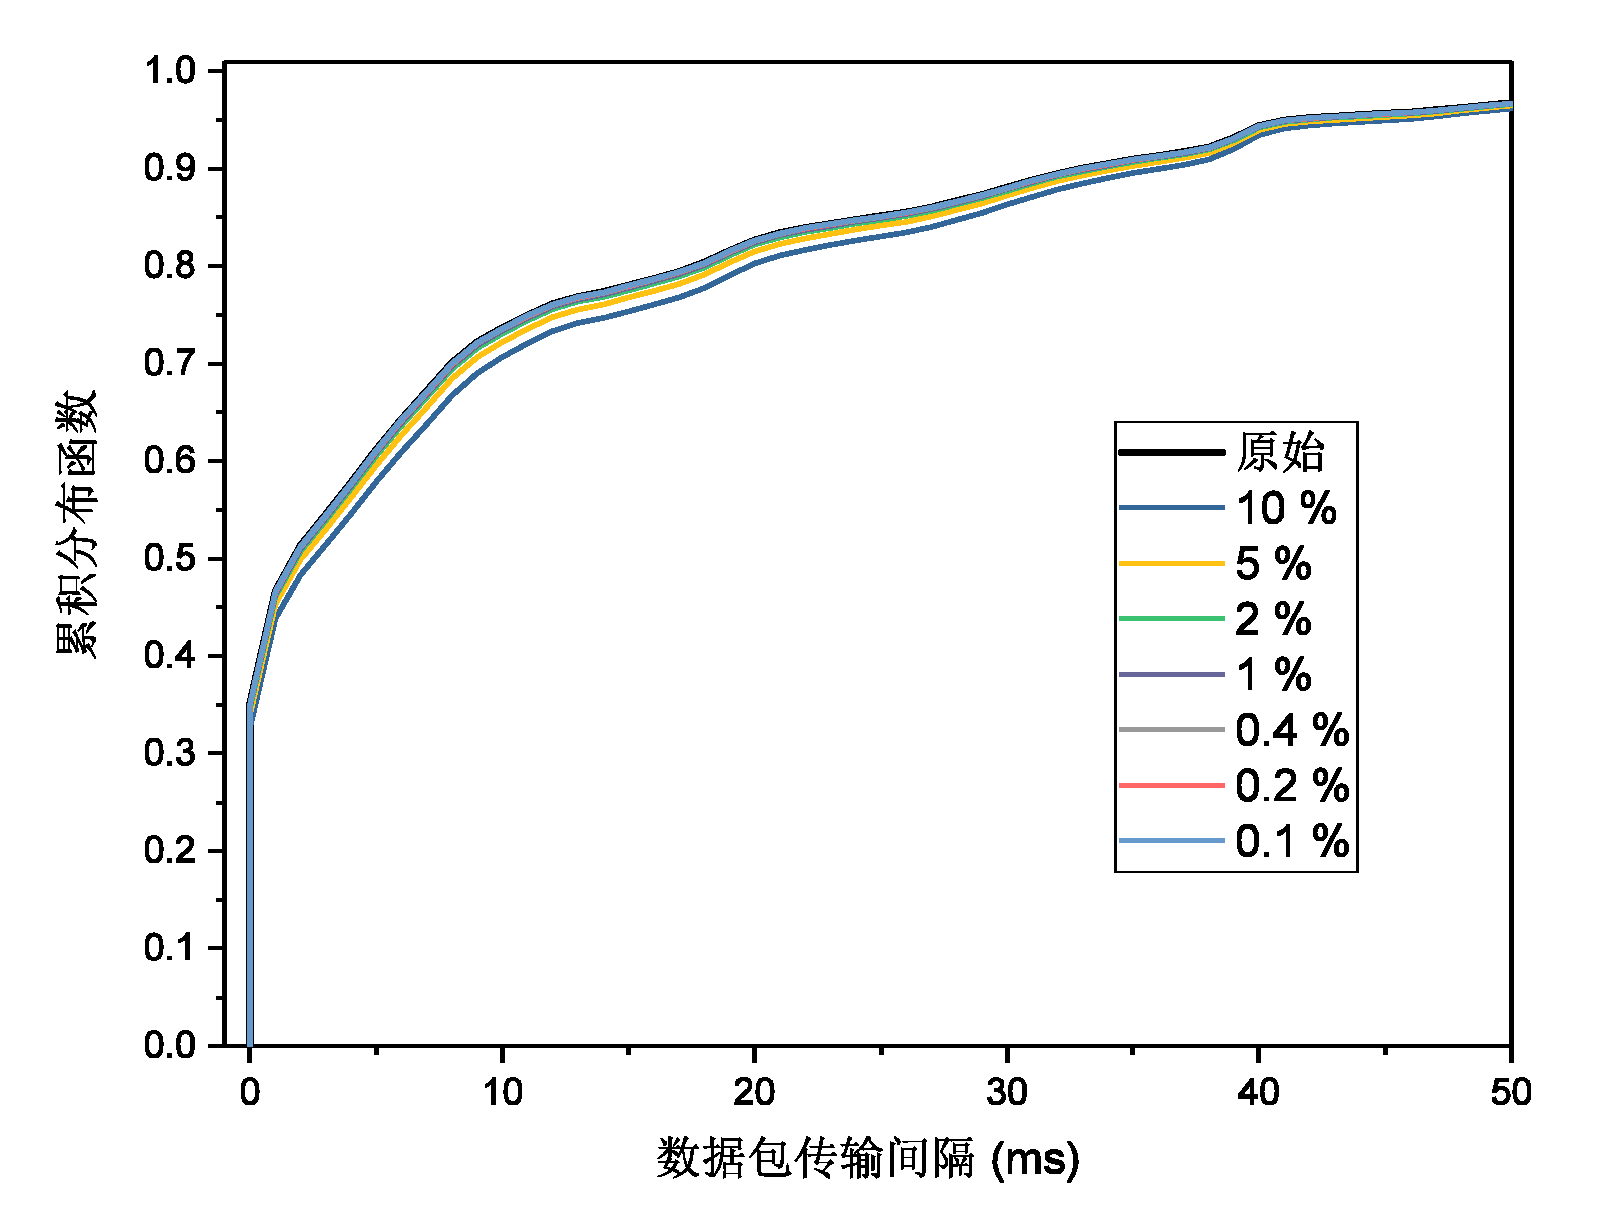
\includegraphics[width=0.48\textwidth]{chapters/chapter3/figures/ipd-cdf-excellent.pdf}
        }
        \subfigure[Good场景的CDF曲线]{
            \label{fig:3:result:ipd:cdf:good}
            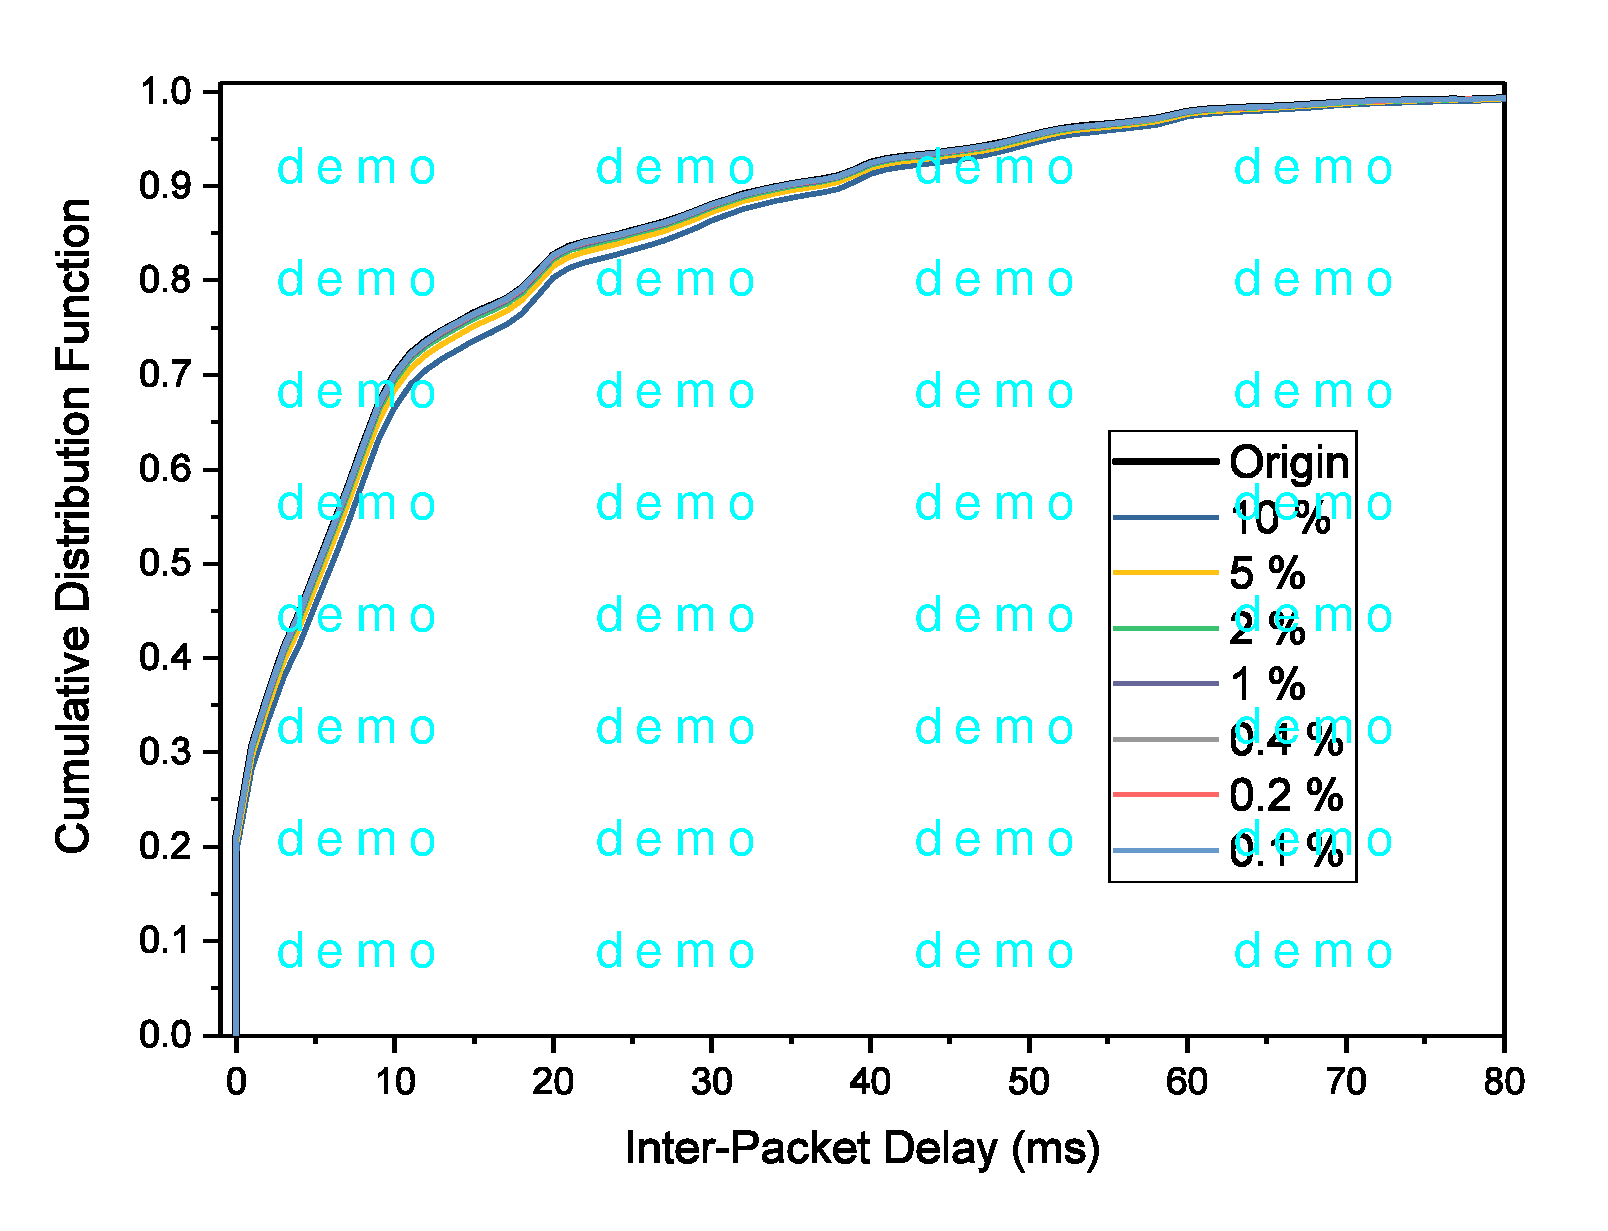
\includegraphics[width=0.48\textwidth]{chapters/chapter3/figures/ipd-cdf-good.pdf}
        }
        \caption{IPD分布的CDF曲线}
        \label{fig:3:result:ipd:cdf}
	\end{figure}
}

如图\ \nref{fig:3:result:ipd:cdf},虽然时间隐通道的分布与参照分布不完全重合,但总体趋势仍保持一致。即使主动丢包率上升到10\ \%,曲线仍未出现偏离。因此,时间隐通道的IPD分布可以通过CDF检测。

\subsubsection{条件熵检测结果}
\label{chap:analyze:result:ipd:kld}

\insertFigure{
    \begin{figure}[htb]
        \centering
        \subfigure[Excellent场景的箱线图]{
            \label{fig:3:result:ipd:kld:excellent}
            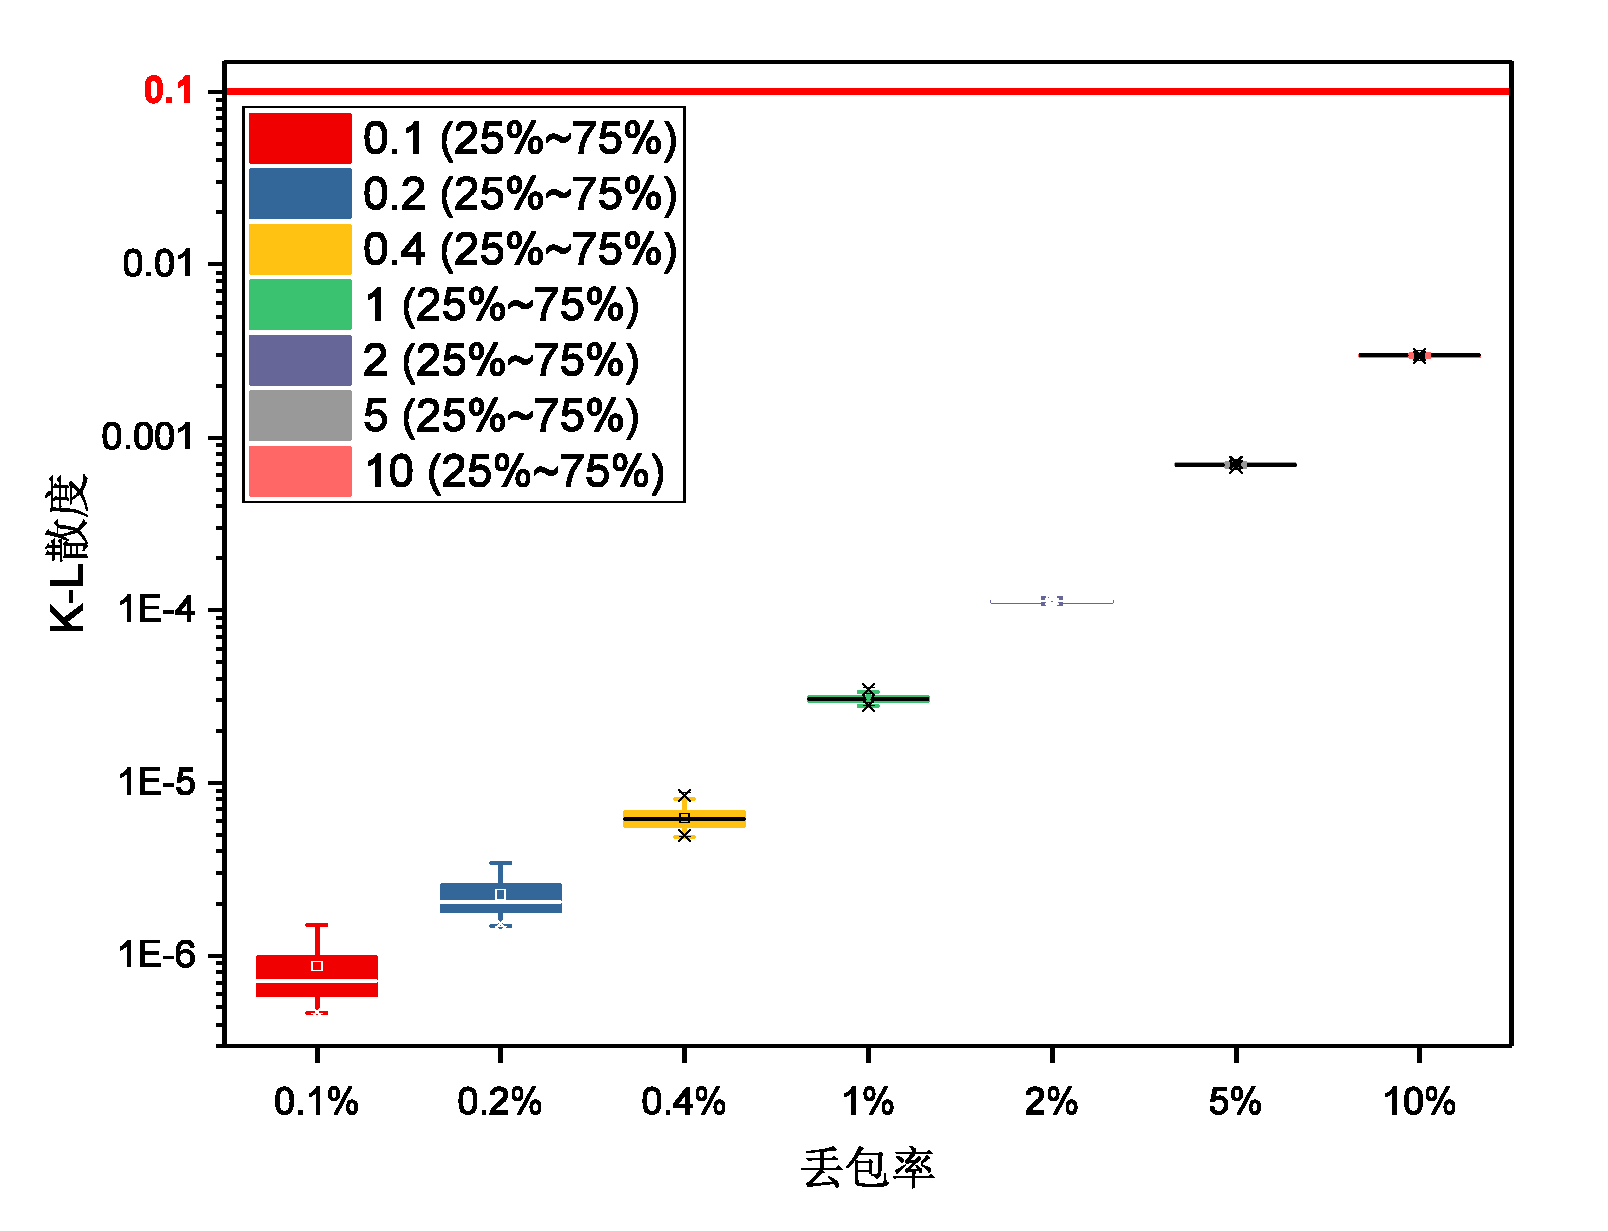
\includegraphics[width=0.48\textwidth]{chapters/chapter3/figures/ipd-kld-excellent.pdf}
        }
        \subfigure[Good场景的箱线图]{
            \label{fig:3:result:ipd:kld:good}
            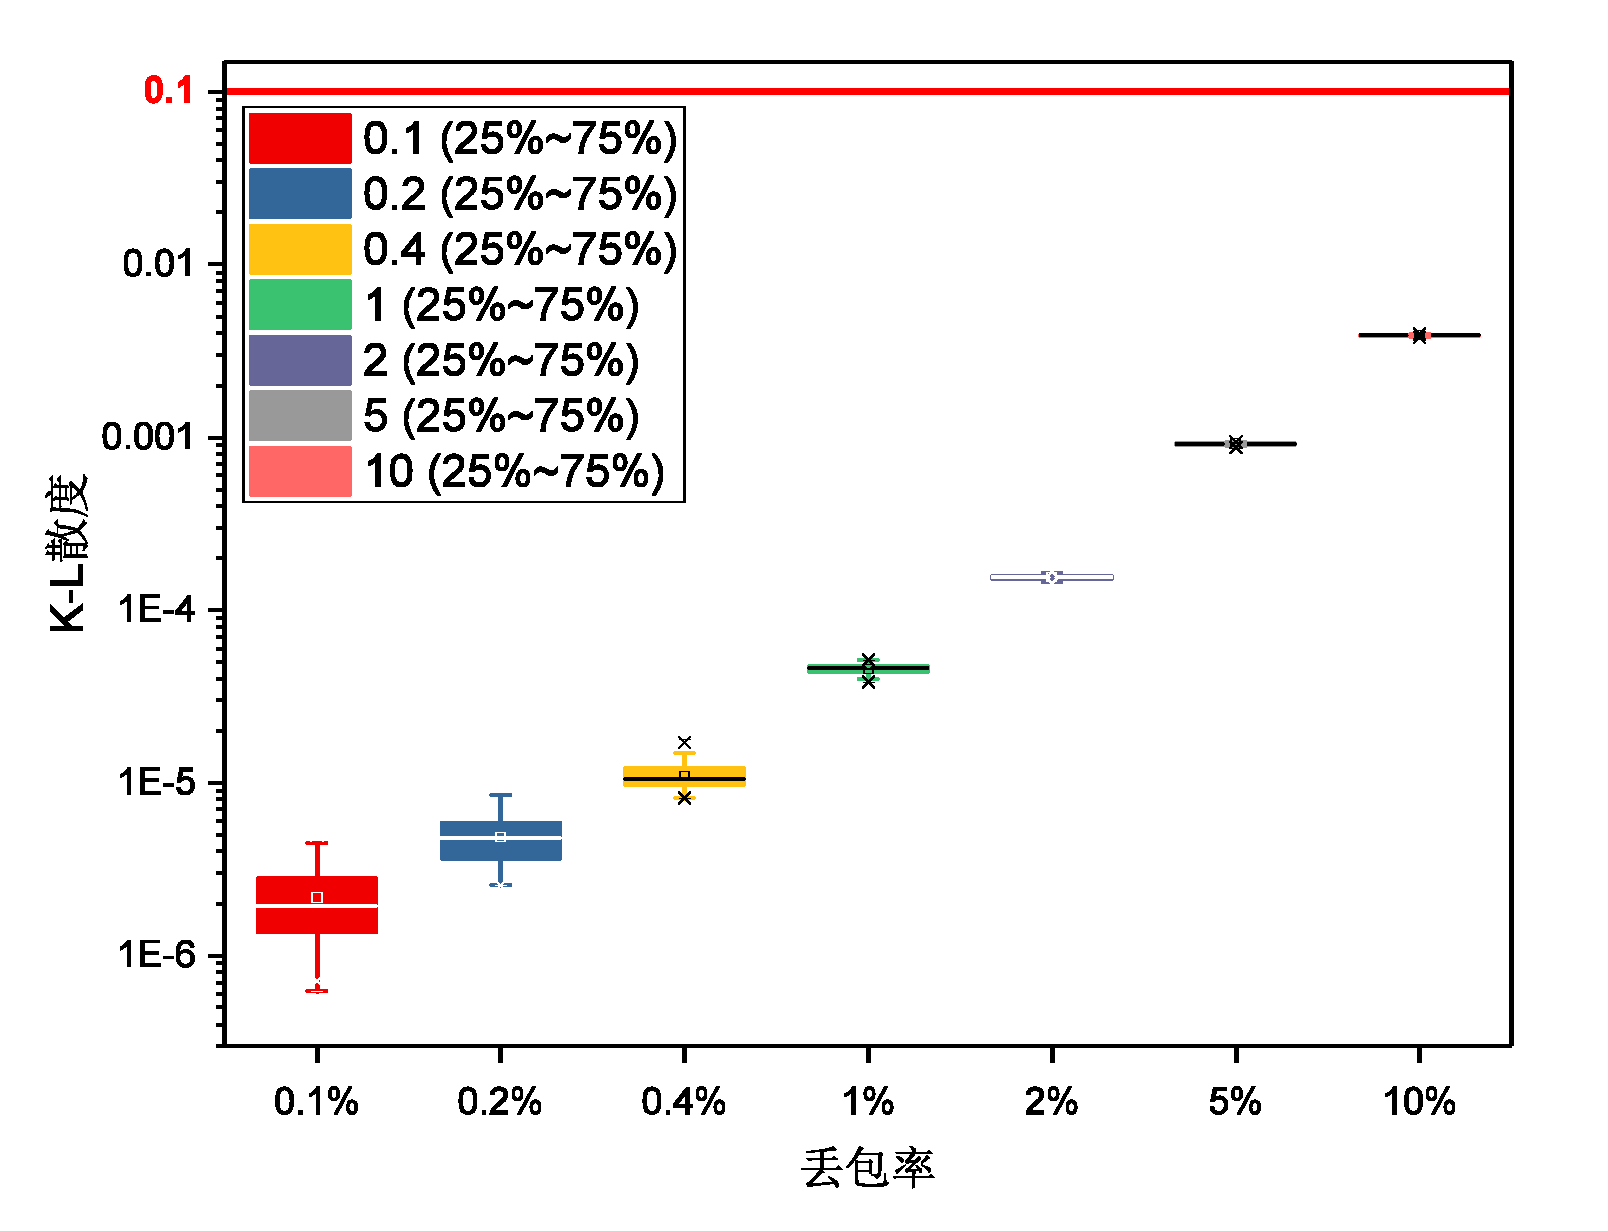
\includegraphics[width=0.48\textwidth]{chapters/chapter3/figures/ipd-kld-good.pdf}
        }
        \caption{IPD分布K-L散度检测结果的箱线图}
        \label{fig:3:result:ipd:kld}
	\end{figure}
}

如图\ \nref{fig:3:result:ipd:kld},两种场景中对IPD分布的条件熵检测结果汇总为箱线图。两种场景中,K-L散度检测结果均小于阈值0.1。随着主动丢包率的降低,K-L散度逐渐下降,意味着隐通道的IPD分布与宿主信道的IPD分布更加接近。

\subsubsection{一致性检验检测结果}
\label{chap:analyze:result:ipd:statistical}

\insertFigure{
    \begin{figure}[htb]
        \centering
        \subfigure[Excellent场景p值的箱线图]{
            \label{fig:3:result:ipd:ks:excellent}
            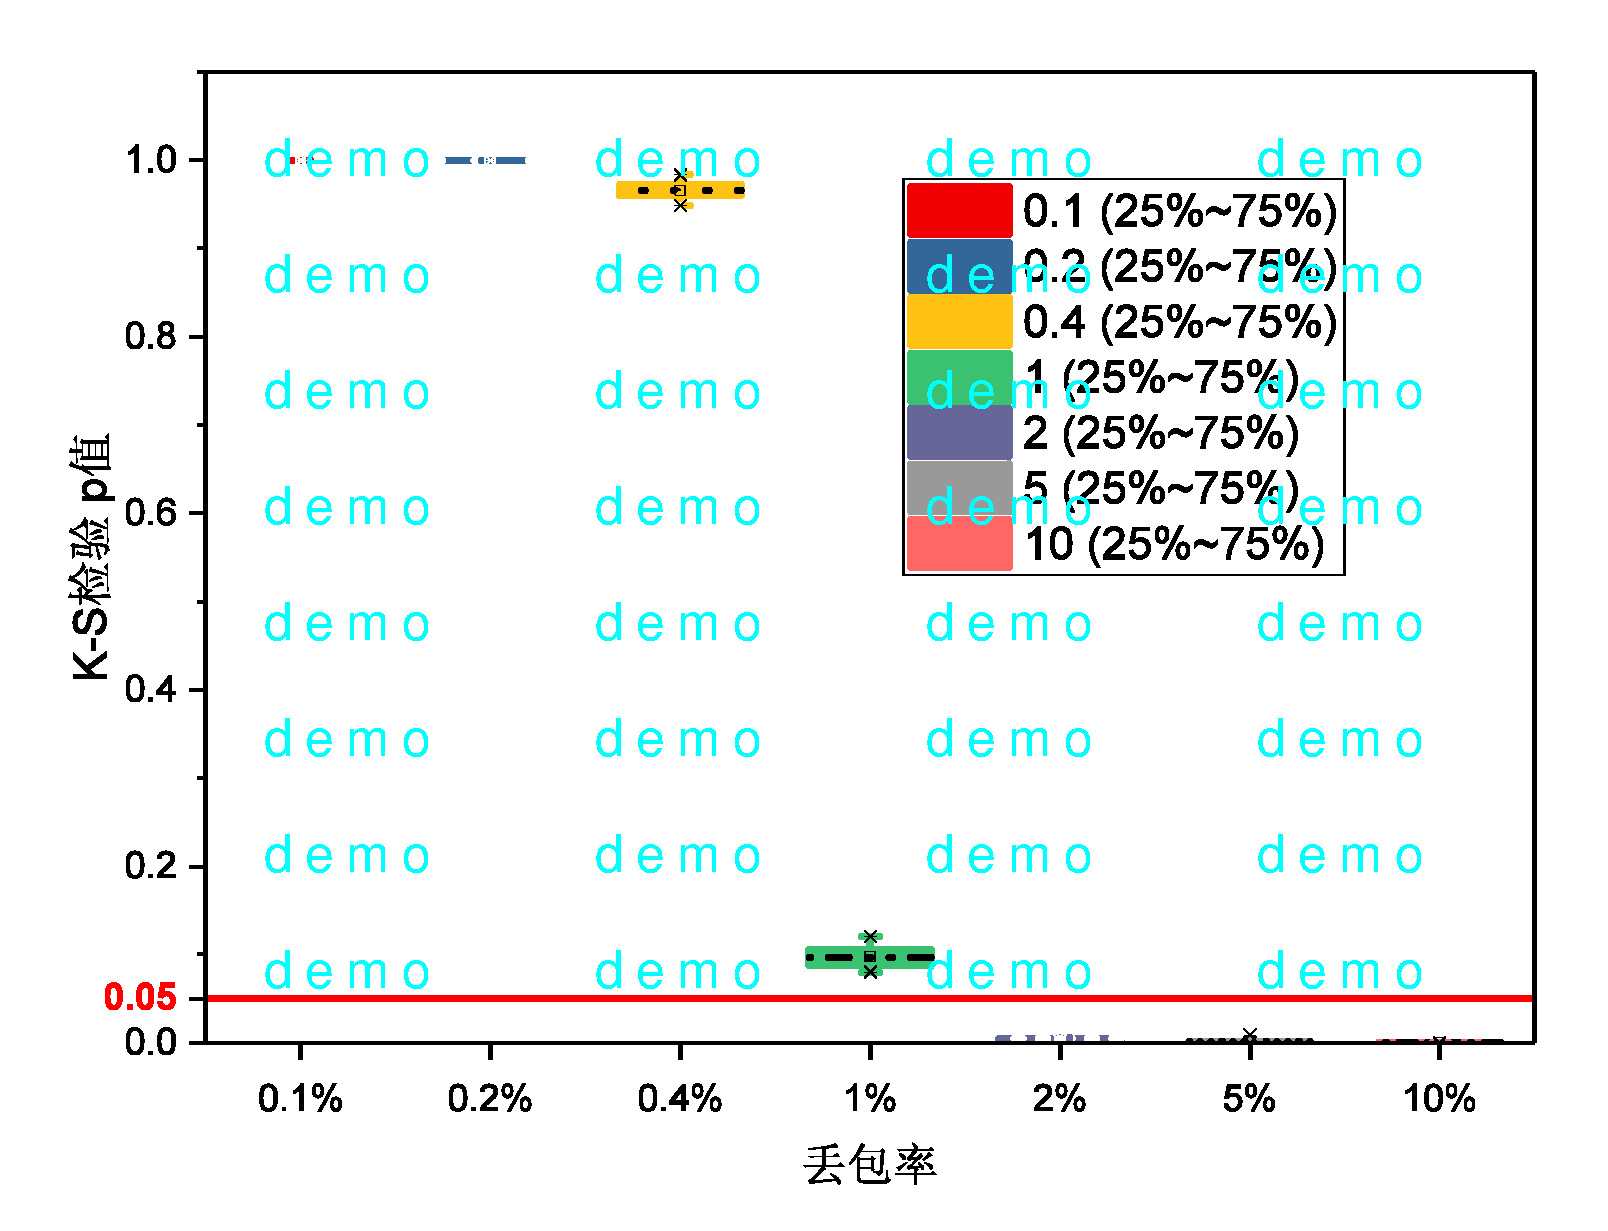
\includegraphics[width=0.48\textwidth]{chapters/chapter3/figures/ipd-ks-excellent.pdf}
        }
        \subfigure[Good场景p值的箱线图]{
            \label{fig:3:result:ipd:ks:good}
            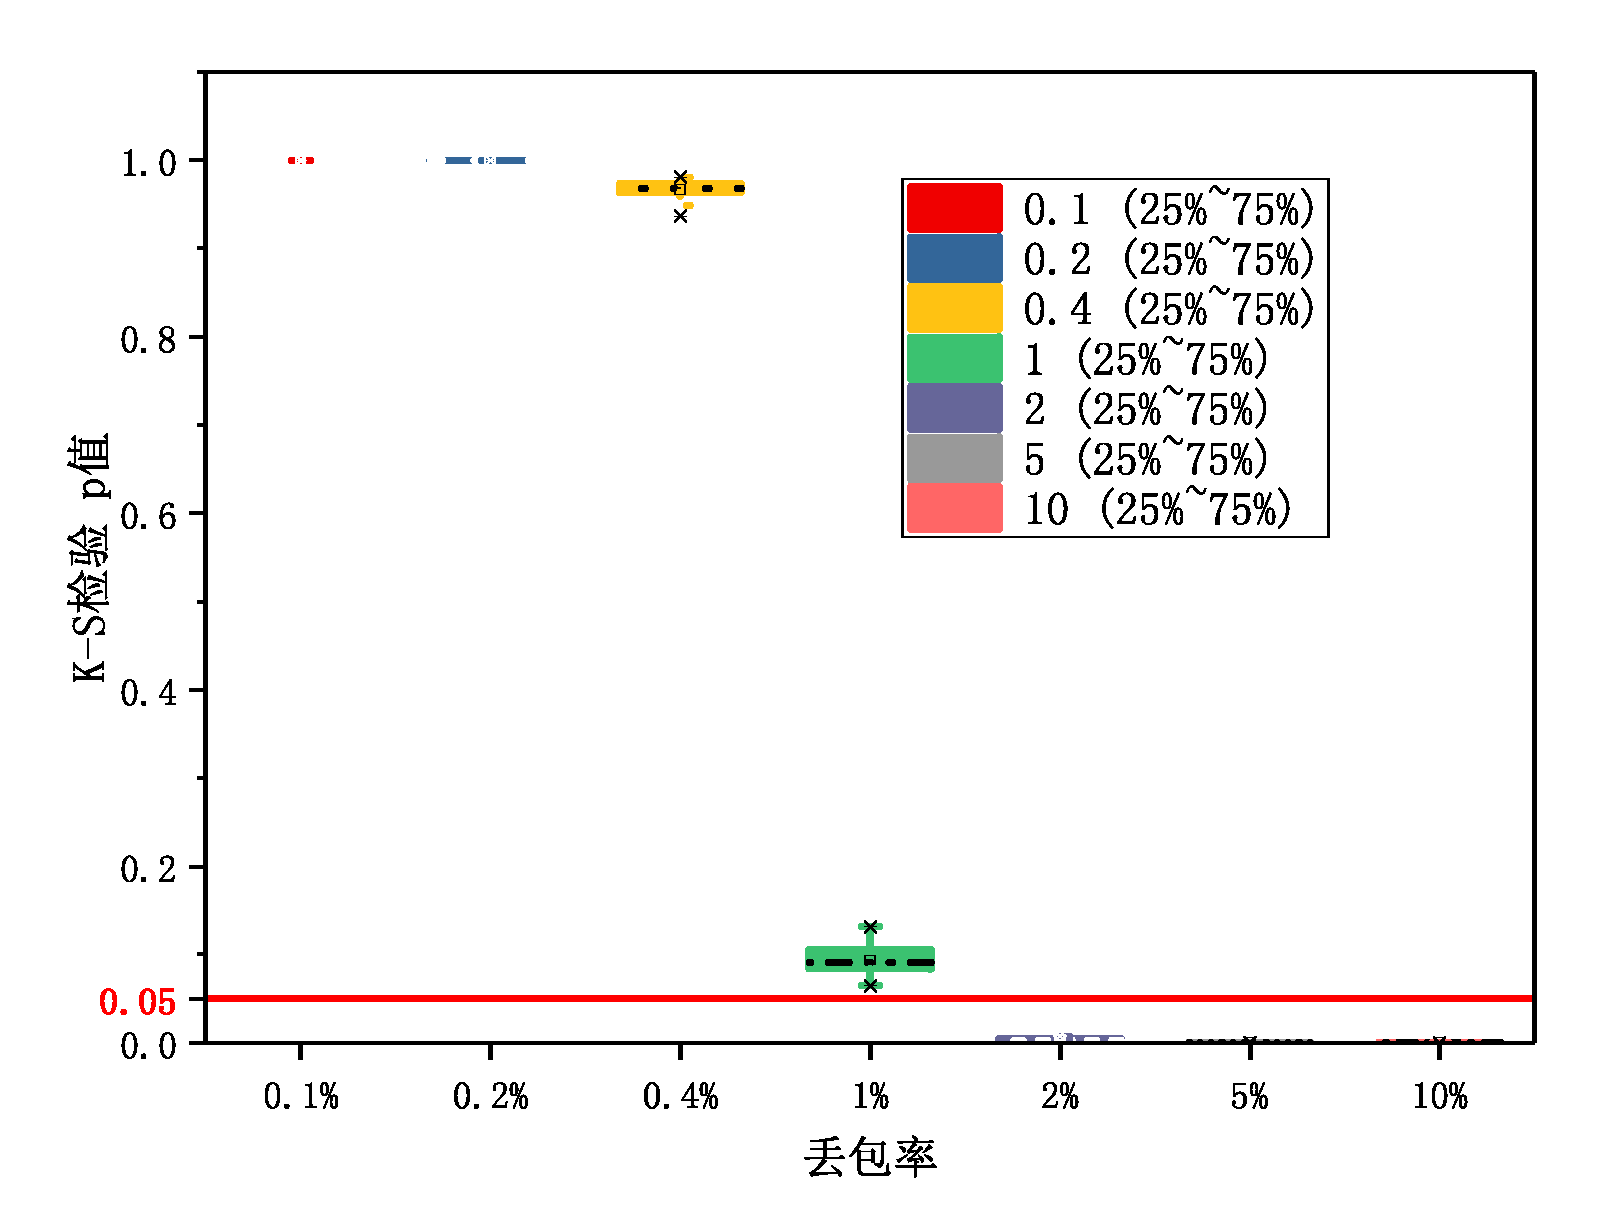
\includegraphics[width=0.48\textwidth]{chapters/chapter3/figures/ipd-ks-good.pdf}
        }
        \caption{IPD分布K-S检验结果的箱线图}
        \label{fig:3:result:ipd:ks}
	\end{figure}

	\begin{figure}[htb]
        \centering
        \subfigure[Excellent场景p值的箱线图]{
            \label{fig:3:result:ipd:t:excellent}
            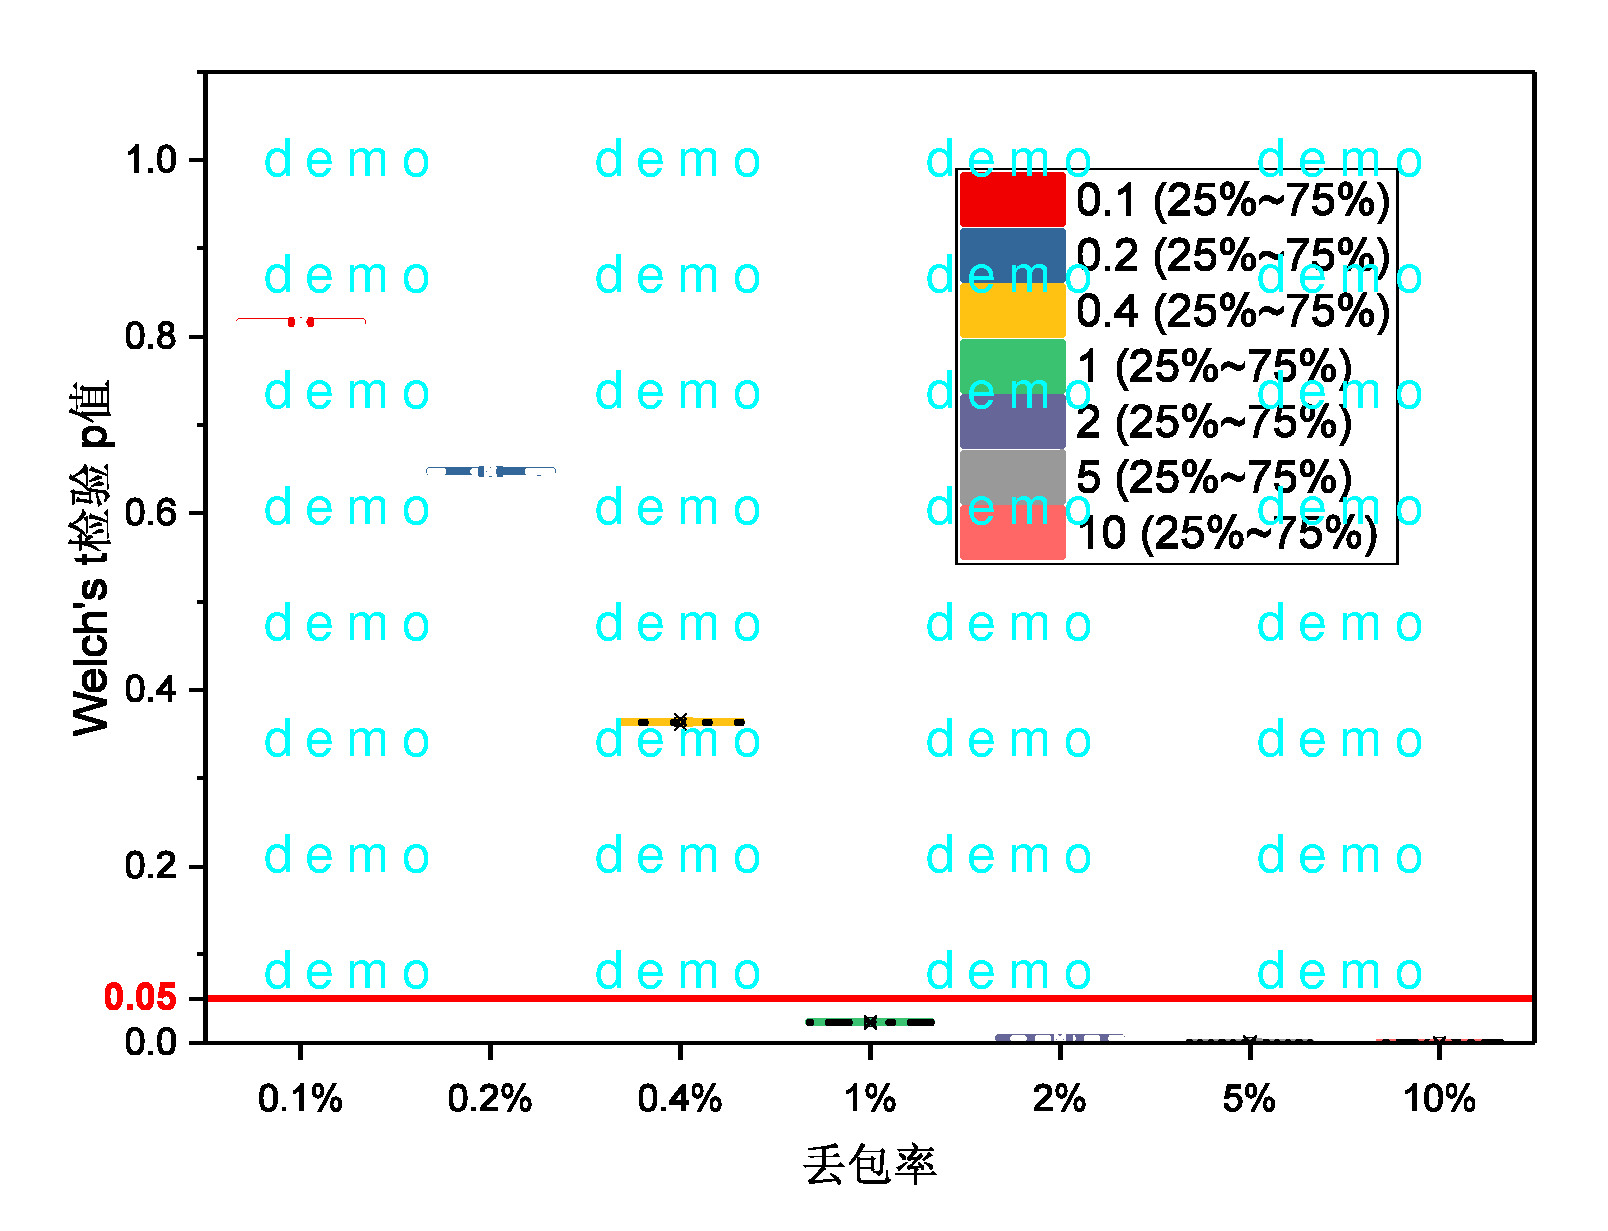
\includegraphics[width=0.48\textwidth]{chapters/chapter3/figures/ipd-t-excellent.pdf}
        }
        \subfigure[Good场景p值的箱线图]{
            \label{fig:3:result:ipd:t:good}
            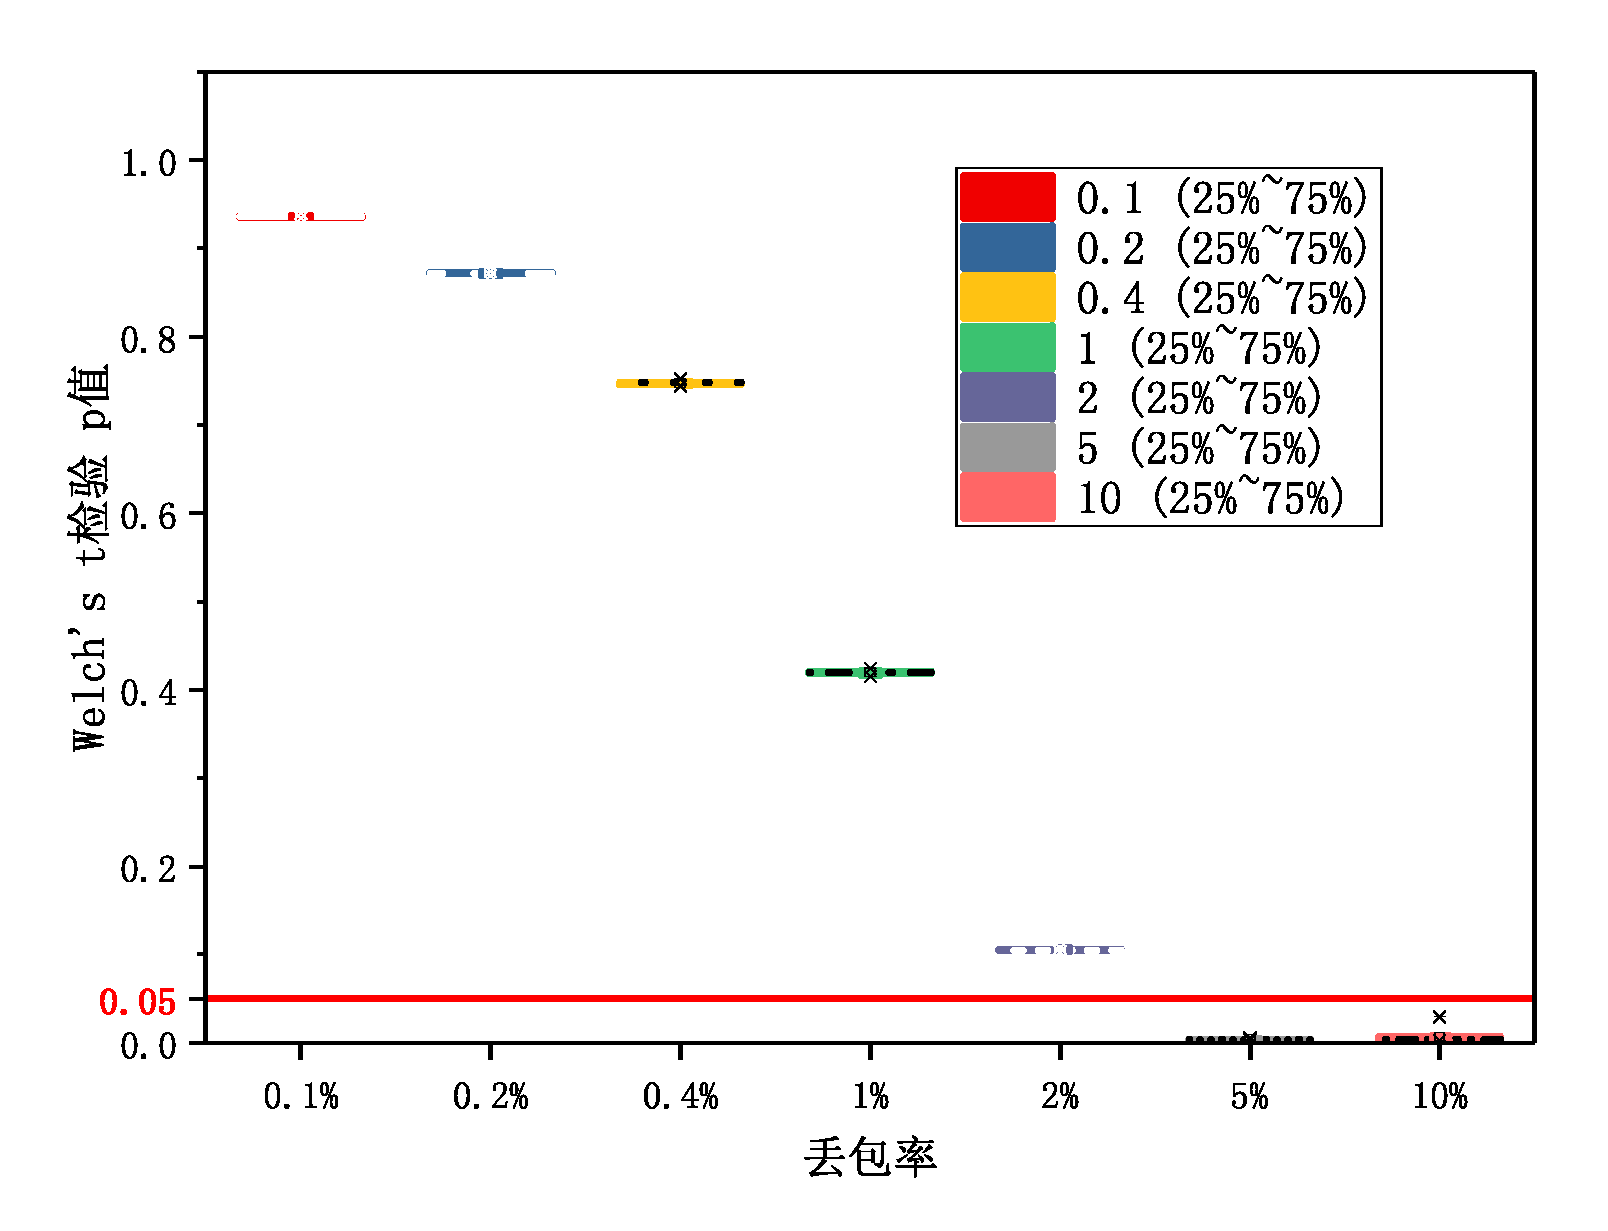
\includegraphics[width=0.48\textwidth]{chapters/chapter3/figures/ipd-t-good.pdf}
        }
        \caption{IPD分布Welch's t检验结果的箱线图}
        \label{fig:3:result:ipd:t}
	\end{figure}

	\begin{figure}[htb]
        \centering
        \subfigure[Excellent场景p值的箱线图]{
            \label{fig:3:result:ipd:mw:excellent}
            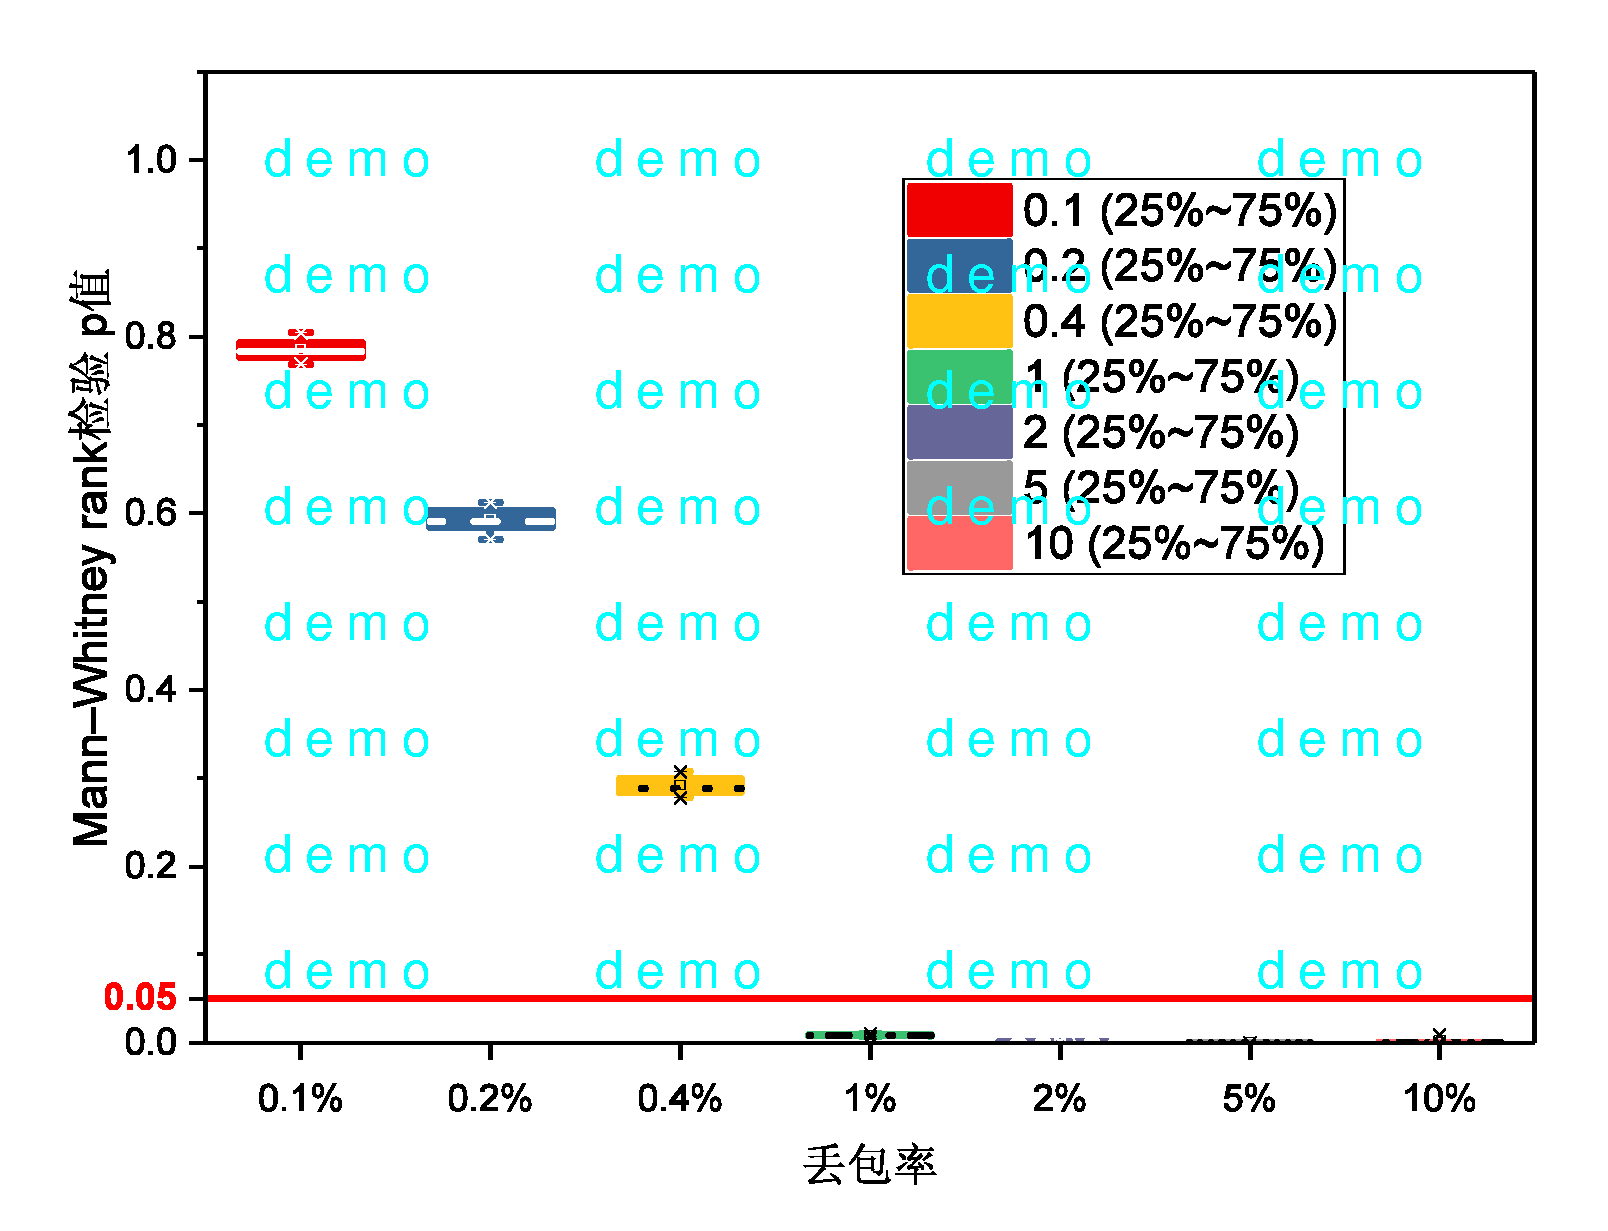
\includegraphics[width=0.48\textwidth]{chapters/chapter3/figures/ipd-mw-excellent.pdf}
        }
        \subfigure[Good场景p值的箱线图]{
            \label{fig:3:result:ipd:mw:good}
            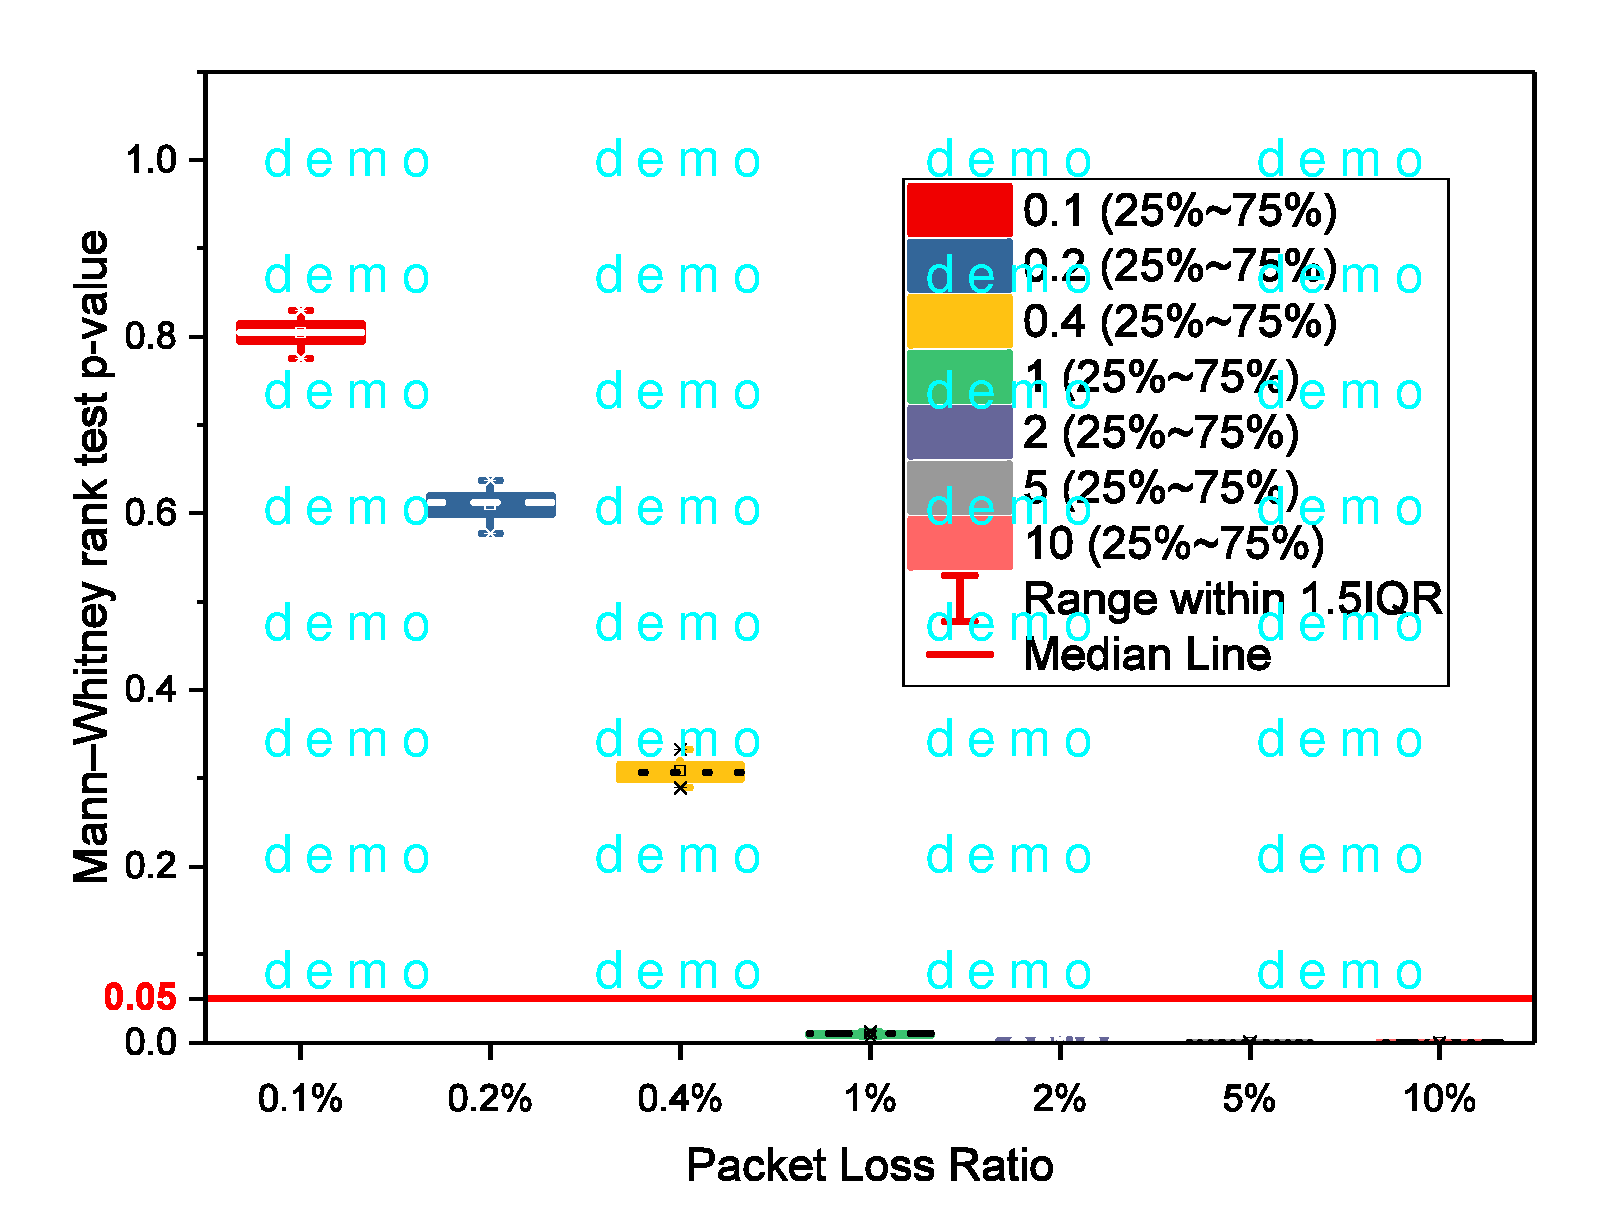
\includegraphics[width=0.48\textwidth]{chapters/chapter3/figures/ipd-mw-good.pdf}
        }
        \caption{IPD分布Mann–Whitney rank检验结果的箱线图}
        \label{fig:3:result:ipd:mw}
	\end{figure}
}

如图\ \nref{fig:3:result:ipd:ks},通过K-S检验,已经检测出部分时间隐通道。当主动丢包率$\le 1\ \%$时,IPD分布通过了K-S检验,并且随着主动丢包率的进一步降低,K-S检验的p值逐渐增大。如图\ \nref{fig:3:result:ipd:t},Welch's t检验中,已经检测出大部分时间隐通道。Excellent场景中,当主动丢包率$\le 0.4\ \%$后,才通过Welch's t检验;而Good场景中,当主动丢包率$\le 2\ \%$时,即可通过Welch's t检验。Welch's t检验结果表明,不同的场景中,丢包导致的IPD平均值变化程度不同。

如图\ \nref{fig:3:result:ipd:mw},Mann–Whitney rank检验中,只有主动丢包率$\le 0.4\ \%$才通过检测。由于Mann–Whitney rank检验适用的样本分布为均匀分布,所以检验结果较Welch's t检验更加严格。

\subsubsection{相对距离检测结果}
\label{chap:analyze:result:ipd:distance}

\insertFigure{
	\begin{figure}[htb]
        \centering
        \subfigure[Excellent场景Wasserstein距离的箱线图]{
            \label{fig:3:result:ipd:wd:excellent}
            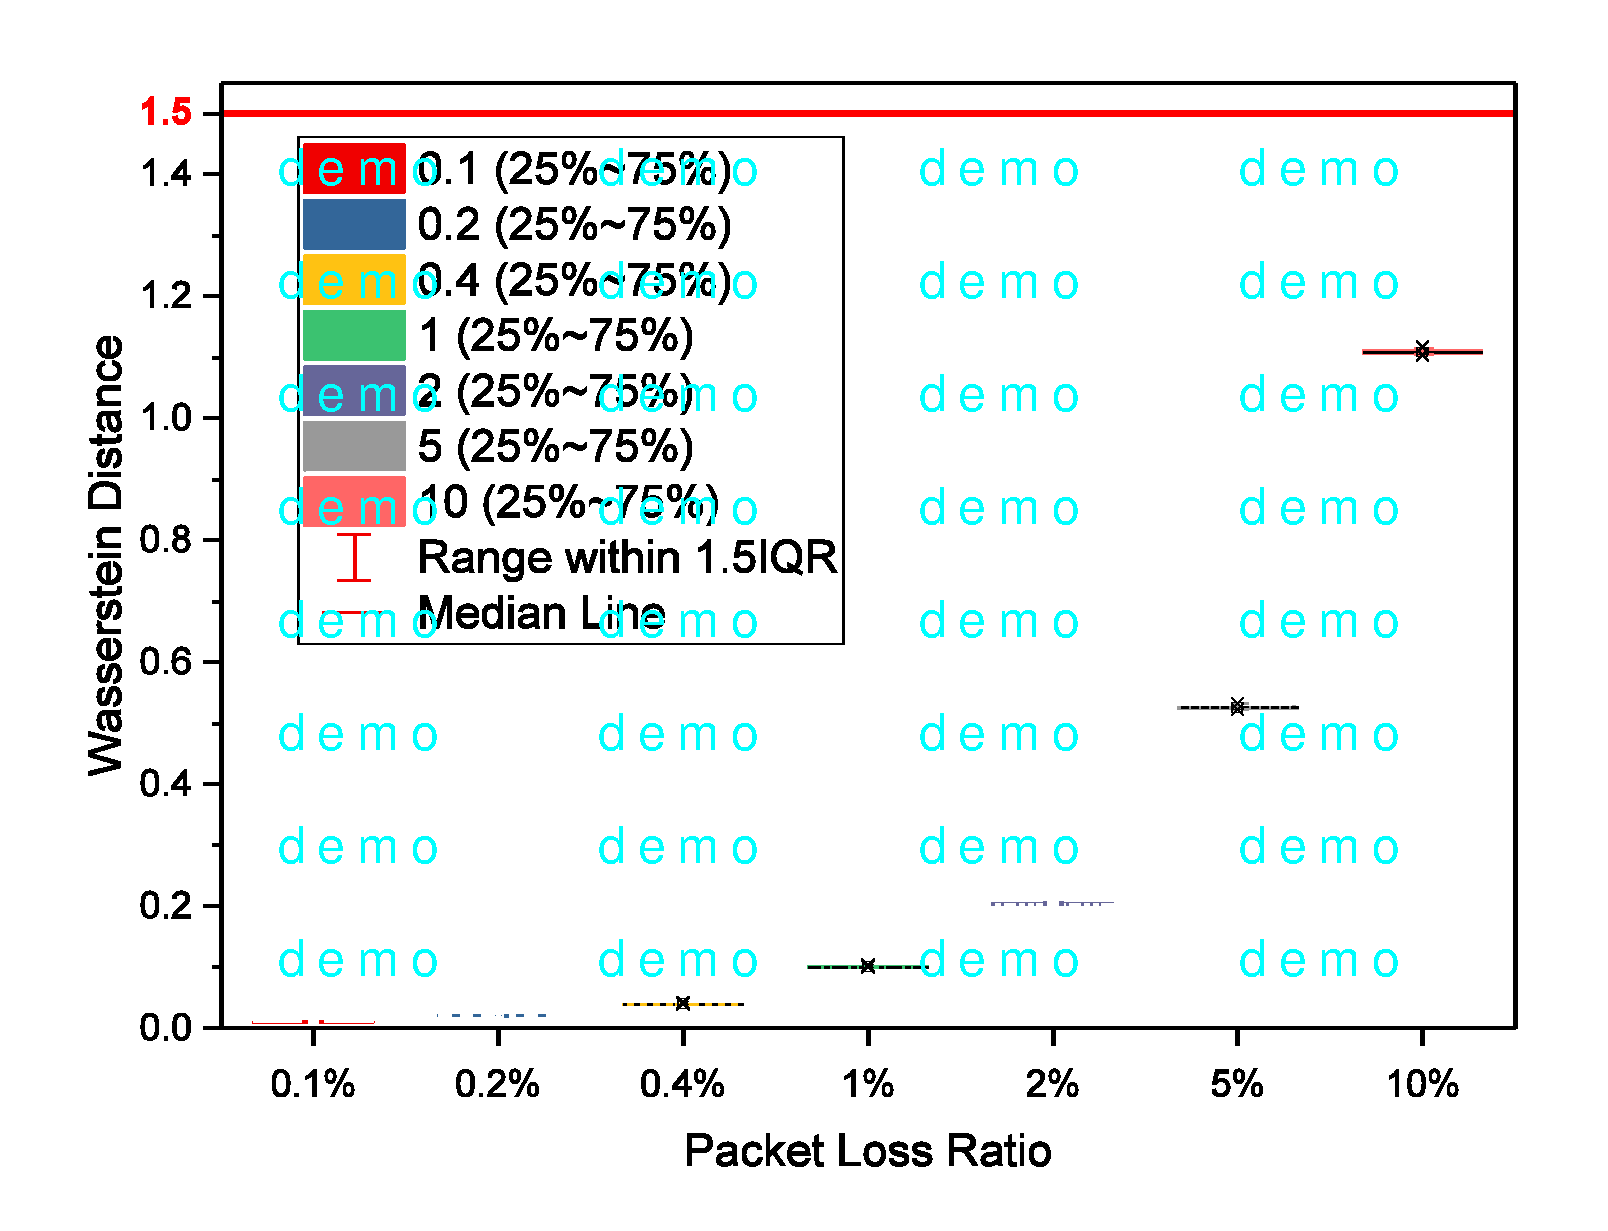
\includegraphics[width=0.48\textwidth]{chapters/chapter3/figures/ipd-wd-excellent.pdf}
        }
        \subfigure[Good场景Wasserstein距离的箱线图]{
            \label{fig:3:result:ipd:wd:good}
            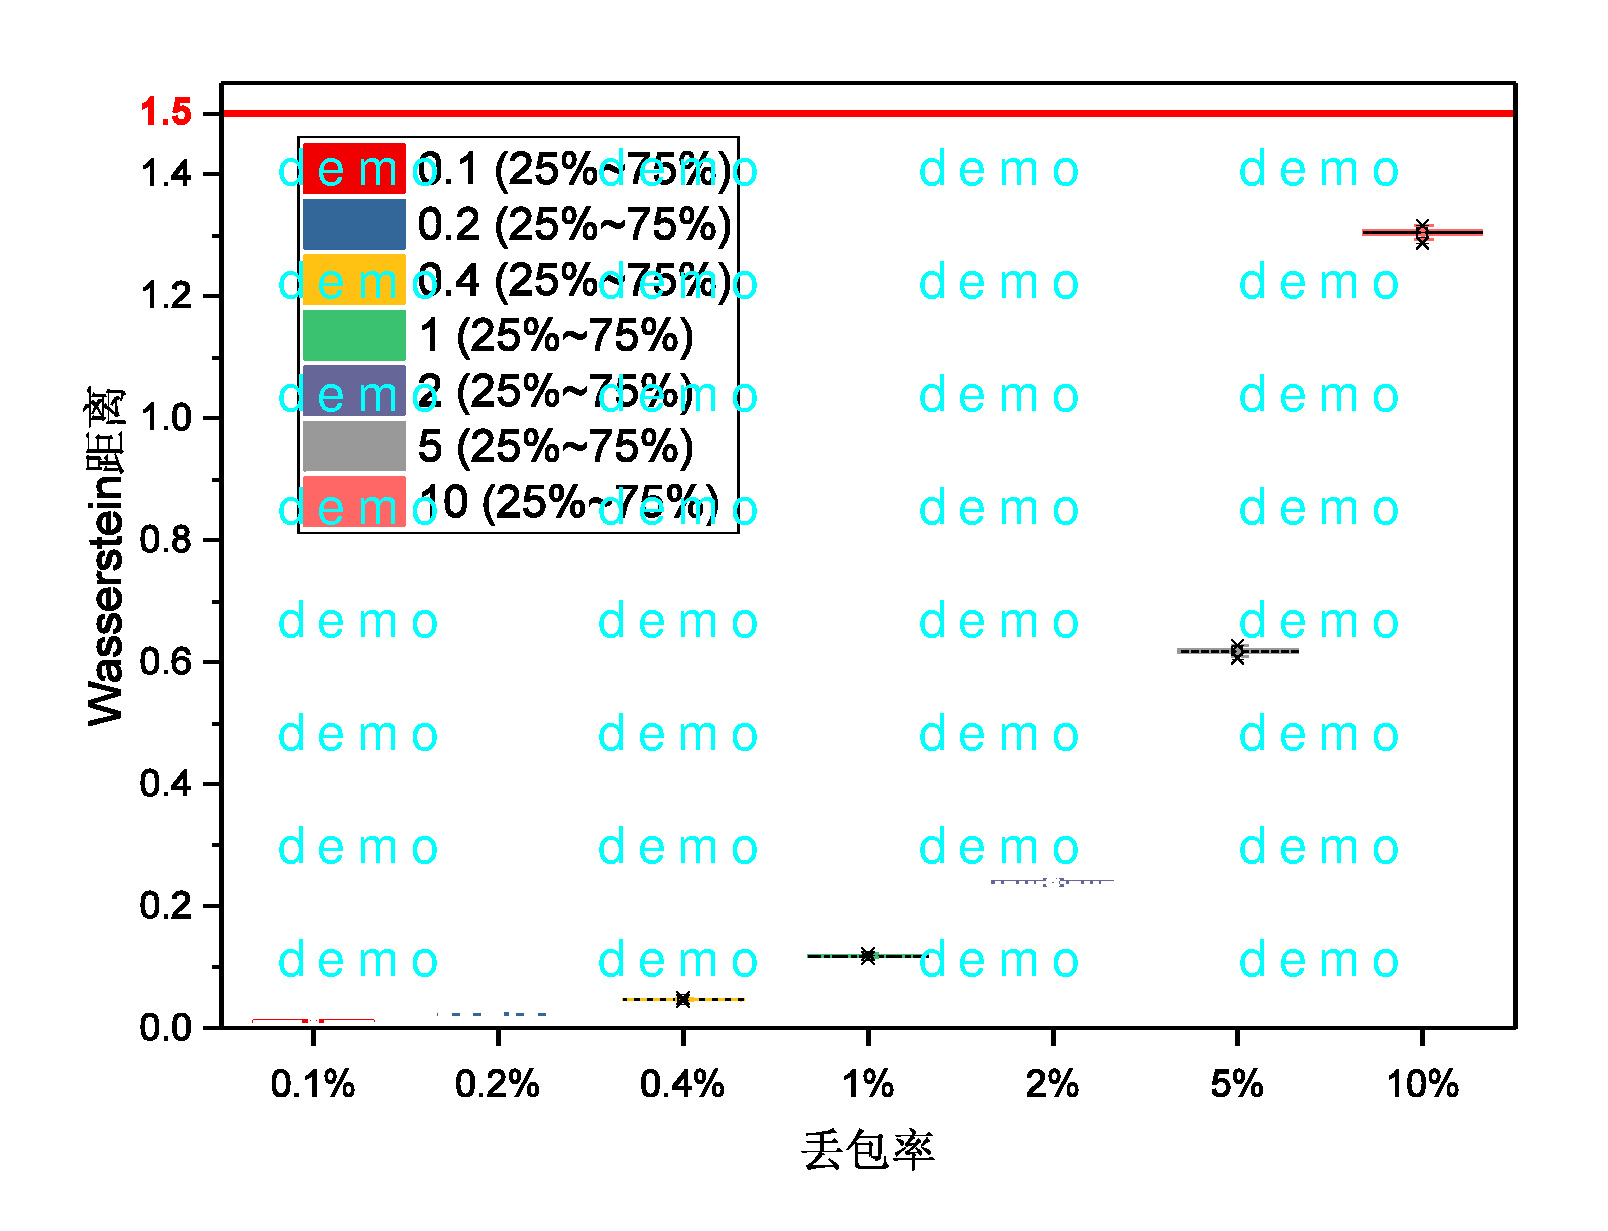
\includegraphics[width=0.48\textwidth]{chapters/chapter3/figures/ipd-wd-good.pdf}
        }
        \caption{IPD分布Wasserstein距离检测的箱线图}
        \label{fig:3:result:ipd:wd}
	\end{figure}

	\begin{figure}[htb]
        \centering
        \subfigure[Excellent场景能量距离的箱线图]{
            \label{fig:3:result:ipd:ed:excellent}
            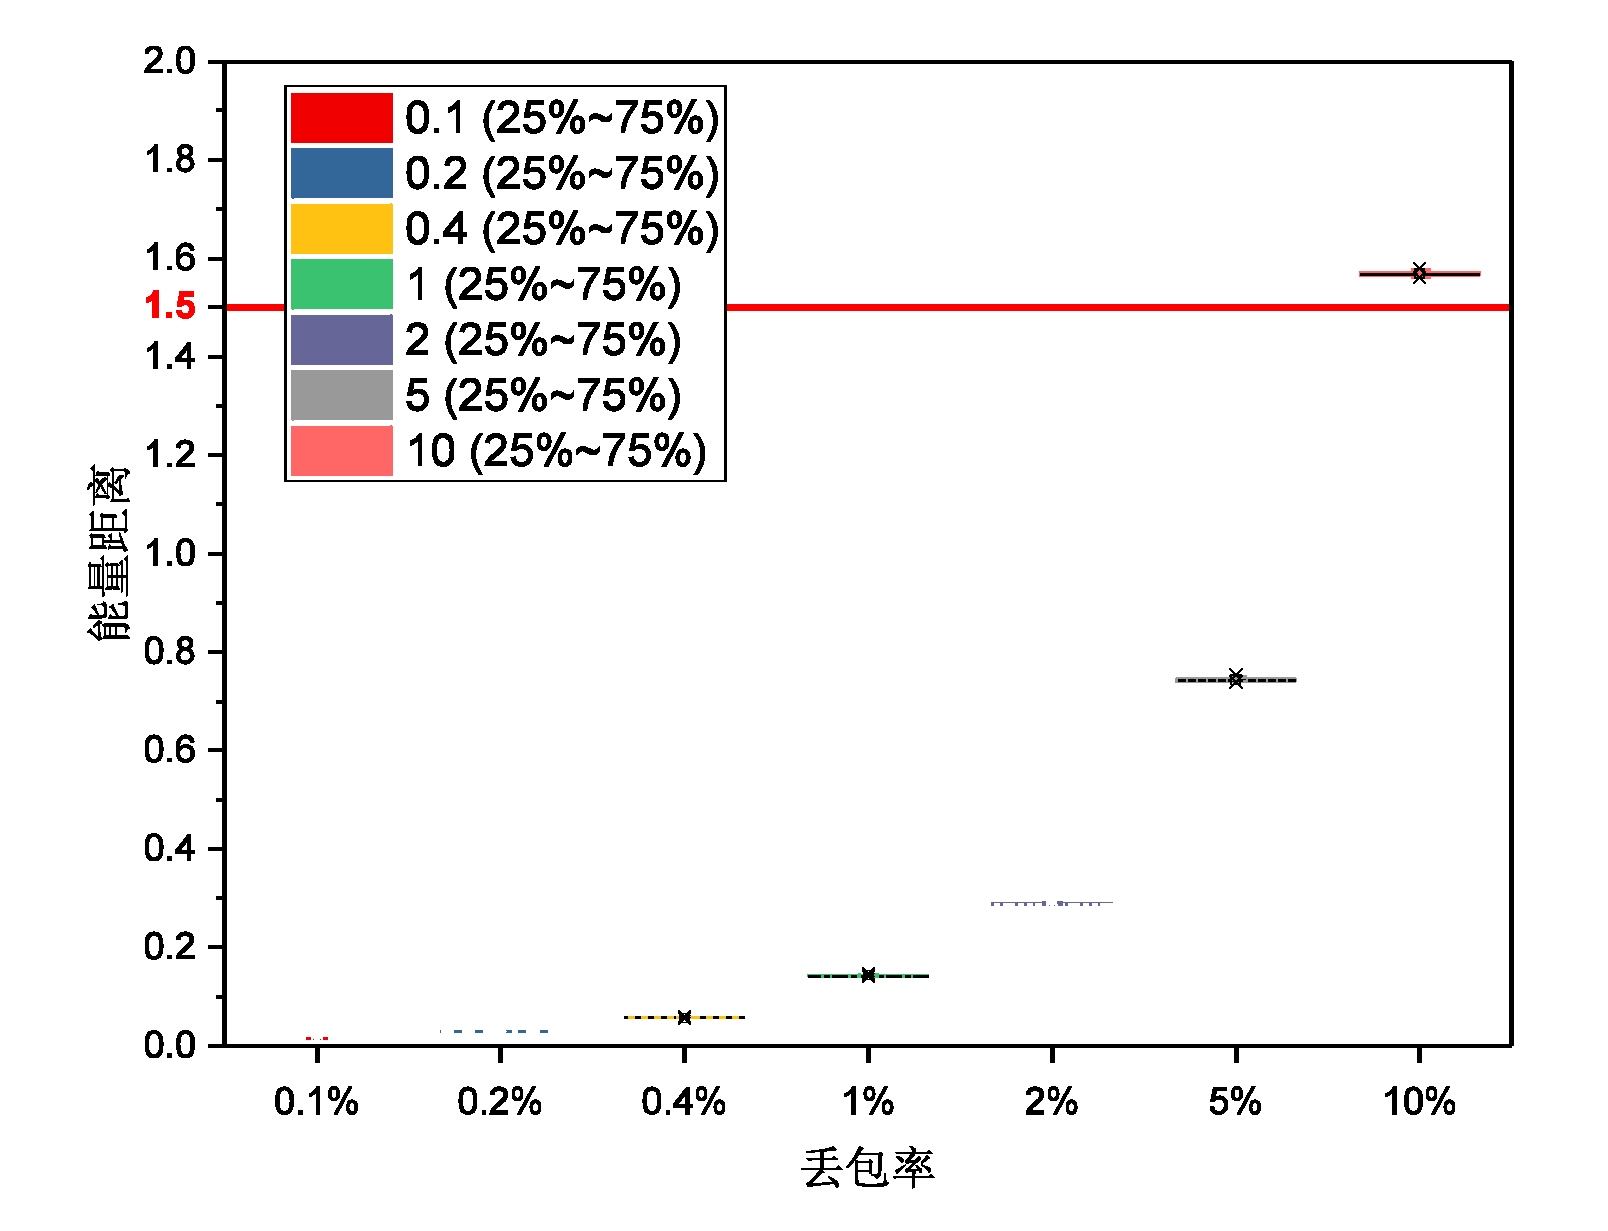
\includegraphics[width=0.48\textwidth]{chapters/chapter3/figures/ipd-ed-excellent.pdf}
        }
        \subfigure[Good场景能量距离的箱线图]{
            \label{fig:3:result:ipd:ed:good}
            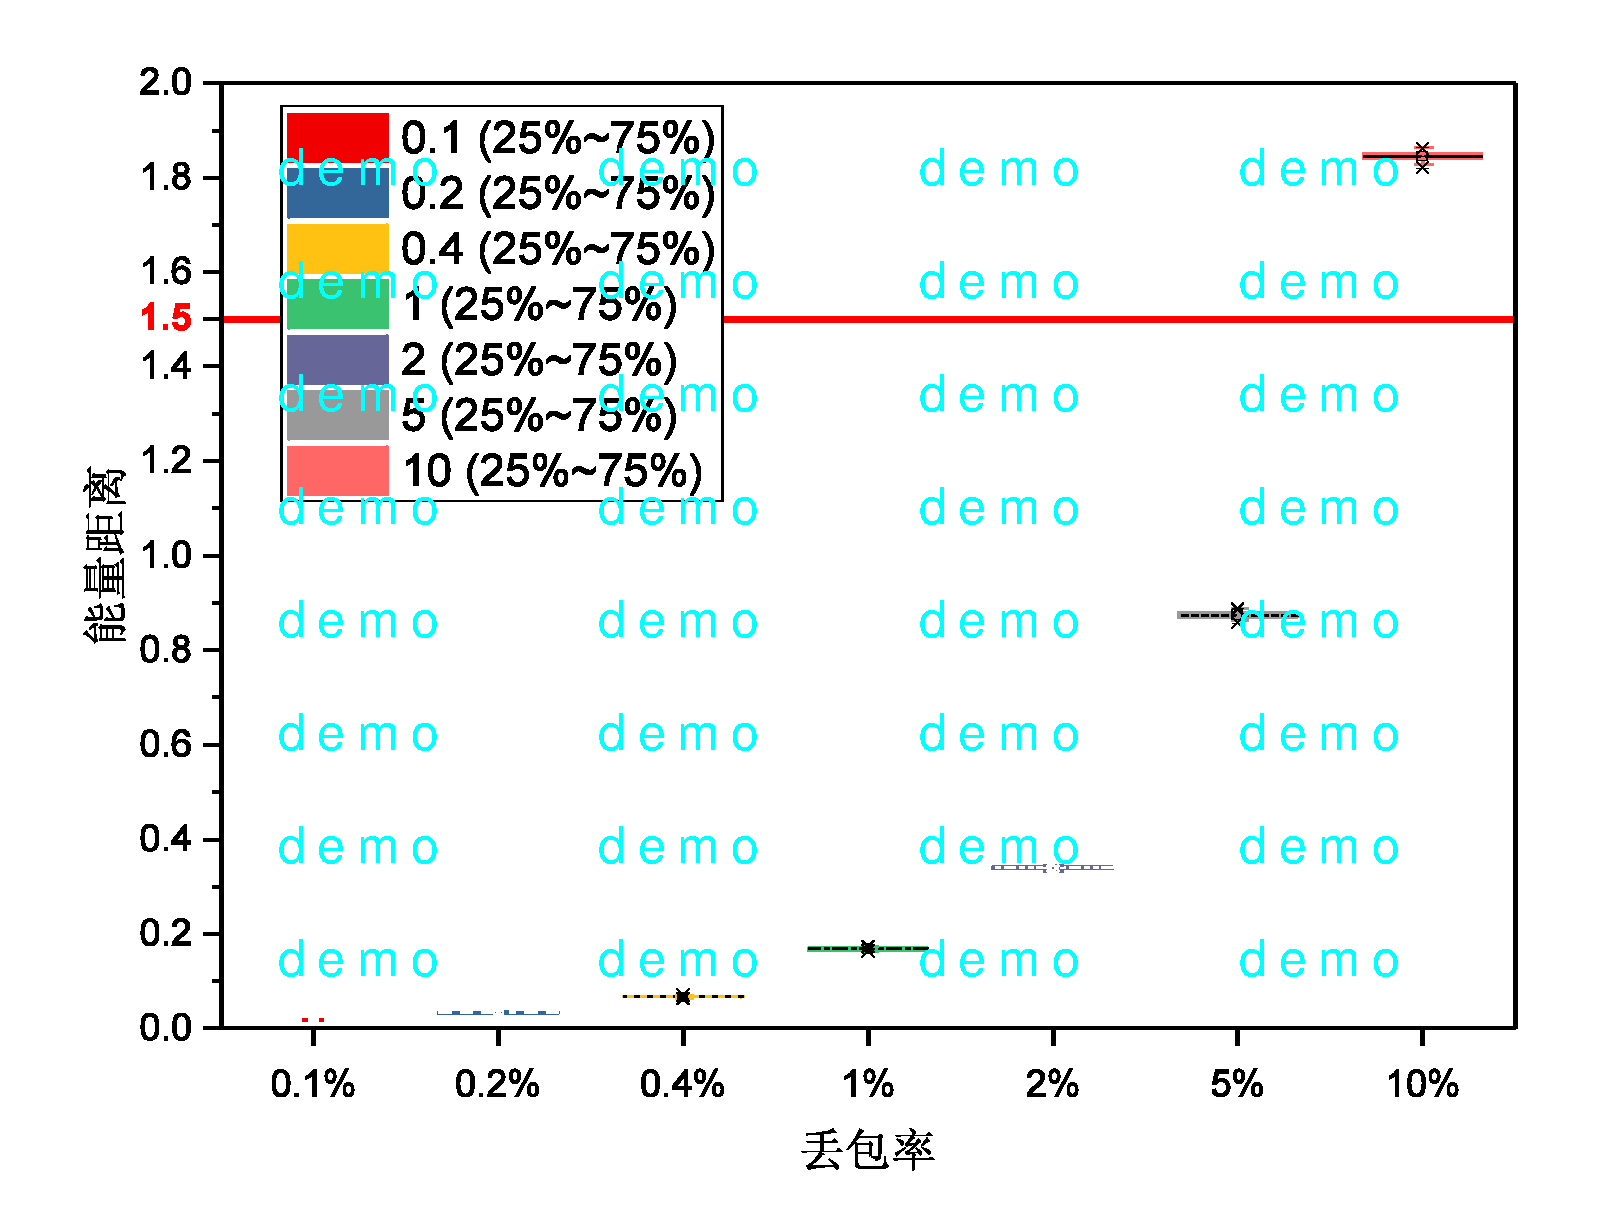
\includegraphics[width=0.48\textwidth]{chapters/chapter3/figures/ipd-ed-good.pdf}
        }
        \caption{IPD分布能量距离检测的箱线图}
        \label{fig:3:result:ipd:ed}
	\end{figure}
}

如图\ \nref{fig:3:result:ipd:wd},主动丢包率与Wasserstein距离呈正相关。两种场景中检测结果相同,虽然当主动丢包率为$10\ \%$时已经接近阈值,但仍未超过阈值,因此无法断定为时间隐通道。如图\ \nref{fig:3:result:ipd:ed},能量距离与主动丢包率也呈正相关。两种场景中,当主动丢包率$\le 5\ \%$时,才可通过检测。根据检测结果,能量距离较Wasserstein距离具有更高的要求,但二者具有一致的变化趋势。

根据以上测试结果,通过IPD分布检测基于主动丢包的时间隐通道,在灵敏度方面无法达到检测要求。其主要因素,在于丢包事件数量与IPD数量相比较少,少量的丢包不会导致IPD分布出现较大变动。因此,现有基于IPD的检测方法,无法有效检测基于主动丢包的时间隐通道。另一方面,实验结果表明,在当前的检测方法面前,基于主动丢包的时间隐通道具有较好的隐蔽性。

\subsection{连续丢包数检测结果评估}
\label{chap:analyze:result:burst}

\subsubsection{CDF检测结果}
\label{chap:analyze:result:burst:cdf}

\insertFigure{
    \begin{figure}[htb]
        \centering
        \subfigure[Excellent场景的CDF曲线]{
            \label{fig:3:result:burst:cdf:excellent}
            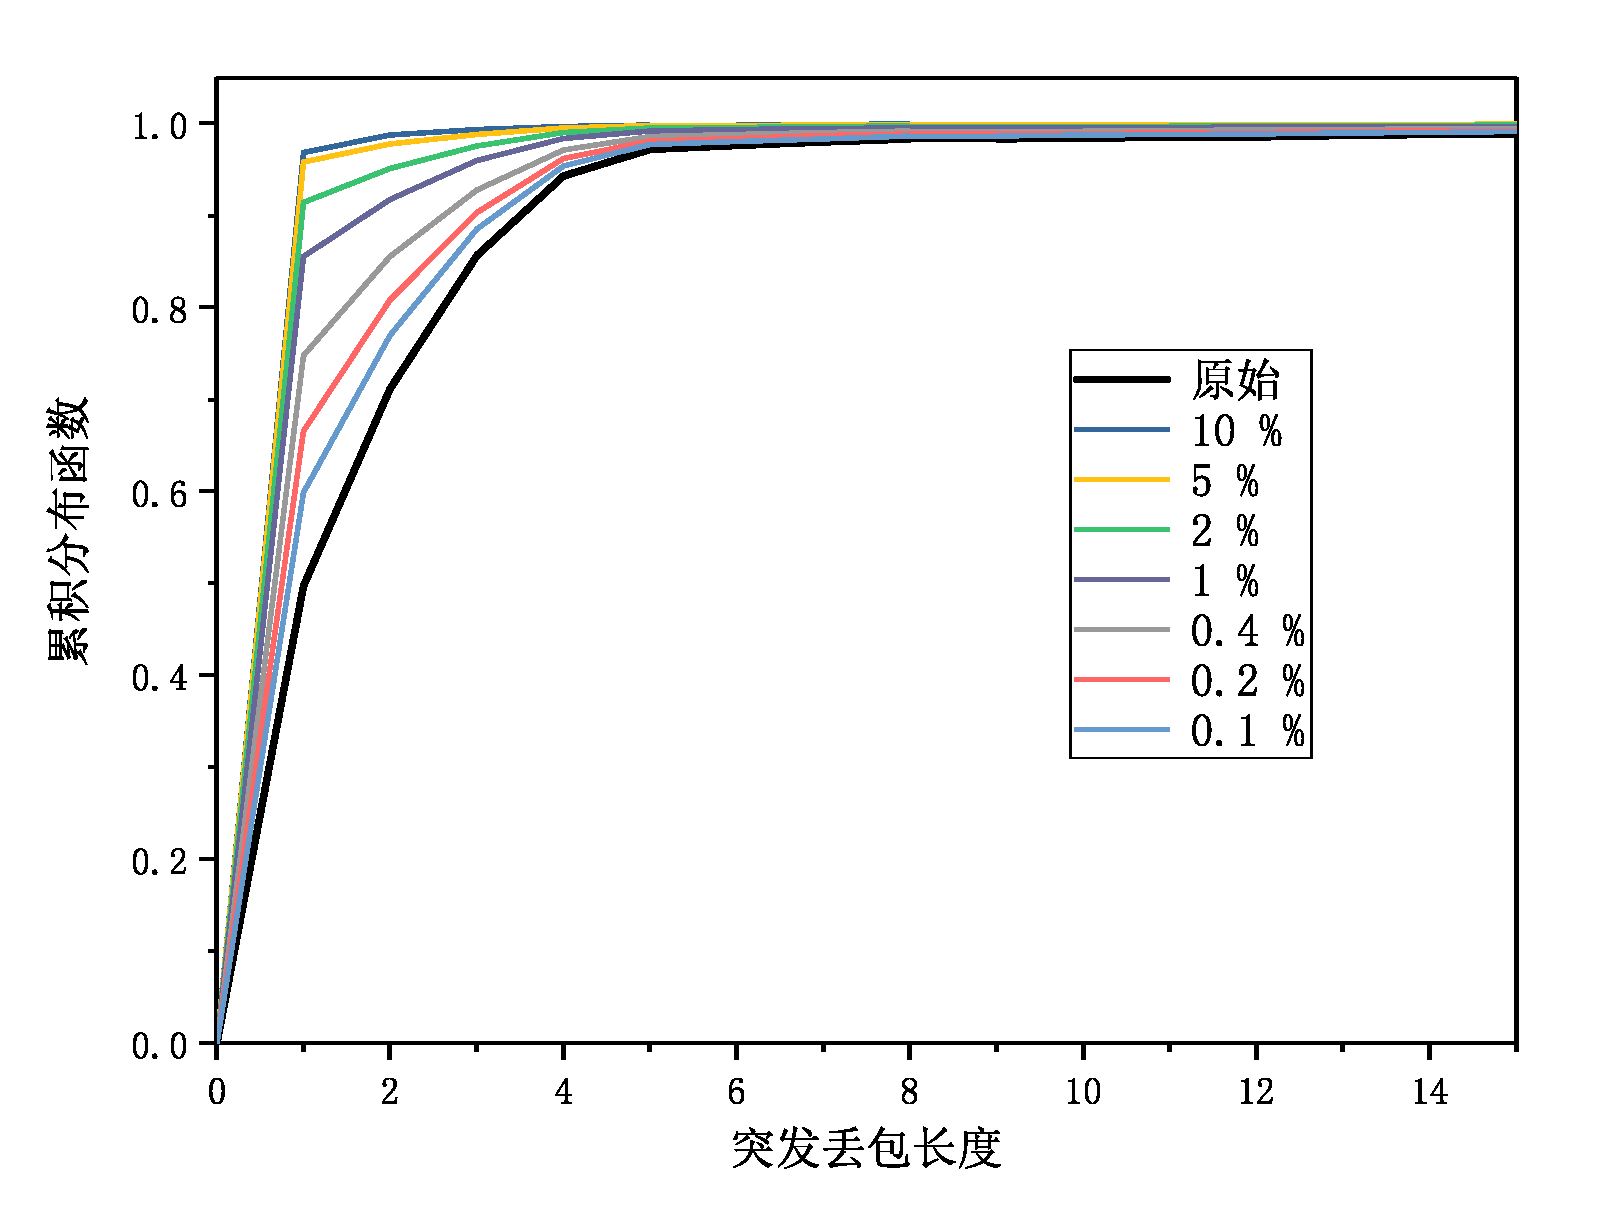
\includegraphics[width=0.48\textwidth]{chapters/chapter3/figures/burst-cdf-excellent.pdf}
        }
        \subfigure[Good场景的CDF曲线]{
            \label{fig:3:result:burst:cdf:good}
            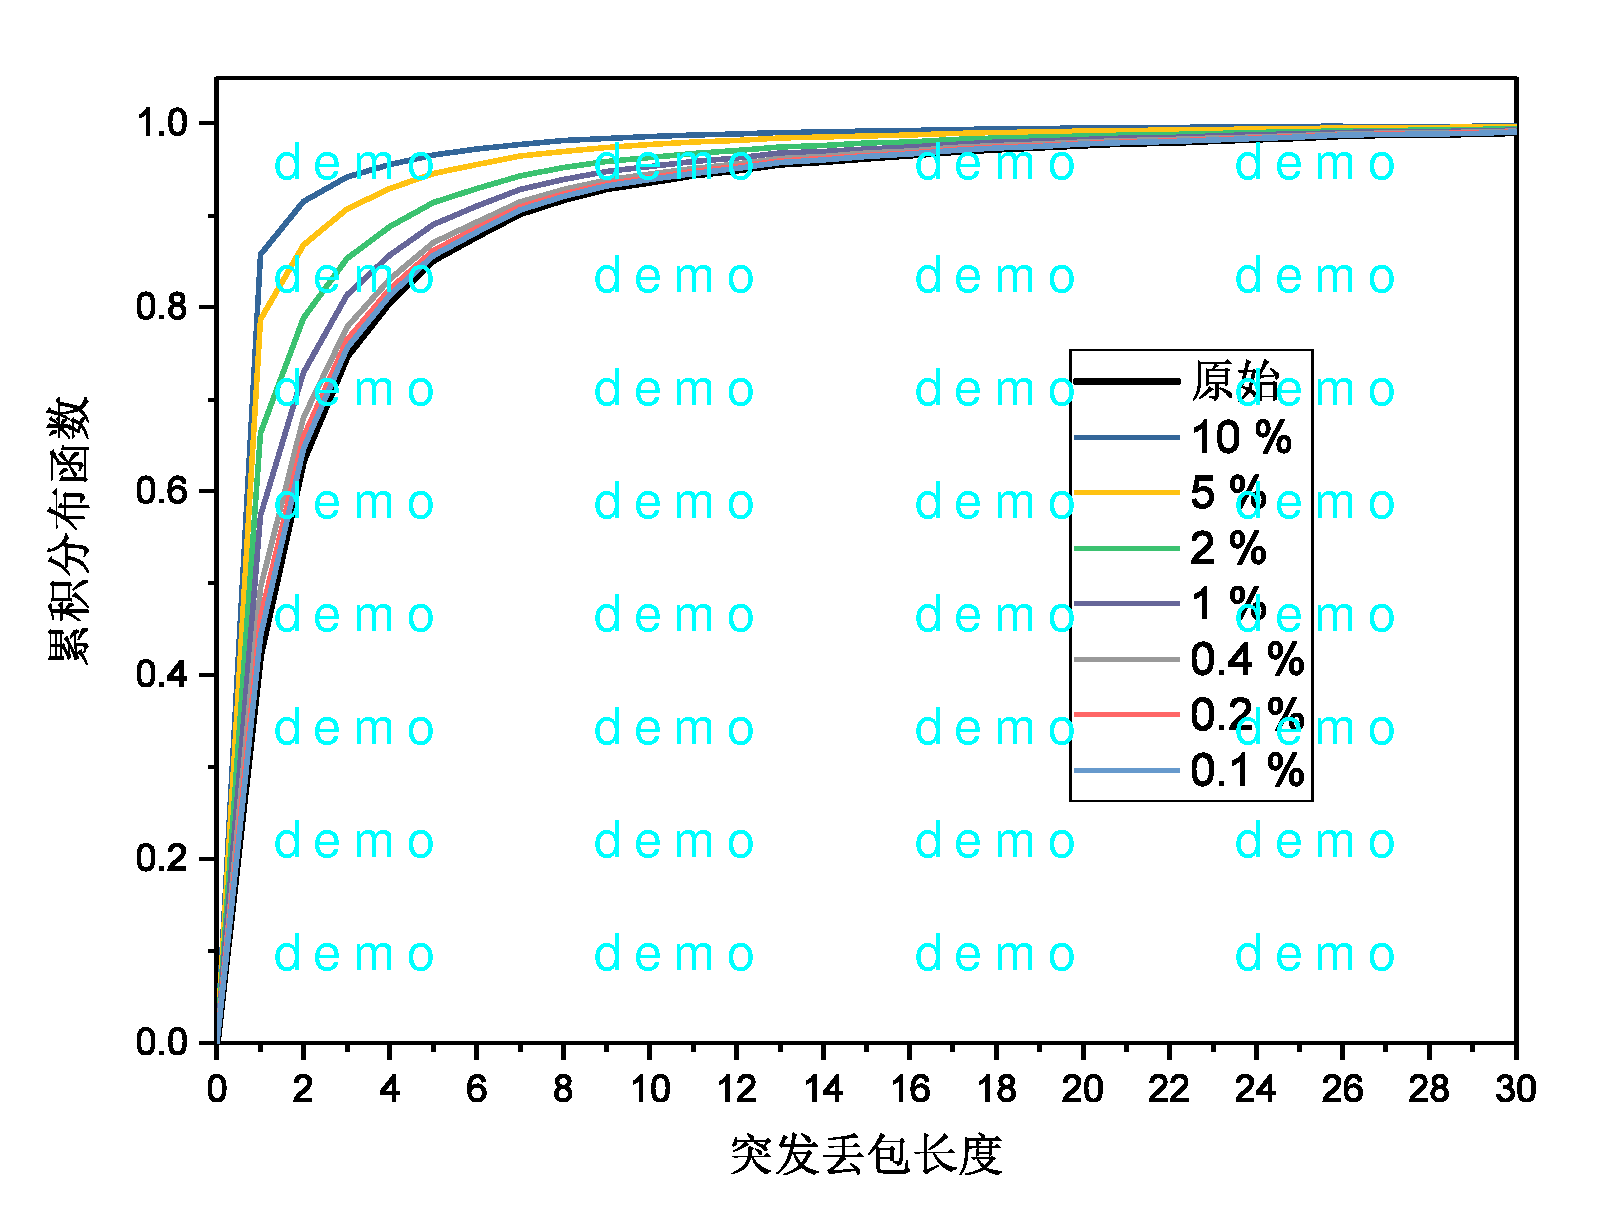
\includegraphics[width=0.48\textwidth]{chapters/chapter3/figures/burst-cdf-good.pdf}
        }
        \caption{连续丢包数的CDF曲线}
        \label{fig:3:result:burst:cdf}
	\end{figure}
}

如图\ \nref{fig:3:result:burst:cdf},时间隐通道对连续丢包数分布产生了影响。图\ \nref{fig:3:result:burst:cdf:excellent}Excellent场景中,随着主动丢包率的增加,曲线的上升趋势加快,偏离原始分布。图\ \nref{fig:3:result:burst:cdf:good}Good场景中,由于原始分布中已经存在较多的丢包,所以时间隐通道产生的影响较小,但对比原始分布,曲线上升趋势也发生改变。通过CDF判断,样本中存在时间隐通道的可能,需要进一步量化评估。

\subsubsection{条件熵检测结果}
\label{chap:analyze:result:burst:kld}

\insertFigure{
    \begin{figure}[htb]
        \centering
        \subfigure[Excellent场景K-L散度的箱线图]{
            \label{fig:3:result:burst:kld:excellent}
            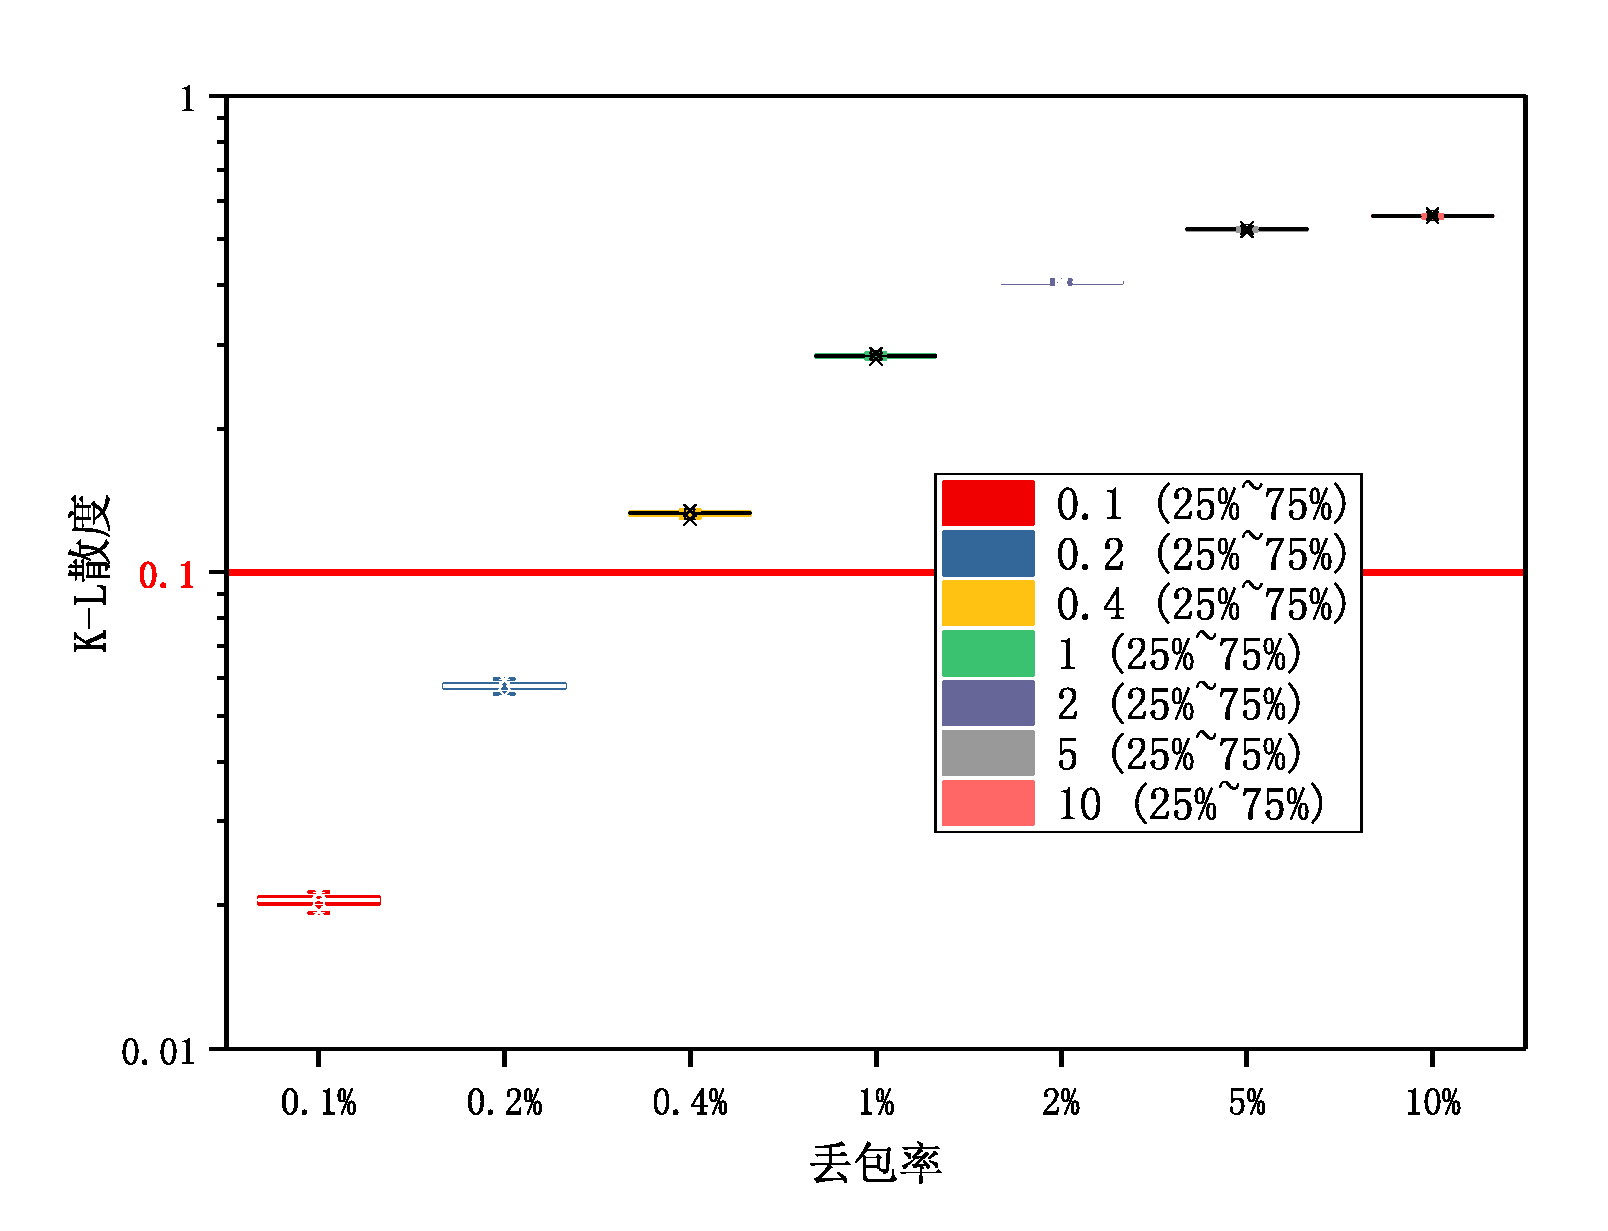
\includegraphics[width=0.48\textwidth]{chapters/chapter3/figures/burst-kld-excellent.pdf}
        }
        \subfigure[Good场景K-L散度的箱线图]{
            \label{fig:3:result:burst:kld:good}
            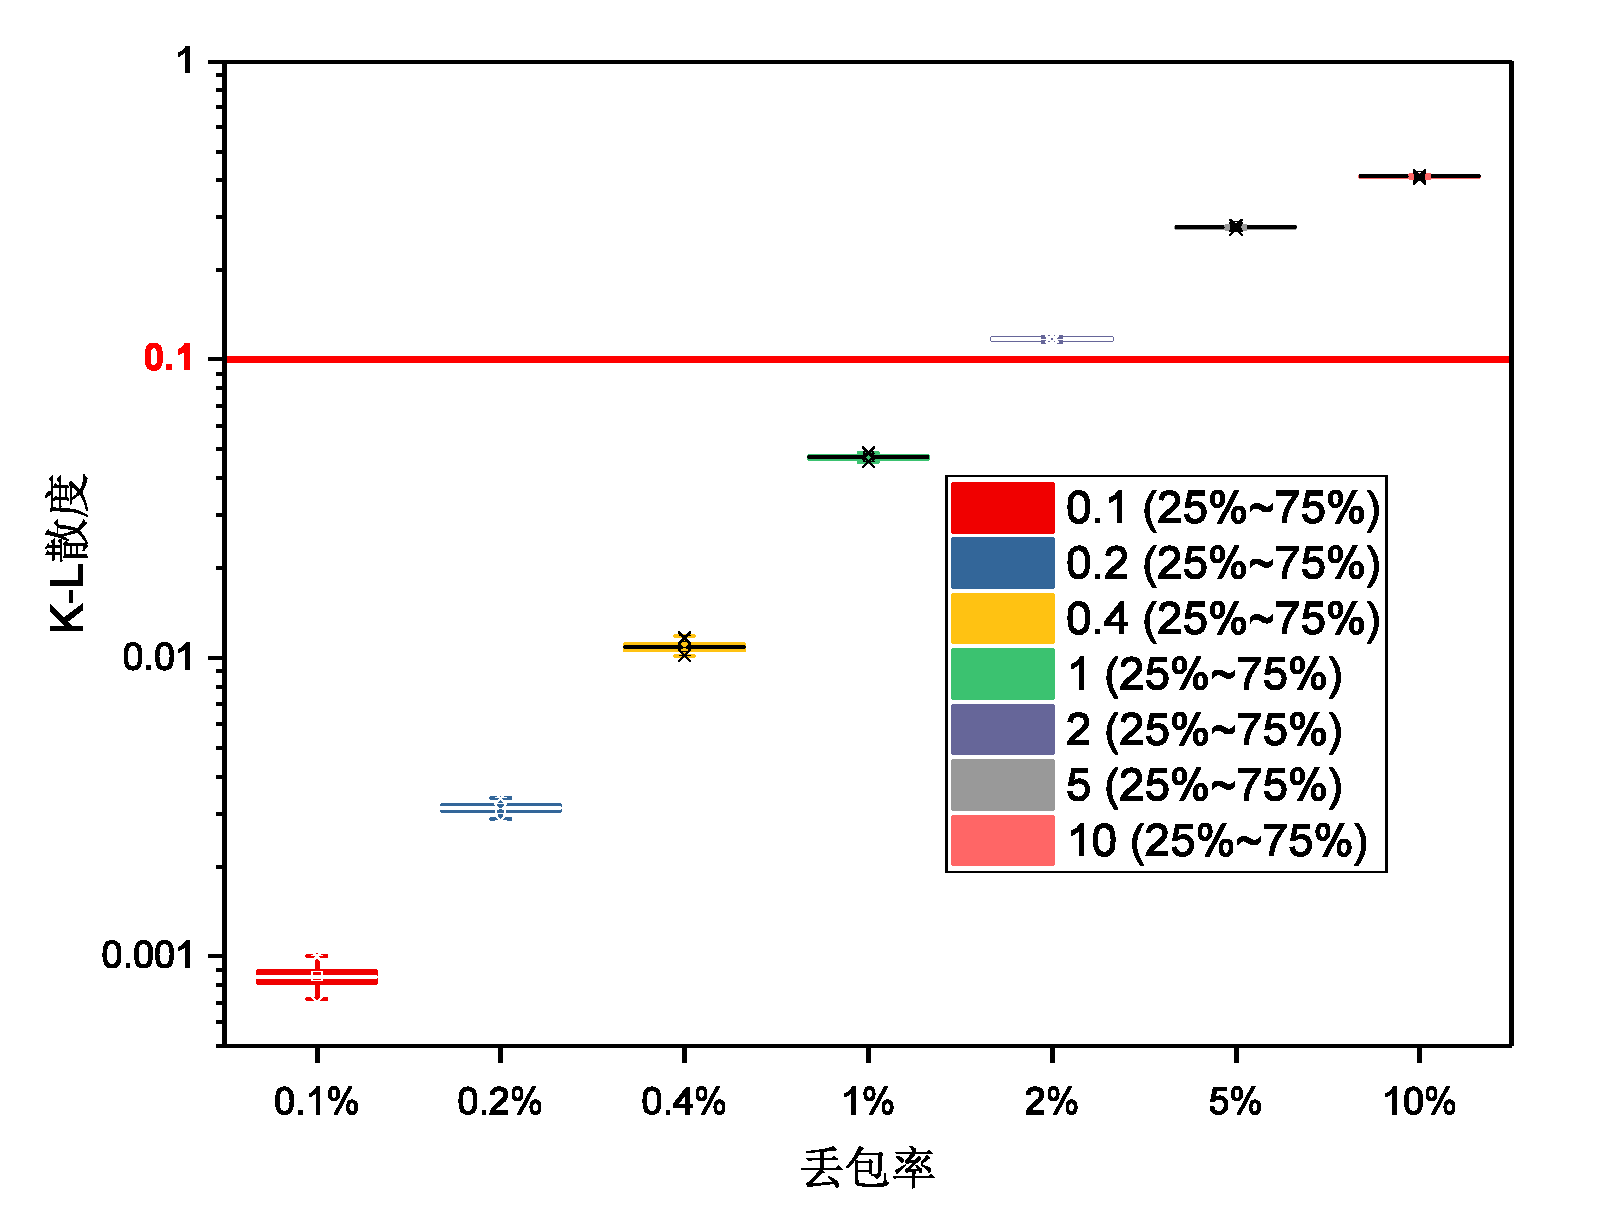
\includegraphics[width=0.48\textwidth]{chapters/chapter3/figures/burst-kld-good.pdf}
        }
        \caption{连续丢包数K-L散度检测的箱线图}
        \label{fig:3:result:burst:kld}
    \end{figure}
}

如图\ \nref{fig:3:result:burst:kld},通过K-L散度已经能够有效检测时间隐通道。图\ \nref{fig:3:result:burst:kld:excellent}Excellent场景中,只有主动丢包率$\le 0.2\ \%$时,才通过K-L散度检测。图\ \nref{fig:3:result:burst:kld:good}Good场景中,当主动丢包率$\le 1\ \%$时,即可通过K-L散度检测。检测结果表明,良好的网络条件中,对主动丢包时间隐通道的要求较高;而Good场景中,基于主动丢包的时间隐通道更容易隐蔽于网络噪声中。

\subsubsection{相对距离检测结果}
\label{chap:analyze:result:burst:distance}

\insertFigure{
	\begin{figure}[htb]
        \centering
        \subfigure[Excellent场景Wasserstein距离的箱线图]{
            \label{fig:3:result:burst:wd:excellent}
            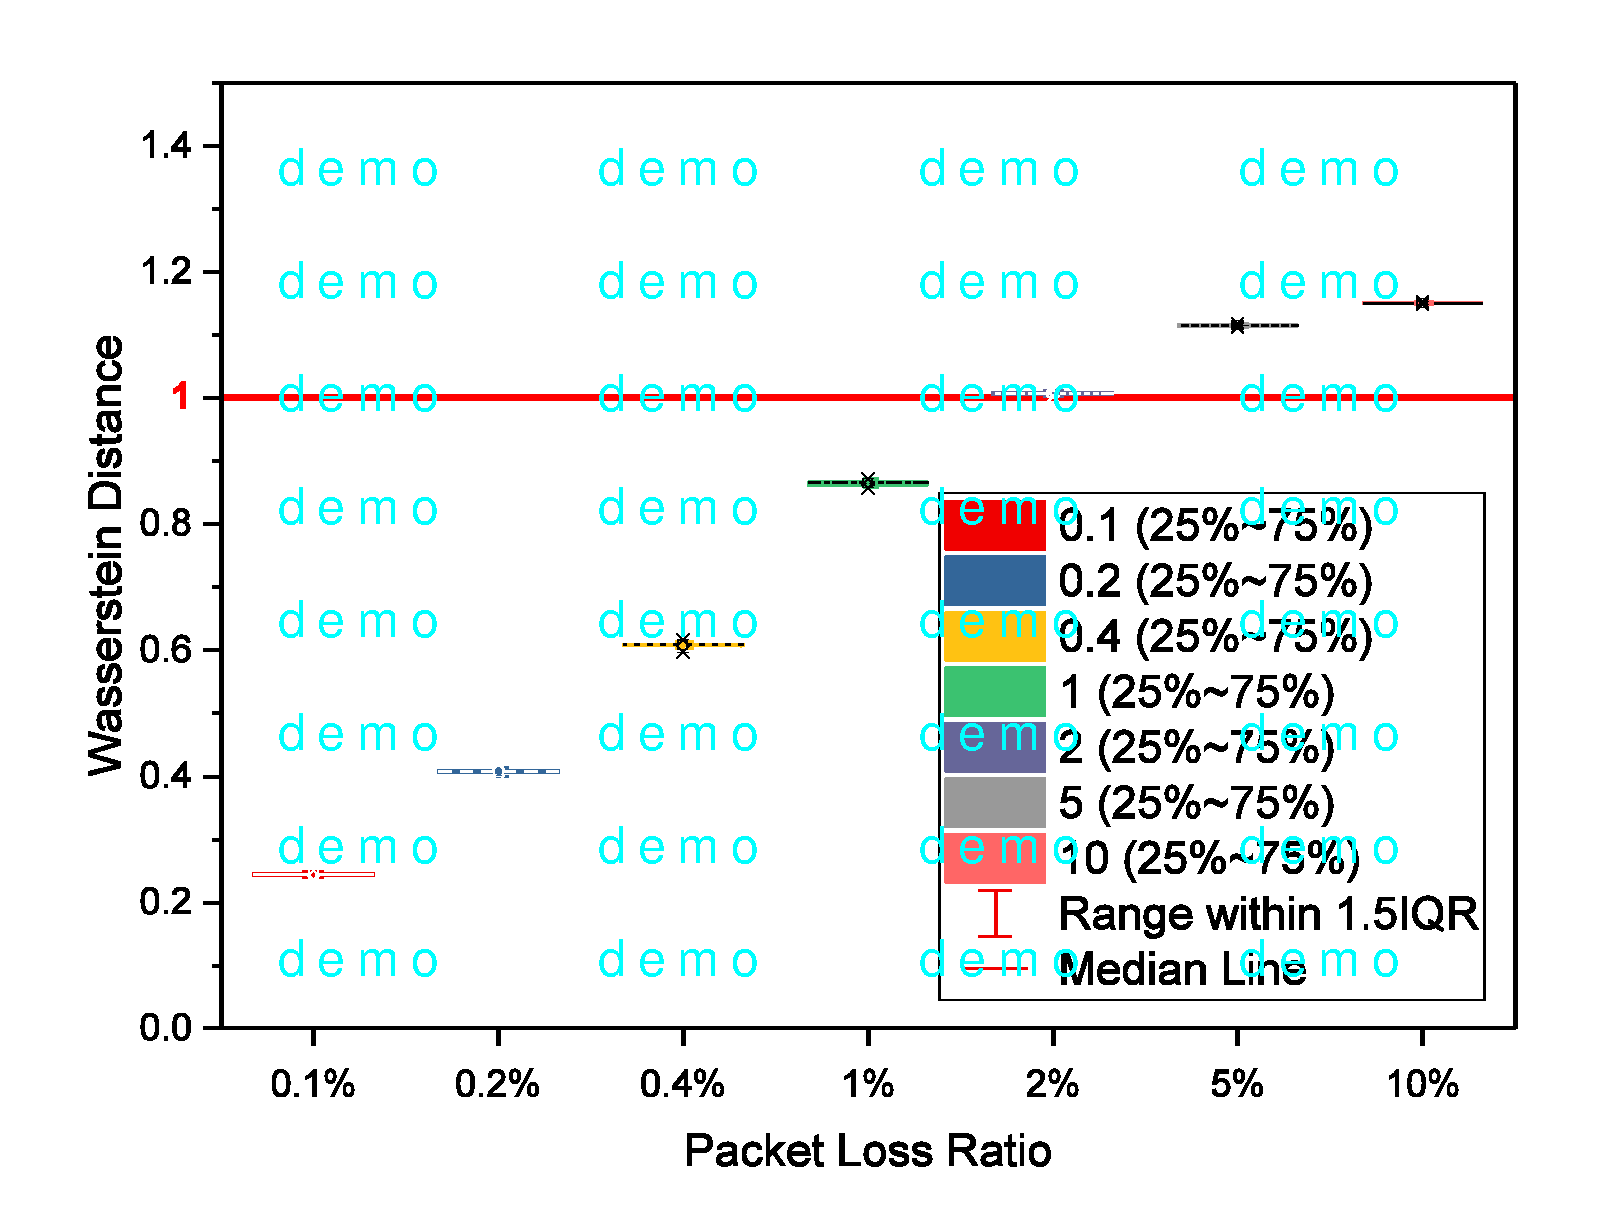
\includegraphics[width=0.48\textwidth]{chapters/chapter3/figures/burst-wd-excellent.pdf}
        }
        \subfigure[Good场景Wasserstein距离的箱线图]{
            \label{fig:3:result:burst:wd:good}
            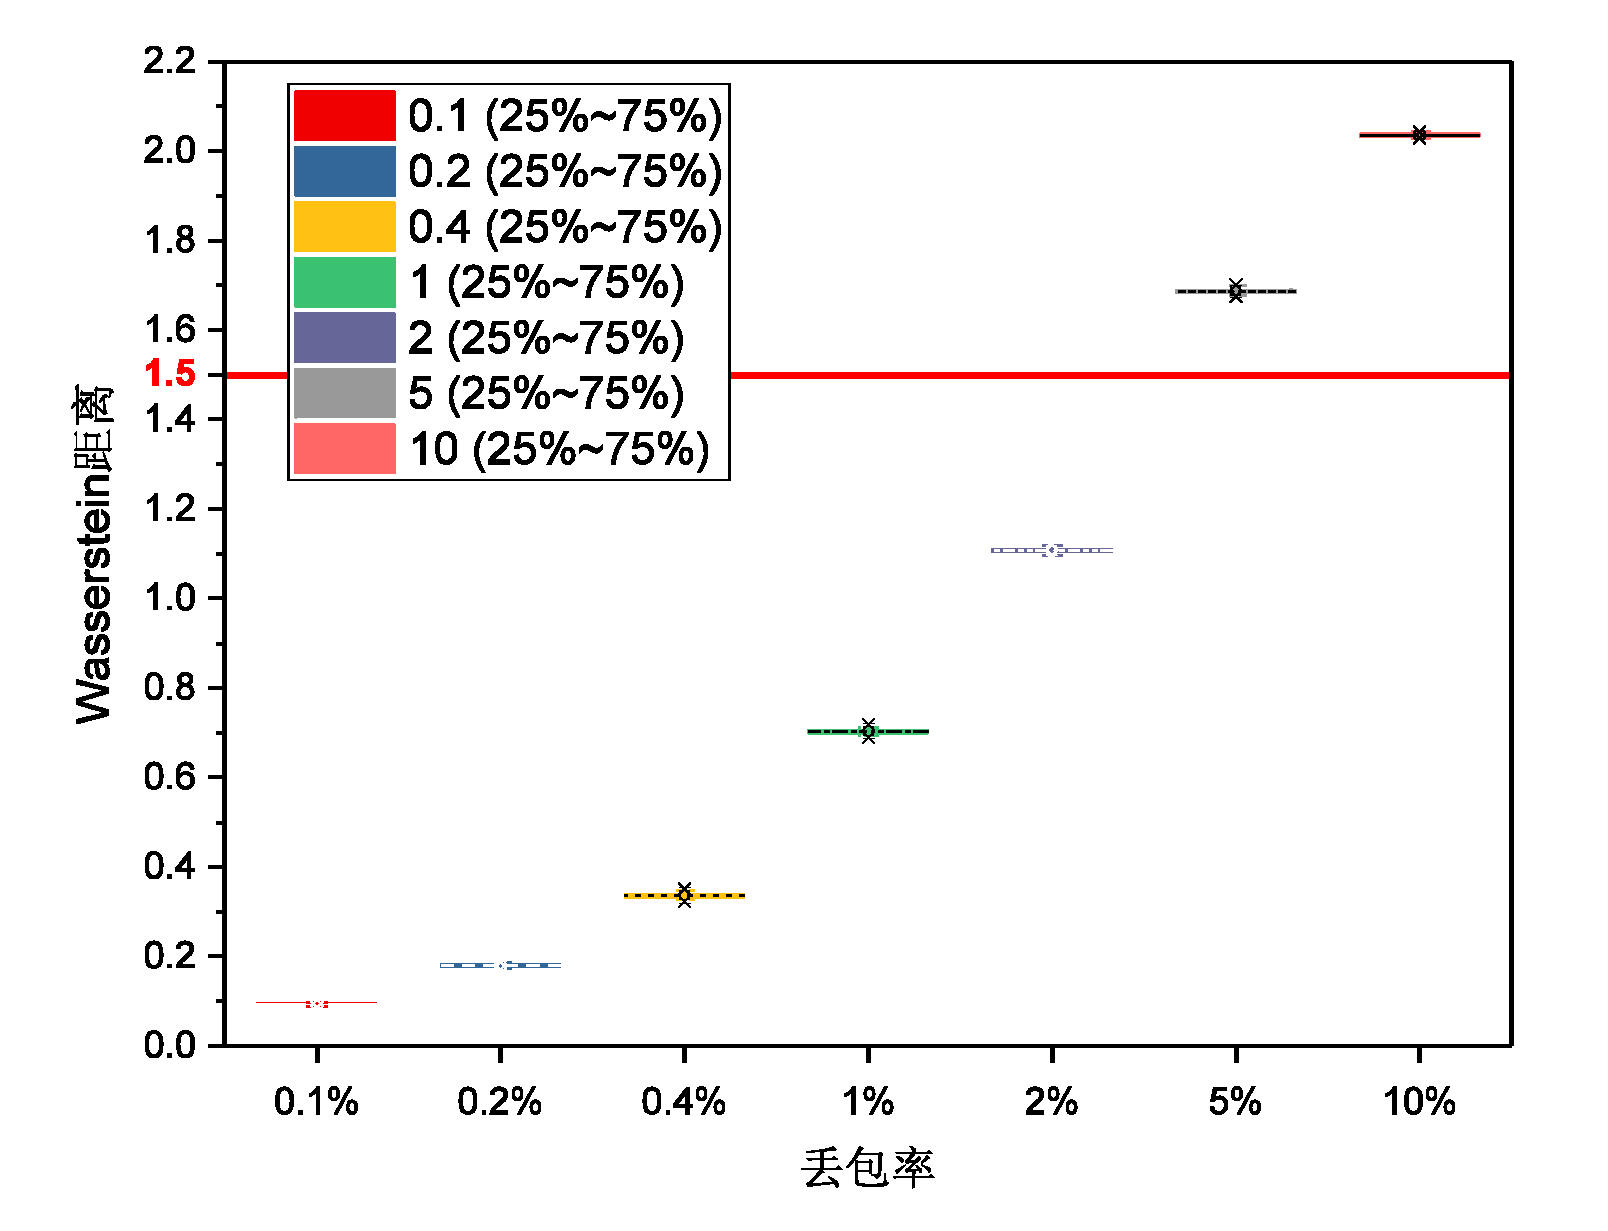
\includegraphics[width=0.48\textwidth]{chapters/chapter3/figures/burst-wd-good.pdf}
        }
        \caption{连续丢包数Wasserstein距离检测的箱线图}
        \label{fig:3:result:burst:wd}
	\end{figure}

	\begin{figure}[htb]
        \centering
        \subfigure[Excellent场景能量距离的箱线图]{
            \label{fig:3:result:burst:ed:excellent}
            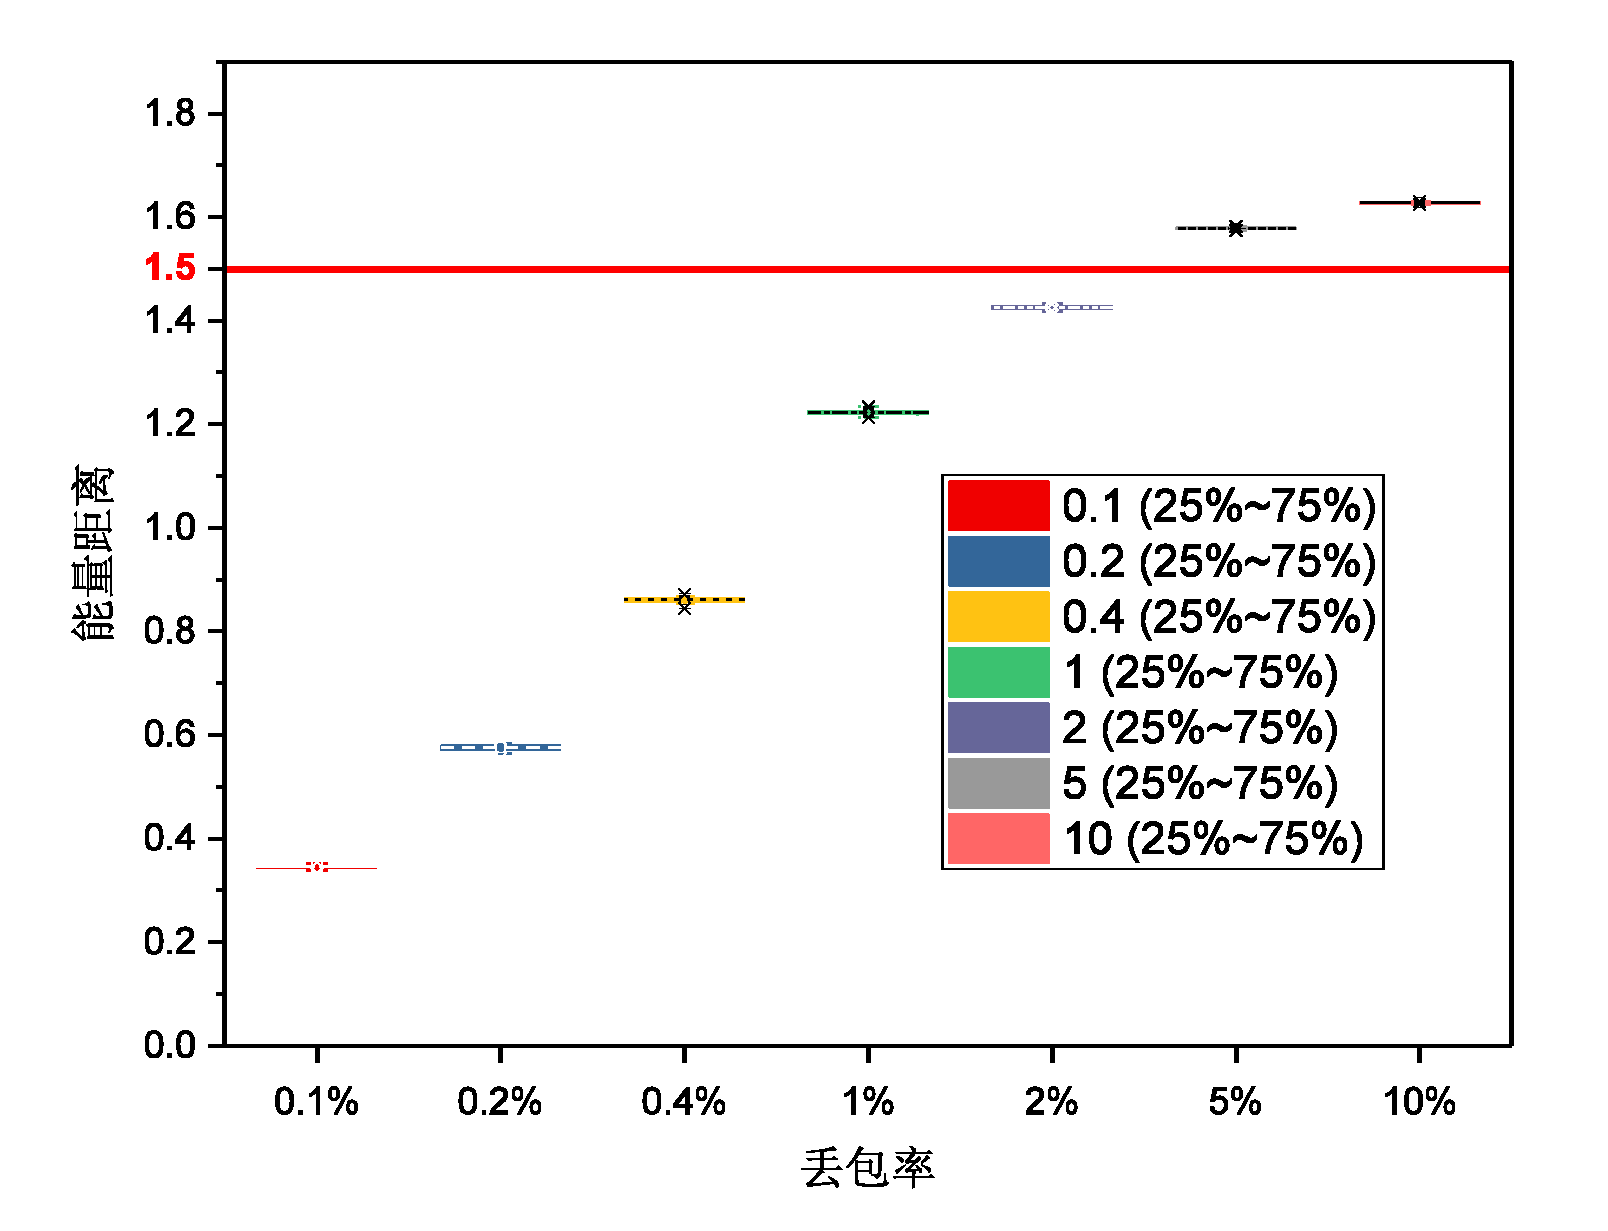
\includegraphics[width=0.48\textwidth]{chapters/chapter3/figures/burst-ed-excellent.pdf}
        }
        \subfigure[Good场景能量距离的箱线图]{
            \label{fig:3:result:burst:ed:good}
            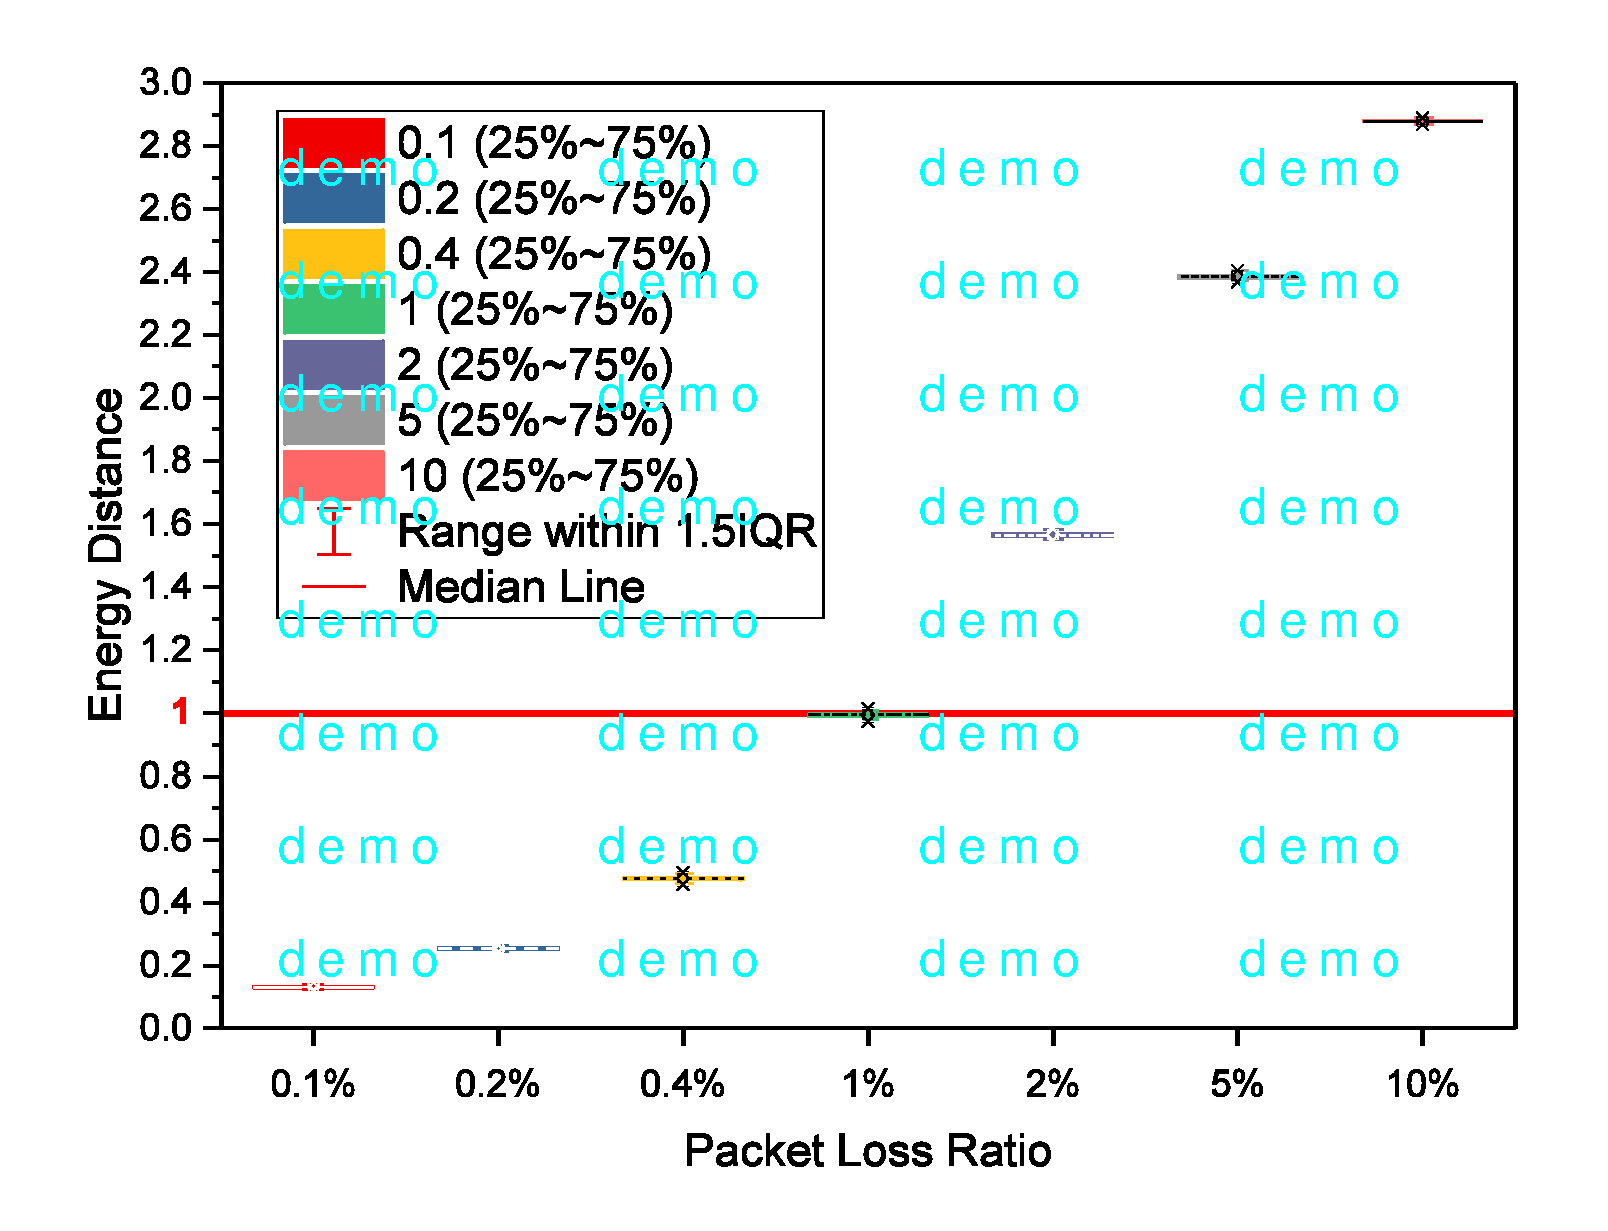
\includegraphics[width=0.48\textwidth]{chapters/chapter3/figures/burst-ed-good.pdf}
        }
        \caption{连续丢包数能量距离检测的箱线图}
        \label{fig:3:result:burst:ed}
	\end{figure}
}

如图\ \nref{fig:3:result:burst:wd},两种场景下Wasserstein距离检测结果总体一致。Excellent场景中,主动丢包率$\le 10\ \%$即可通过Wasserstein距离检测;而Good场景中,主动丢包率$\le 2\ \%$才通过检测。由于时间隐通道产生的连续丢包数为1,因此Good场景中的累积效应影响较大。

如图\ \nref{fig:3:result:burst:ed},能量距离检测结果与Wasserstein距离检测结果类似。Excellent场景下,主动丢包率$\le 2\ \%$即可通过检验;Good场景下,主动丢包率$\le 1\ \%$才通过检验。能量距离检测要求较Wasserstein更加严格,Good场景较Excellent场景更加严格。在相对距离检测中,检测结果具有较好区分度,并且与CDF曲线趋势一致,表明具有较好的检测能力。

对比本文\ \nref{chap:analyze:result:ipd}基于IPD的检测结果,基于连续丢包数分布的检测,已能能够有效检测基于主动丢包的时间隐通道。Excellent场景下,K-L散度具有更好的检测效果;Good场景下,相对距离检测的效果优于K-L散度检测。

\subsection{区间丢包数检测结果评估}
\label{chap:analyze:result:window}

如图\ \nref{fig:3:capture:win-cdf},不同区间长度设定下,区间丢包数随之变化。较小的区间长度有益于Excellent场景的检测,较大的区间长度有益于Good场景的检测。本检测中,区间长度设定为100及200。

\subsubsection{CDF检测结果}
\label{chap:analyze:result:window:cdf}

\insertFigure{
    \begin{figure}[htbp]
        \centering
        \subfigure[区间长度为100时Excellent场景的CDF曲线]{
            \label{fig:3:result:win100:cdf:excellent}
            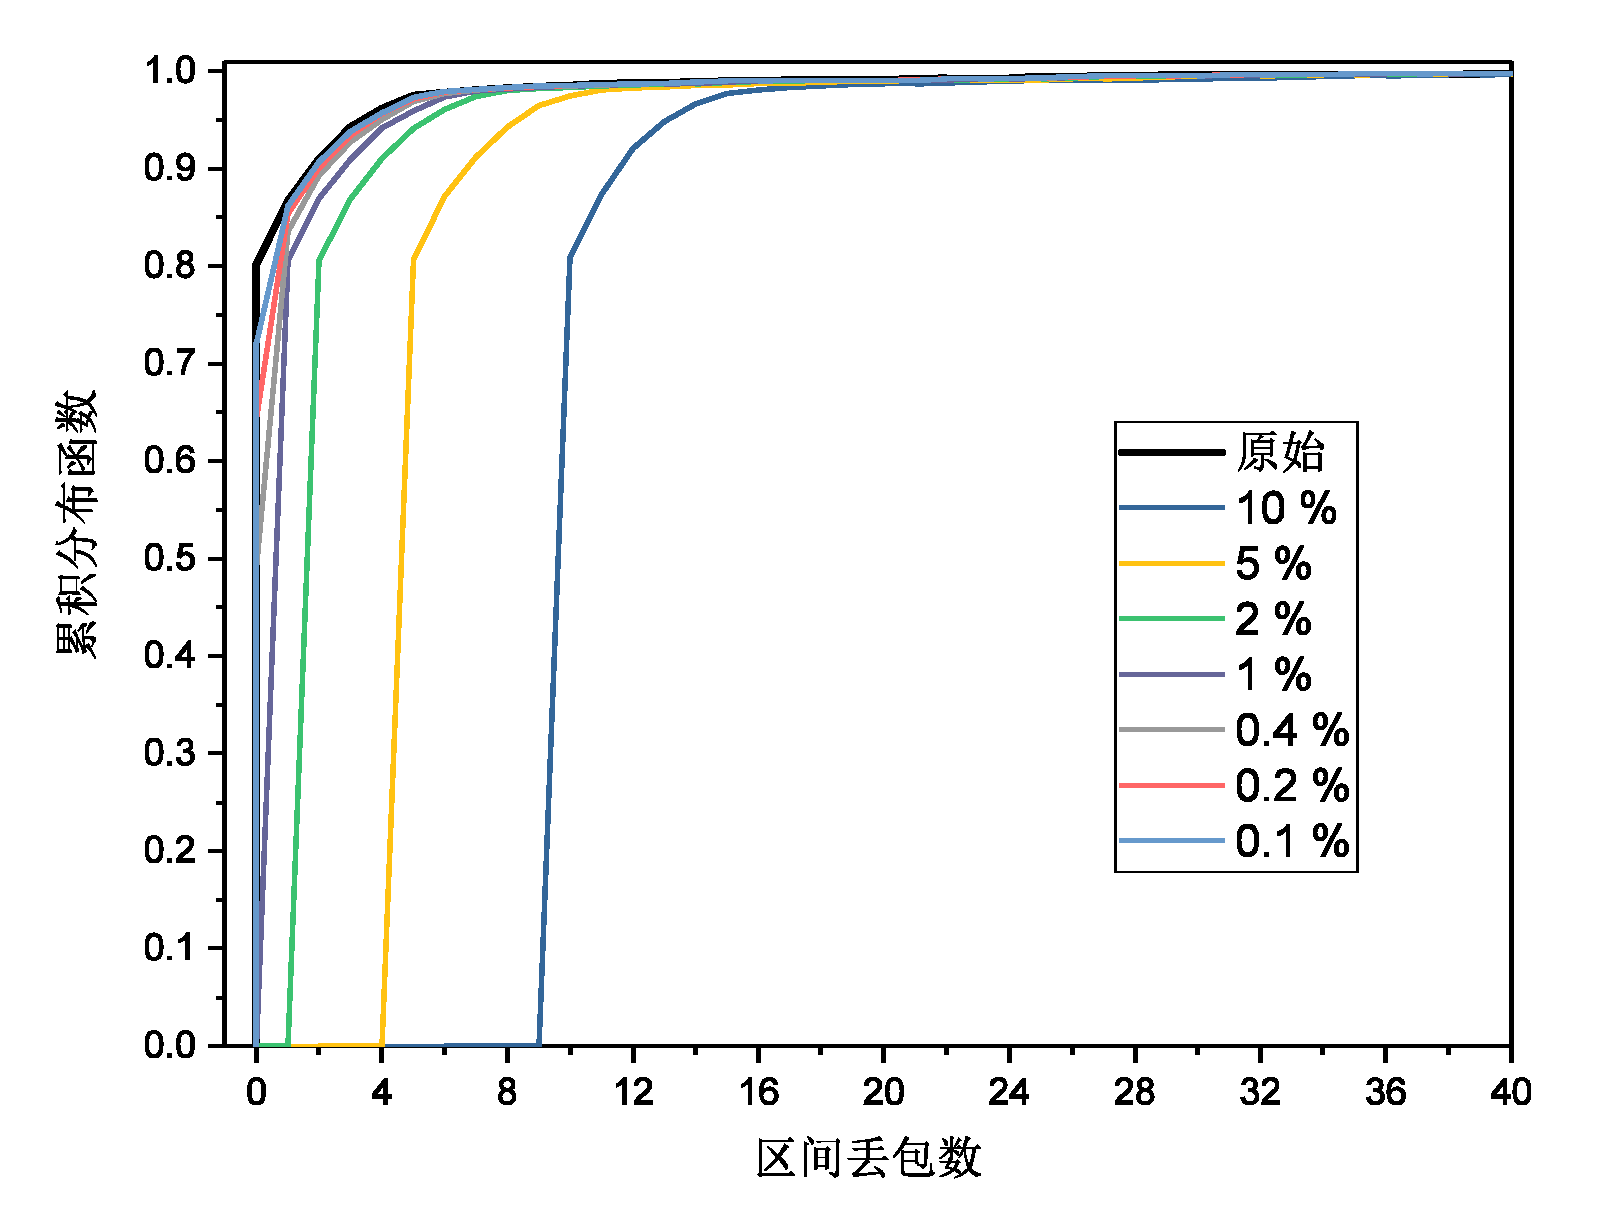
\includegraphics[width=0.48\textwidth]{chapters/chapter3/figures/win100-cdf-excellent.pdf}
        }
        \subfigure[区间长度为100时Good场景的CDF曲线]{
            \label{fig:3:result:win100:cdf:good}
            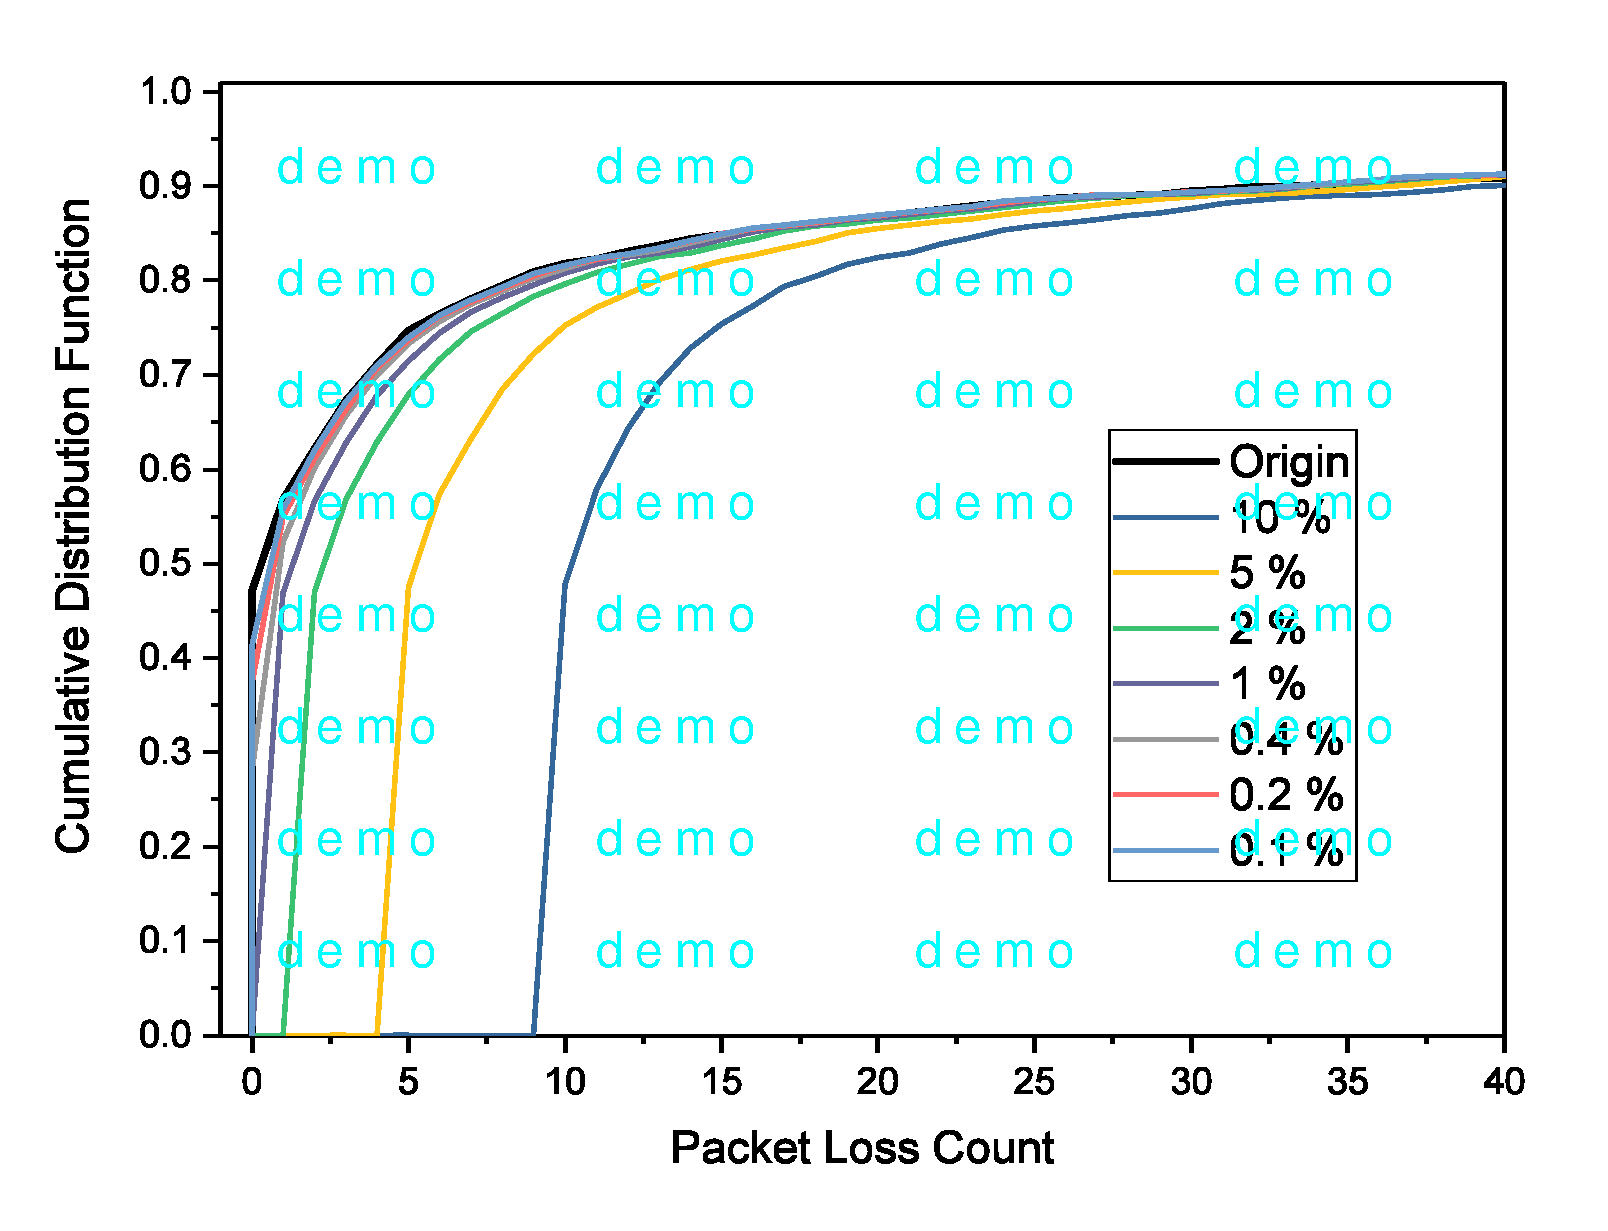
\includegraphics[width=0.48\textwidth]{chapters/chapter3/figures/win100-cdf-good.pdf}
        }
        \subfigure[区间长度为200时Excellent场景的CDF曲线]{
            \label{fig:3:result:win200:cdf:excellent}
            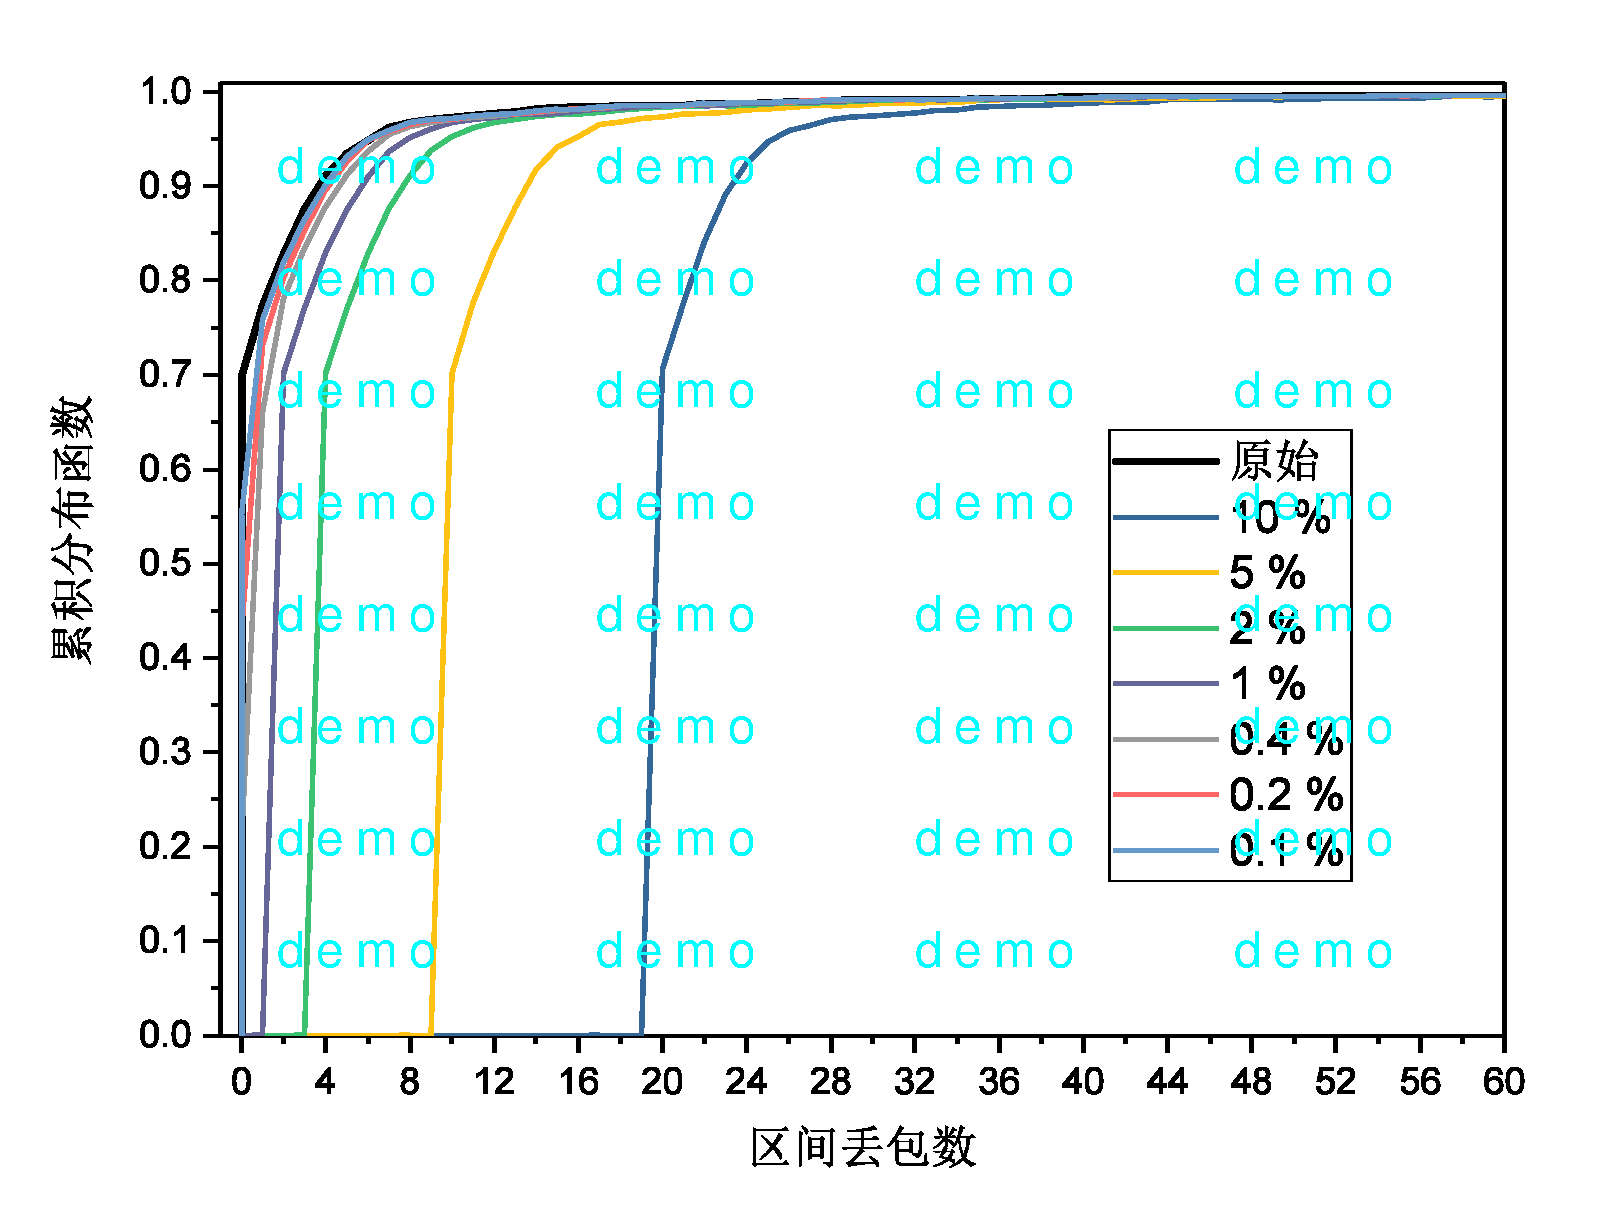
\includegraphics[width=0.48\textwidth]{chapters/chapter3/figures/win200-cdf-excellent.pdf}
        }
        \subfigure[区间长度为200时Good场景的CDF曲线]{
            \label{fig:3:result:win200:cdf:good}
            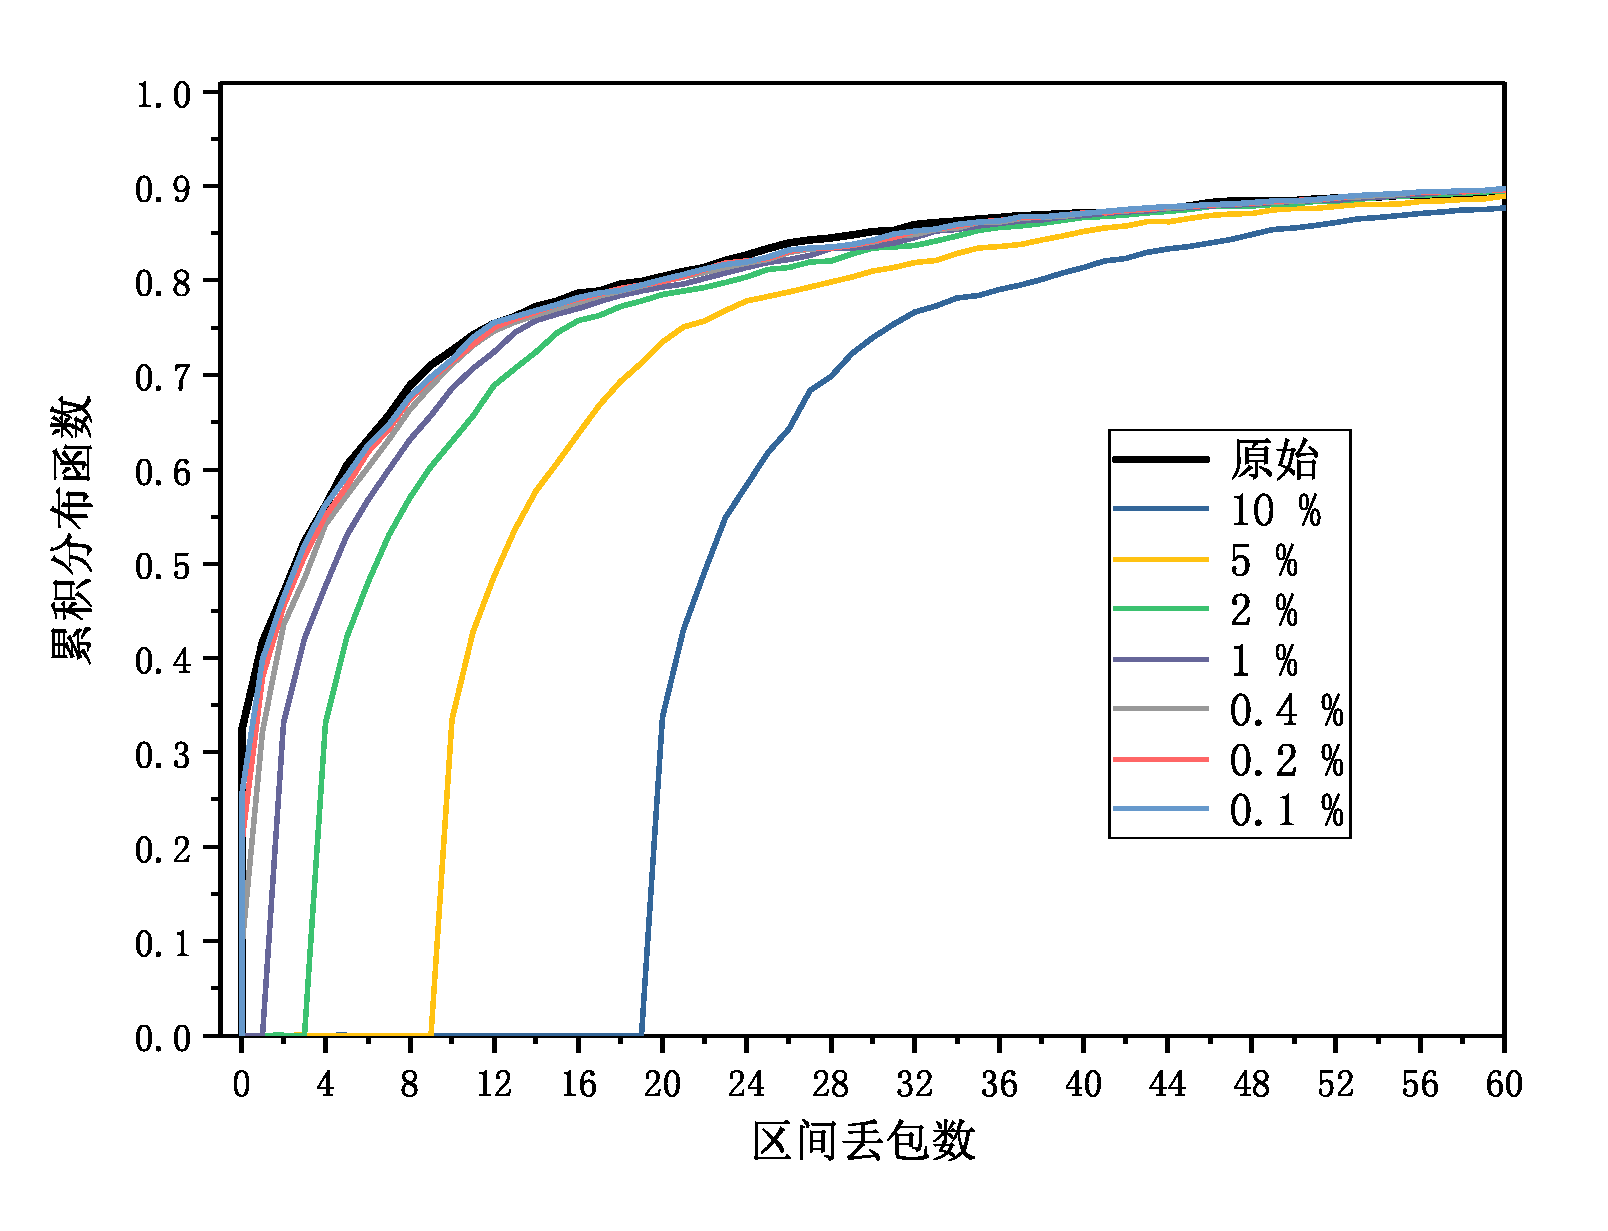
\includegraphics[width=0.48\textwidth]{chapters/chapter3/figures/win200-cdf-good.pdf}
        }
        \caption{区间丢包数的CDF曲线}
        \label{fig:3:result:win:cdf}
	\end{figure}
}

如图\ \nref{fig:3:result:win:cdf},时间隐通道对CDF曲线产生了影响。对比图\ \nref{fig:3:result:win100:cdf:excellent}及图\ \nref{fig:3:result:win100:cdf:good},区间长度相同时,Excellent场景下的CDF曲线上升趋势更加迅速,意味着丢包数较少的区间占据的比例较高。对比图\ \nref{fig:3:result:win100:cdf:excellent}及图\ \nref{fig:3:result:win200:cdf:excellent},相同场景中增大区间长度后,曲线的上升趋势减缓,更有利于判断分布的差异。

对比CDF曲线,时间隐通道的主动丢包率越高,对分布曲线的影响越大。当主动丢包的间隔小于区间长度时,无丢包区间减少,CDF曲线中体现为起始位置偏移。因此,CDF曲线能够检测出主动丢包率$\ge 5\ \%$的时间隐通道。

\subsubsection{相对距离检测结果}
\label{chap:analyze:result:window:distance}

\insertFigure{
	\begin{figure}[htbp]
        \centering
        \subfigure[区间长度为100时Excellent场景的Wasserstein距离]{
            \label{fig:3:result:win100:wd:excellent}
            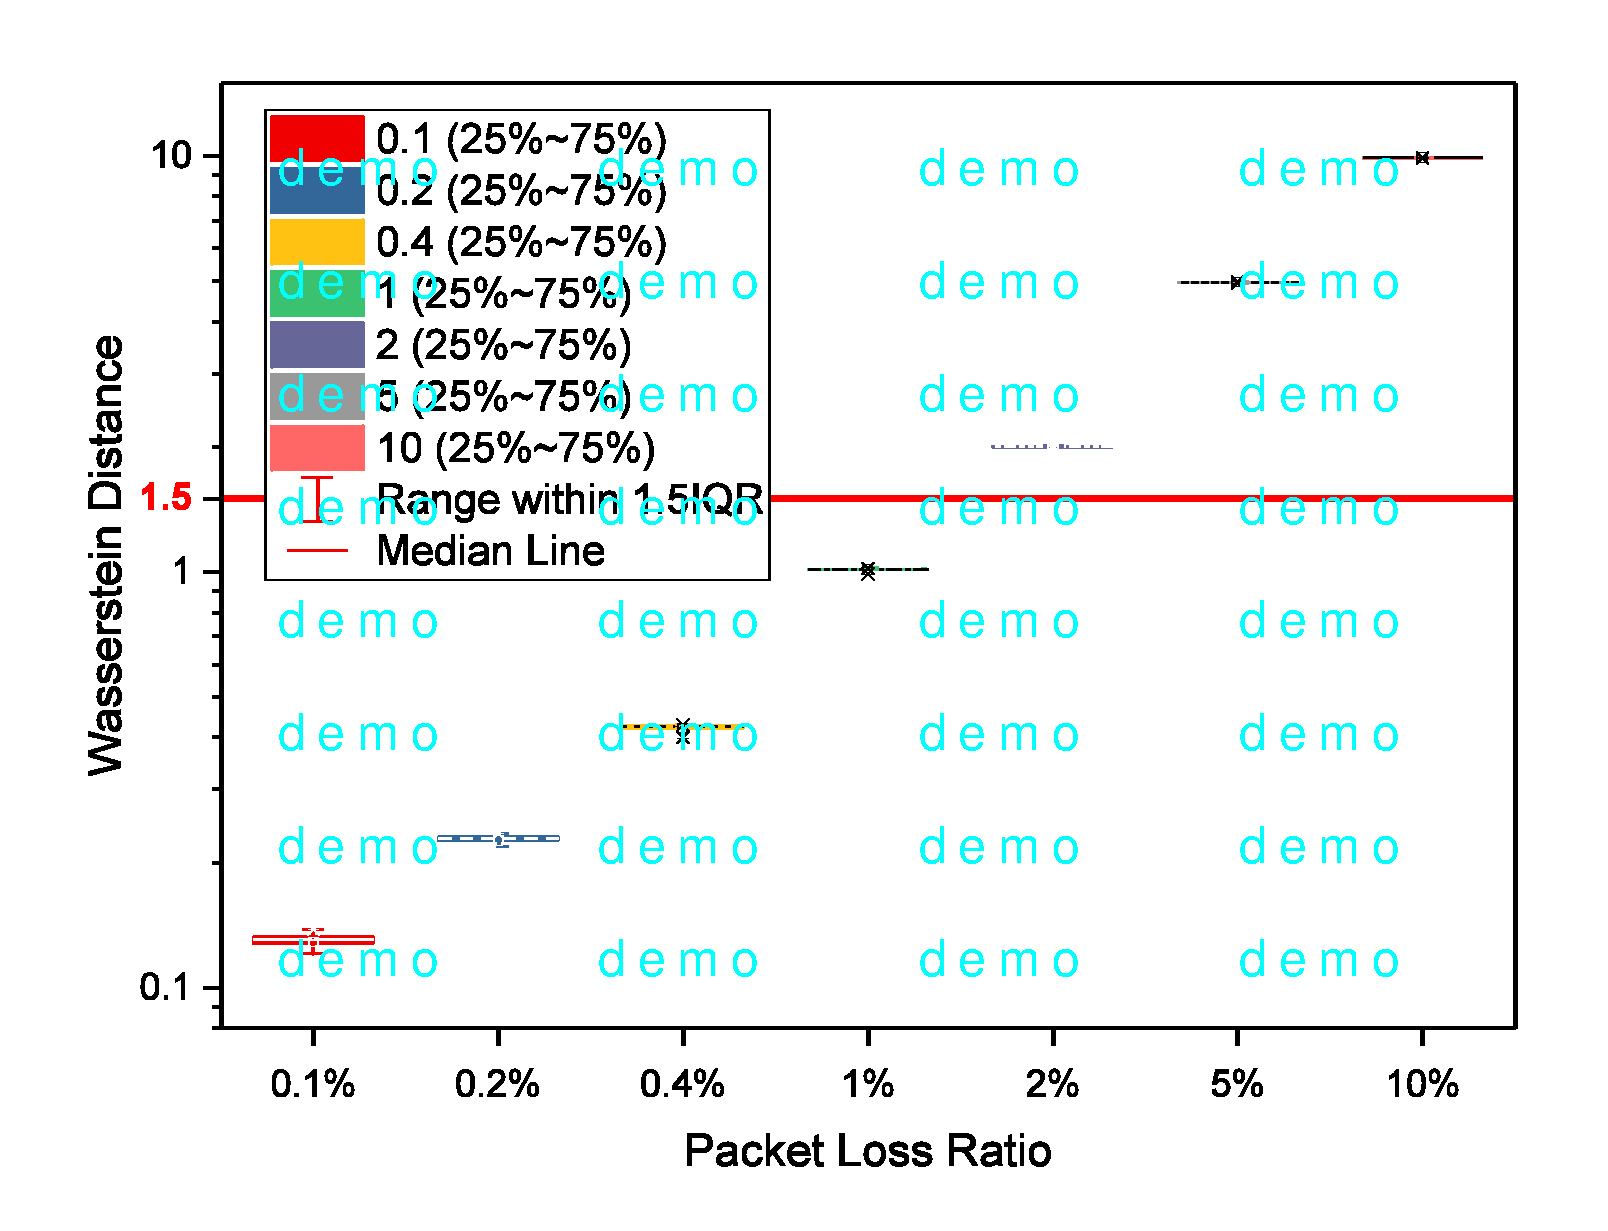
\includegraphics[width=0.48\textwidth]{chapters/chapter3/figures/win100-wd-excellent.pdf}
        }
        \subfigure[区间长度为100时Good场景的Wasserstein距离]{
            \label{fig:3:result:win100-wd:good}
            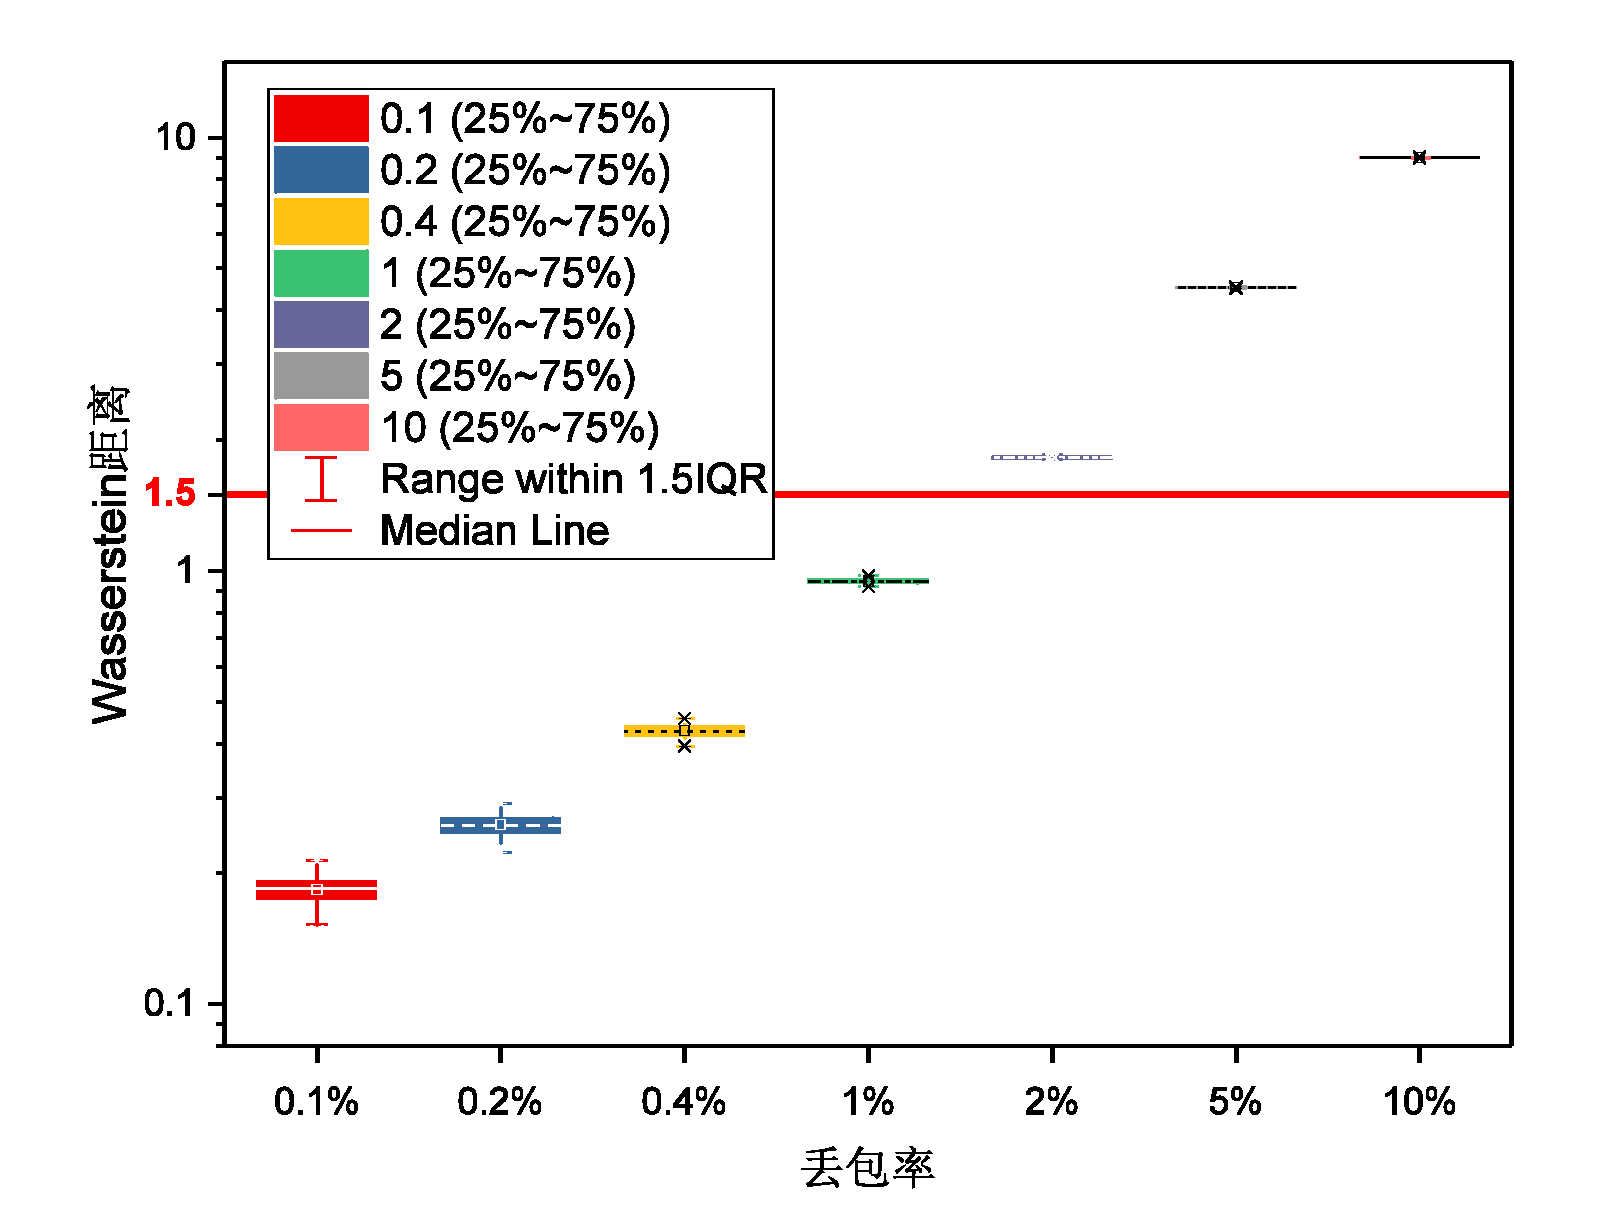
\includegraphics[width=0.48\textwidth]{chapters/chapter3/figures/win100-wd-good.pdf}
        }
        \subfigure[区间长度为200时Excellent场景的Wasserstein距离]{
            \label{fig:3:result:win200:wd:excellent}
            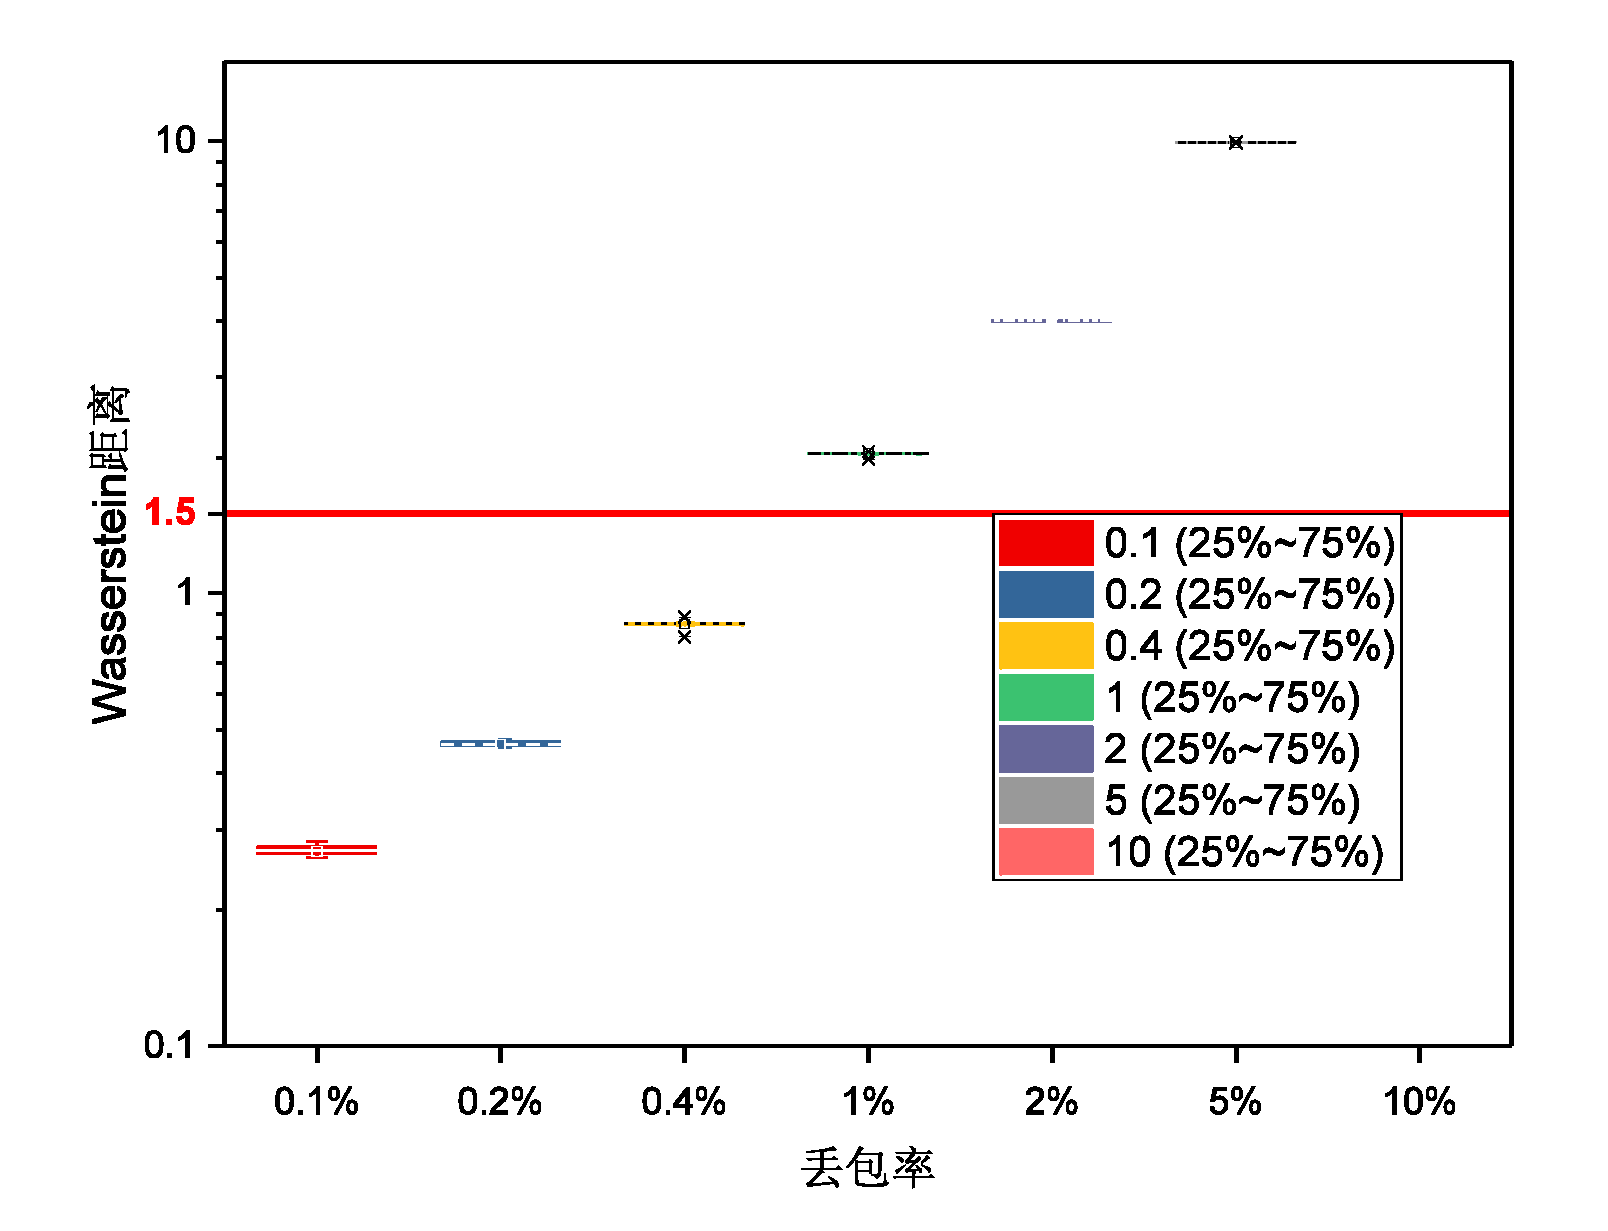
\includegraphics[width=0.48\textwidth]{chapters/chapter3/figures/win200-wd-excellent.pdf}
        }
        \subfigure[区间长度为200时Good场景的Wasserstein距离]{
            \label{fig:3:result:win200:wd:good}
            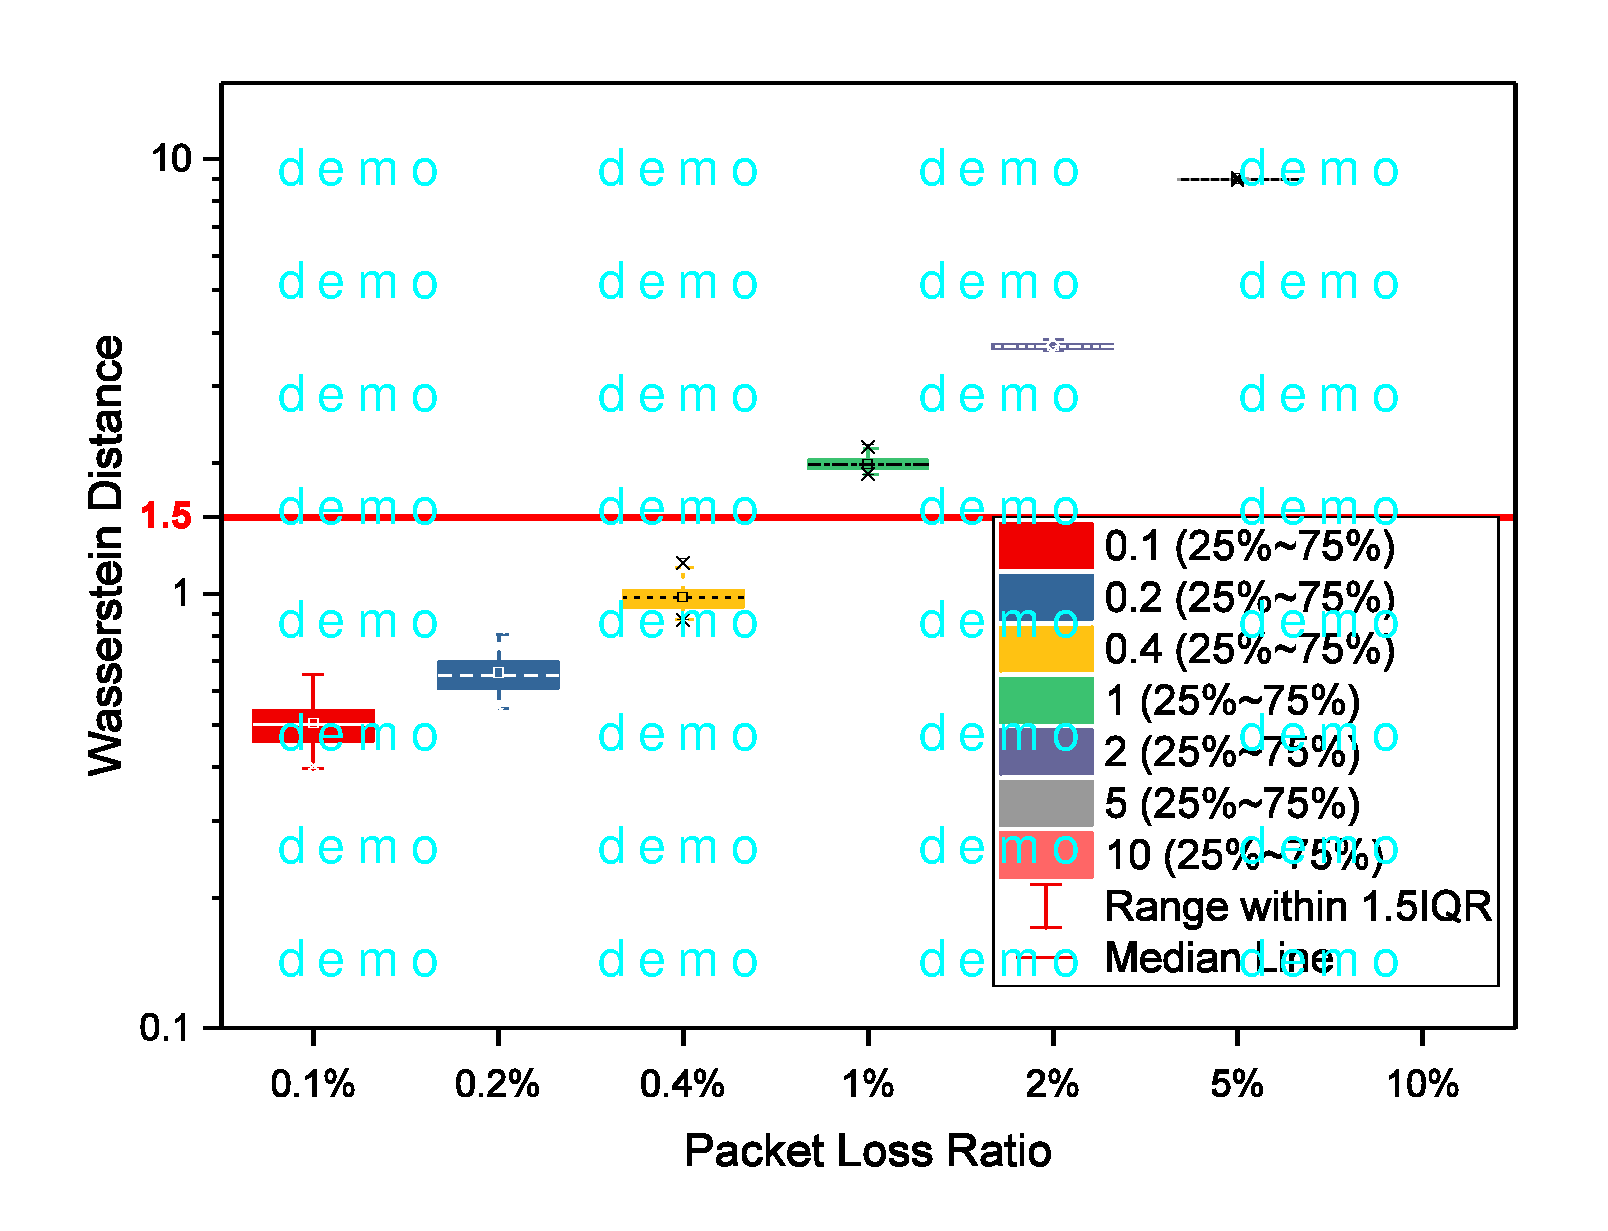
\includegraphics[width=0.48\textwidth]{chapters/chapter3/figures/win200-wd-good.pdf}
        }
        \caption{区间丢包数Wasserstein距离检测的箱线图}
        \label{fig:3:result:win:wd}
	\end{figure}

	\begin{figure}[htbp]
        \centering
        \subfigure[区间长度为100时Excellent场景能量距离的箱线图]{
            \label{fig:3:result:win100:ed:excellent}
            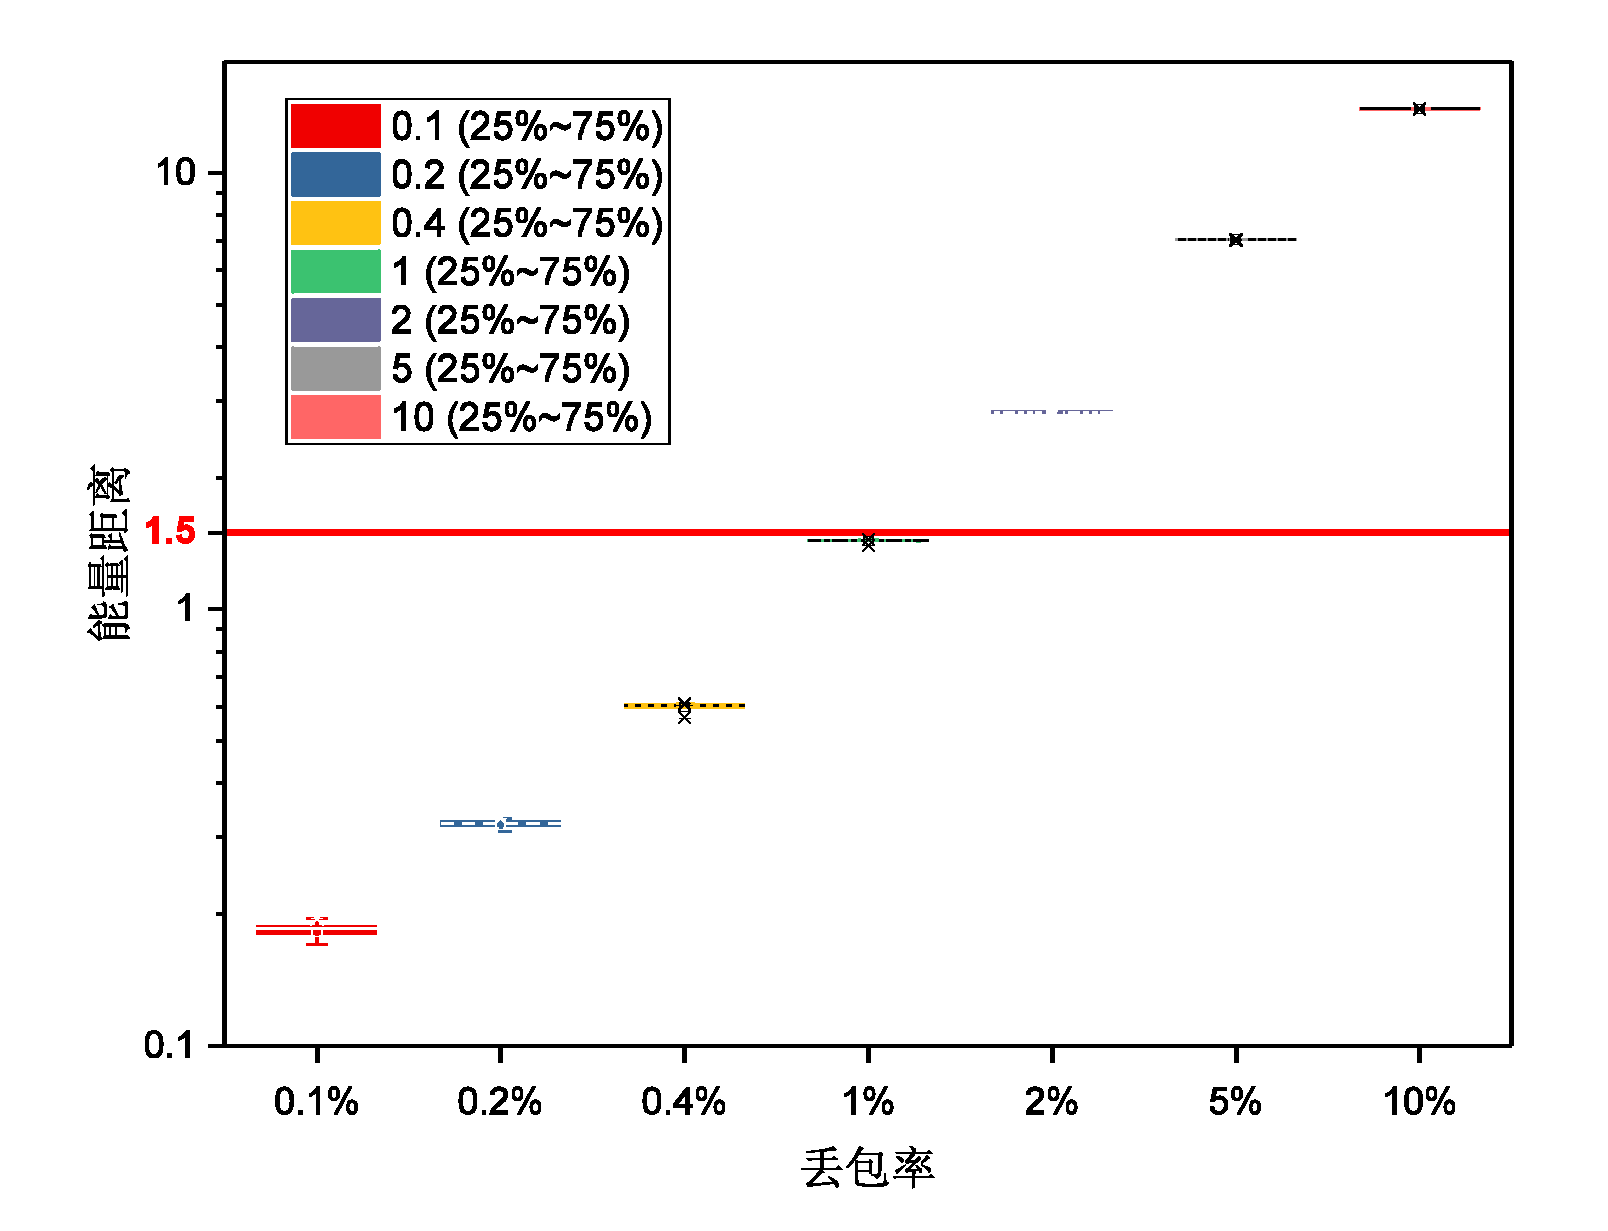
\includegraphics[width=0.48\textwidth]{chapters/chapter3/figures/win100-ed-excellent.pdf}
        }
        \subfigure[区间长度为100时Good场景能量距离的箱线图]{
            \label{fig:3:result:win100-ed:good}
            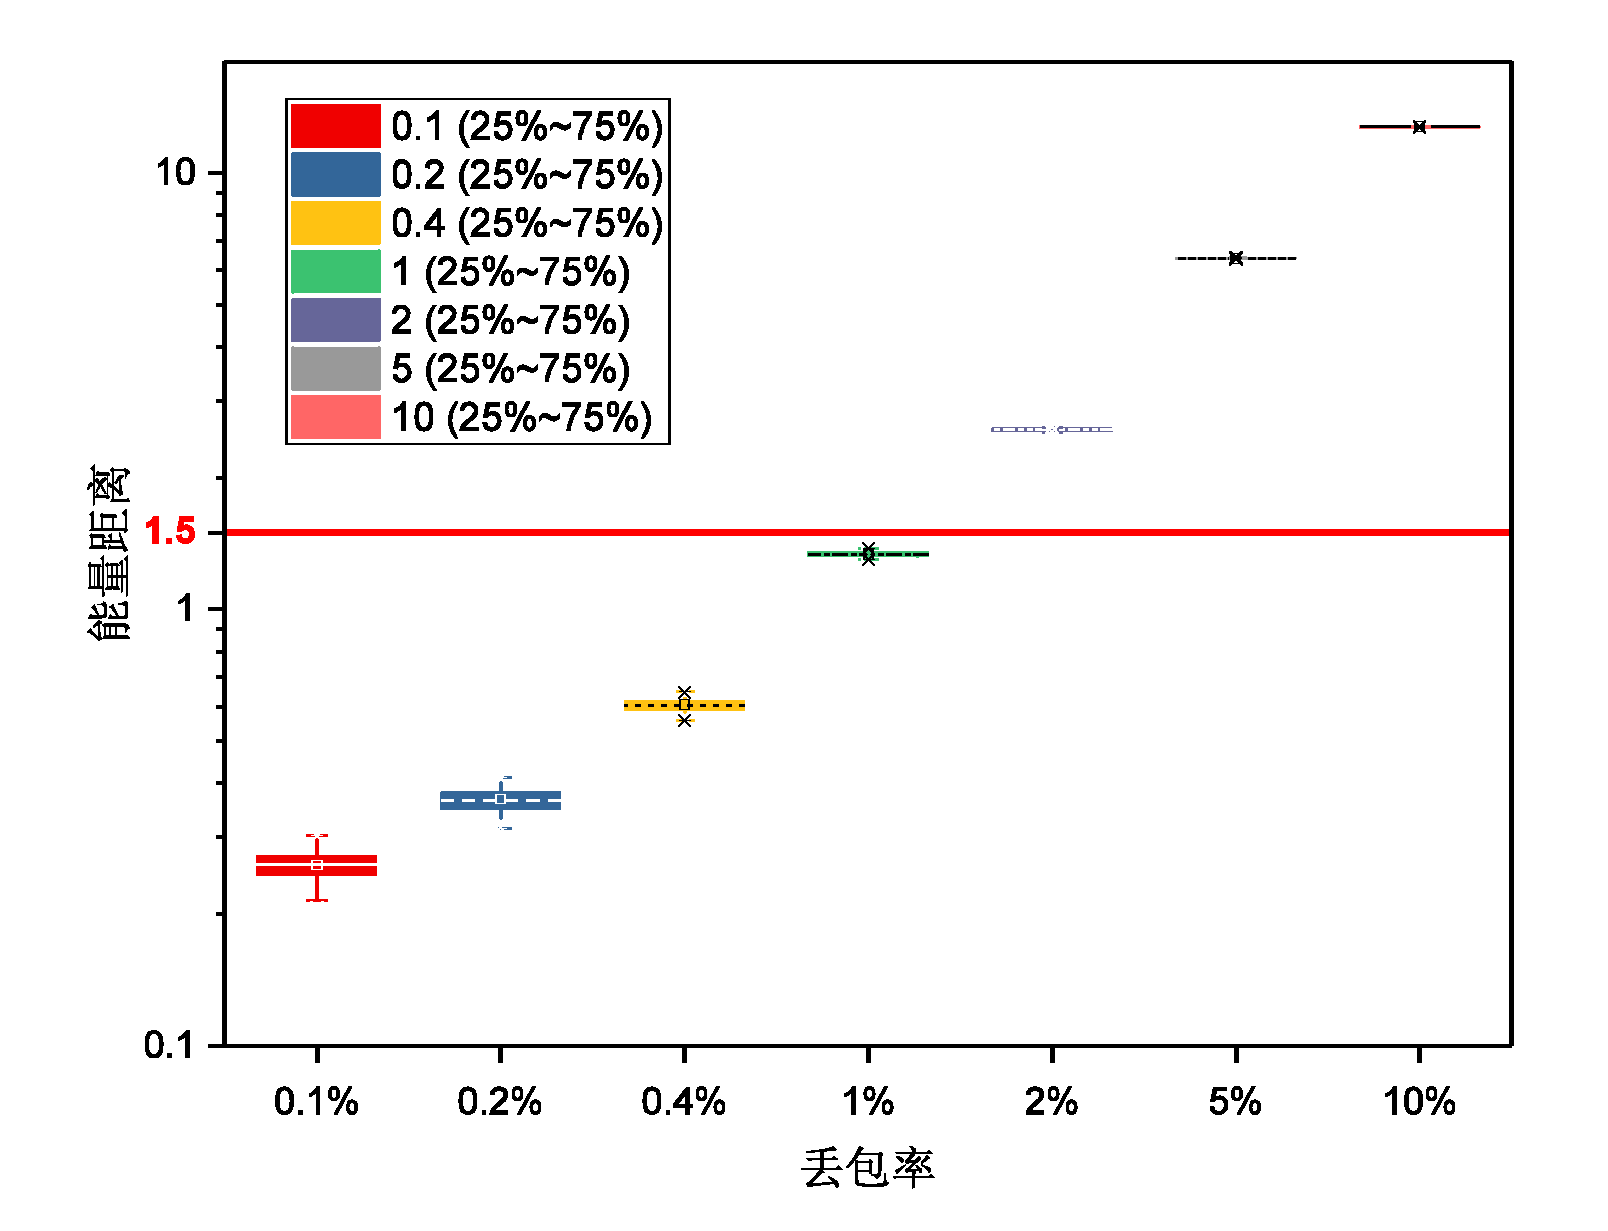
\includegraphics[width=0.48\textwidth]{chapters/chapter3/figures/win100-ed-good.pdf}
        }
        \subfigure[区间长度为200时Excellent场景能量距离的箱线图]{
            \label{fig:3:result:win200:ed:excellent}
            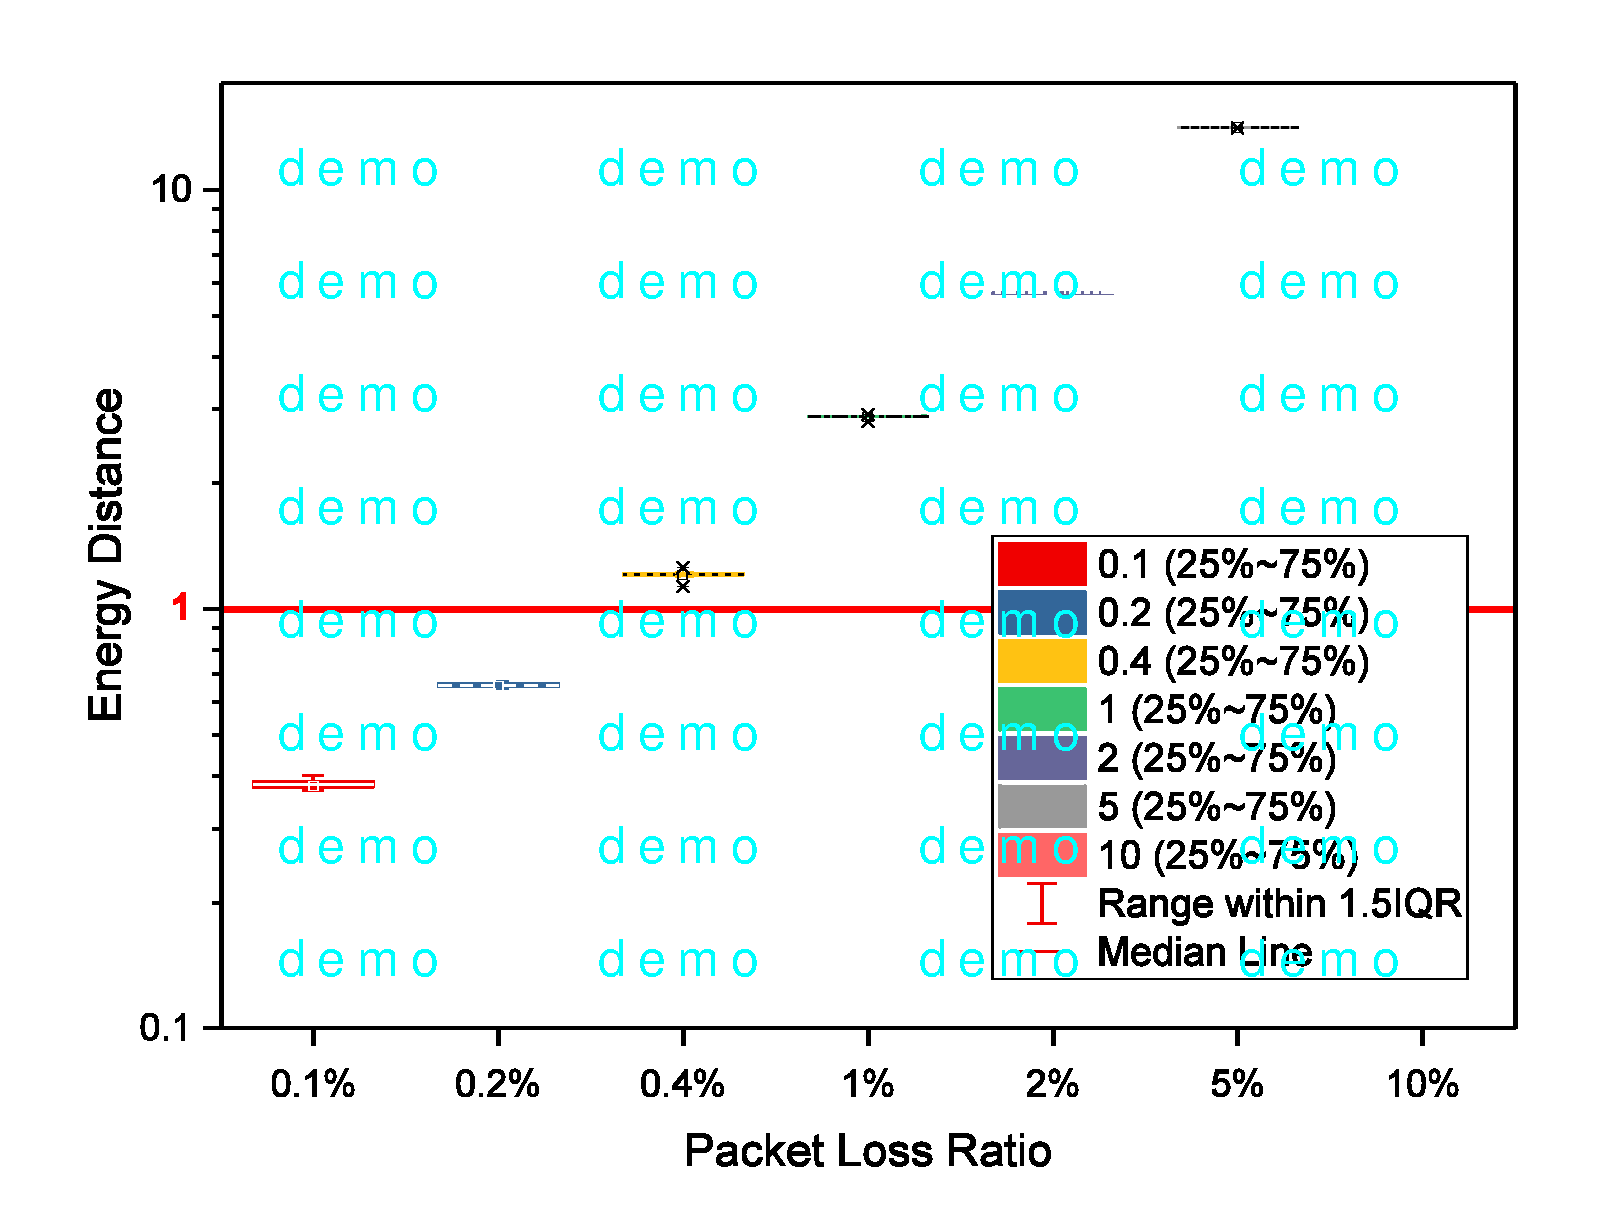
\includegraphics[width=0.48\textwidth]{chapters/chapter3/figures/win200-ed-excellent.pdf}
        }
        \subfigure[区间长度为200时Good场景能量距离的箱线图]{
            \label{fig:3:result:win200:ed:good}
            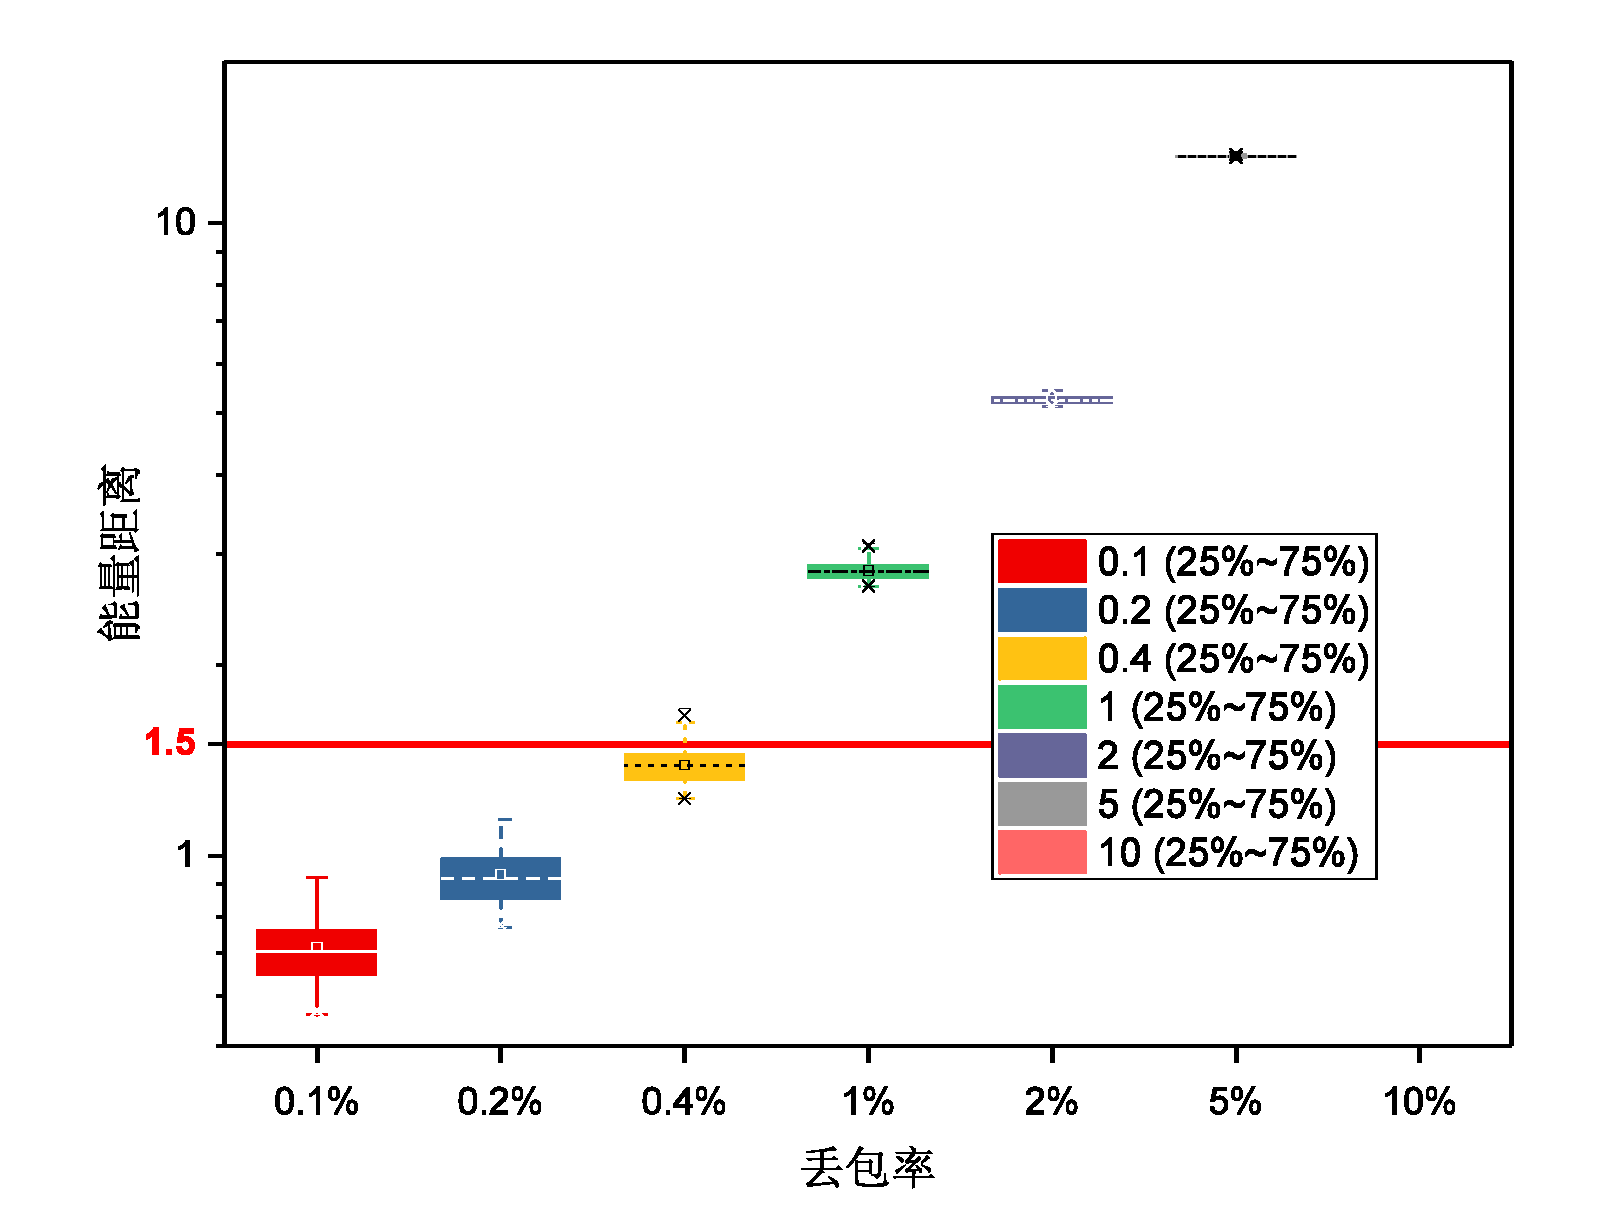
\includegraphics[width=0.48\textwidth]{chapters/chapter3/figures/win200-ed-good.pdf}
        }
        \caption{区间丢包数能量距离检测的箱线图}
        \label{fig:3:result:win:ed}
	\end{figure}
}

如图\ \nref{fig:3:result:win:wd},区间长度为100时,只有主动丢包率$\le 1\ \%$才通过Wasserstein距离检测;而区间长度扩展到200时,只有主动丢包率$\le 0.4\ \%$才通过检测。如图\ \nref{fig:3:result:win:ed},能量距离检测结果类似Wasserstein距离检测结果,当区间长度为100时,主动丢包率$\le 1\ \%$才通过检测;而区间长度为200时,主动丢包率$\le 0.4\ \%$才有较高的几率通过检测。

\subsection{总结}
通过分析检测结果,相对距离有效反映了CDF曲线的差异,结合K-L散度得到更全面的检测结果。实验结果证明,结合区间丢包数分布和连续丢包数分布后,有效补充了基于IPD的检测方法。根据表\ \nref{tab:3:detect-sum}中设定的10条量化评估子项,汇总得到最终的检出率表。

\insertTable{
	\begin{table}[htbp]
    \centering
    \caption{Excellent场景下时间隐通道检出率汇总表}
    \label{tab:3:result-sum:excellent}
        \begin{threeparttable}
            \begin{tabular*}{0.99\textwidth}{@{\extracolsep{\fill}}ccccccccc}
                \toprule
                \multirow{2.5}{*}{检测对象} & \multirow{2.5}{*}{检测方法} & \multicolumn{7}{c}{主动丢包率} \\
                \cmidrule(l){3-9}
                & & 10\% & 5\% & 2\% & 1\% & 0.4\% & 0.2\% & 0.1\% \\
                \midrule
                \multirow{5}{*}{IPD分布} & K-S检验 & 100\% & 100\% & 100\% & 0\% & 0\% & 0\% & 0\% \\
                & t检验,rank检验\tnote{1} & 100\% & 100\% & 100\% & 100\% & 0\% & 0\% & 0\% \\
                & K-L散度 & 0\% & 0\% & 0\% & 0\% & 0\% & 0\% & 0\% \\
                & Wasserstein距离 & 0\% & 0\% & 0\% & 0\% & 0\% & 0\% & 0\% \\
                & 能量距离 & 100\% & 0\% & 0\% & 0\% & 0\% & 0\% & 0\% \\
                \\
                \multirow{3}{*}{连续丢包数} & K-L散度 & 100\% & 100\% & 100\% & 100\% & 100\% & 0\% & 0\% \\
                & Wasserstein距离 & 0\% & 0\% & 0\% & 0\% & 0\% & 0\% & 0\% \\
                & 能量距离 & 100\% & 100\% & 0\% & 0\% & 0\% & 0\% & 0\% \\
                \\
                \multirow{2}{*}{区间丢包数} & Wasserstein距离 & 100\% & 100\% & 100\% & 100\% & 0\% & 0\% & 0\% \\
                & 能量距离 & 100\% & 100\% & 100\% & 100\% & 0\% & 0\% & 0\% \\
                \bottomrule
            \end{tabular*}
            \begin{tablenotes}
                \footnotesize
                \item[1] Welch's t检验与Mann–Whitney rank检验通过一种即可
            \end{tablenotes}
        \end{threeparttable}
    \end{table}
}

\insertTable{
	\begin{table}[htbp]
    \centering
    \caption{Good场景下时间隐通道检出率汇总表}
    \label{tab:3:result-sum:good}
        \begin{threeparttable}
            \begin{tabular*}{0.99\textwidth}{@{\extracolsep{\fill}}ccccccccc}
                \toprule
                \multirow{2.5}{*}{检测对象} & \multirow{2.5}{*}{检测方法} & \multicolumn{7}{c}{主动丢包率} \\
                \cmidrule(l){3-9}
                & & 10\% & 5\% & 2\% & 1\% & 0.4\% & 0.2\% & 0.1\% \\
                \midrule
                \multirow{5}{*}{IPD分布} & K-S检验 & 100\% & 100\% & 100\% & 0\% & 0\% & 0\% & 0\% \\
                & t检验,rank检验\tnote{1} & 100\% & 100\% & 0\% & 0\% & 0\% & 0\% & 0\% \\
                & K-L散度 & 0\% & 0\% & 0\% & 0\% & 0\% & 0\% & 0\% \\
                & Wasserstein距离 & 0\% & 0\% & 0\% & 0\% & 0\% & 0\% & 0\% \\
                & 能量距离 & 100\% & 0\% & 0\% & 0\% & 0\% & 0\% & 0\% \\
                \\
                \multirow{3}{*}{连续丢包数} & K-L散度 & 100\% & 100\% & 100\% & 0\% & 0\% & 0\% & 0\% \\
                & Wasserstein距离 & 100\% & 100\% & 0\% & 0\% & 0\% & 0\% & 0\% \\
                & 能量距离 & 100\% & 100\% & 100\% & 0\% & 0\% & 0\% & 0\% \\
                \\
                \multirow{2}{*}{区间丢包数} & Wasserstein距离 & 100\% & 100\% & 100\% & 100\% & 11\% & 0\% & 0\% \\
                & 能量距离 & 100\% & 100\% & 100\% & 100\% & 11\% & 0\% & 0\% \\
                \bottomrule
            \end{tabular*}
            \begin{tablenotes}
                \footnotesize
                \item[1] Welch's t检验与Mann–Whitney rank检验通过一种即可
            \end{tablenotes}
        \end{threeparttable}
    \end{table}
}

如表\ \nref{tab:3:result-sum:excellent}及表\ \nref{tab:3:result-sum:good},不同方法的检出率存在差异,不同场景的检出率也存在差距。Excellent场景中,连续丢包数及区间丢包数的检测,能够准确体现主动丢包的影响。当主动丢包的比例降低,超过了检测方法的灵敏度,时间隐通道将无法被检测出来。Good场景中,由于信道中已经存在一定比例的丢包事件,连续丢包数的检测能力减弱;但基于区间丢包数的检测方法,能够进一步区分随机丢包,因此具有较好的检测效果。

\insertTable{
	\begin{table}[htbp]
      \centering
      \caption{时间隐通道检出率汇总表}
      \label{tab:3:result-sum:all}
          \begin{tabular*}{0.99\textwidth}{@{\extracolsep{\fill}}cccccccc}
            \toprule
            \multirow{2.5}{*}{场景} 
            & \multicolumn{7}{c}{主动丢包率} \\
            \cmidrule(l){2-8}
            & 10\ \% & 5\ \% & 2\ \% & 1\ \% & 0.4\ \% & 0.2\ \% & 0.1\ \% \\ 
            \midrule
            Excellent & 100\ \% & 100\ \% & 100\ \% & 100\ \% & 100\ \% & 0\ \% & 0\ \% \\
            Good & 100\ \% & 100\ \% & 100\ \% & 100\ \% & 11\ \% & 0\ \% & 0\ \% \\
            \bottomrule
          \end{tabular*}
    \end{table}
}

汇总所有检测子项的结果,时间隐通道检测能力如表\ \nref{tab:3:result-sum:all}。由表可知,该检测方法对主动丢包敏感,只有时间隐通道的主动丢包率控制在$0.4\ \%$以下,才有可能通过检测。